\documentclass{patmorin}
\listfiles
\usepackage[utf8]{inputenc}
\usepackage{amsthm,amsmath,graphicx}
\usepackage{pat}
\usepackage[letterpaper]{hyperref}
\usepackage[dvipsnames]{color}
\definecolor{linkblue}{named}{Blue}
\hypersetup{colorlinks=true, linkcolor=linkblue,  anchorcolor=linkblue,
citecolor=linkblue, filecolor=linkblue, menucolor=linkblue,
urlcolor=linkblue, pdfcreator=Me, pdfproducer=Me} \setlength{\parskip}{1ex}


\DeclareMathOperator{\sign}{sign}
\DeclareMathOperator{\xmax}{xmax}
\DeclareMathOperator{\xmin}{xmin}
\DeclareMathOperator{\ymax}{ymax}
\DeclareMathOperator{\ymin}{ymin}
\DeclareMathOperator{\survivors}{survivors}

\usepackage{array}


% To reduce space in lists
\usepackage{enumitem}  
\setlist{noitemsep}

%\usepackage[skip=0pt]{caption}

\title{\MakeUppercase{More Turán-Type Theorems for Triangles in Convex Point Sets}\thanks{This research is partially funded by NSERC.}}
\author{Authors TBD}


\newcommand{\edgea}{\raisebox{-.1ex}{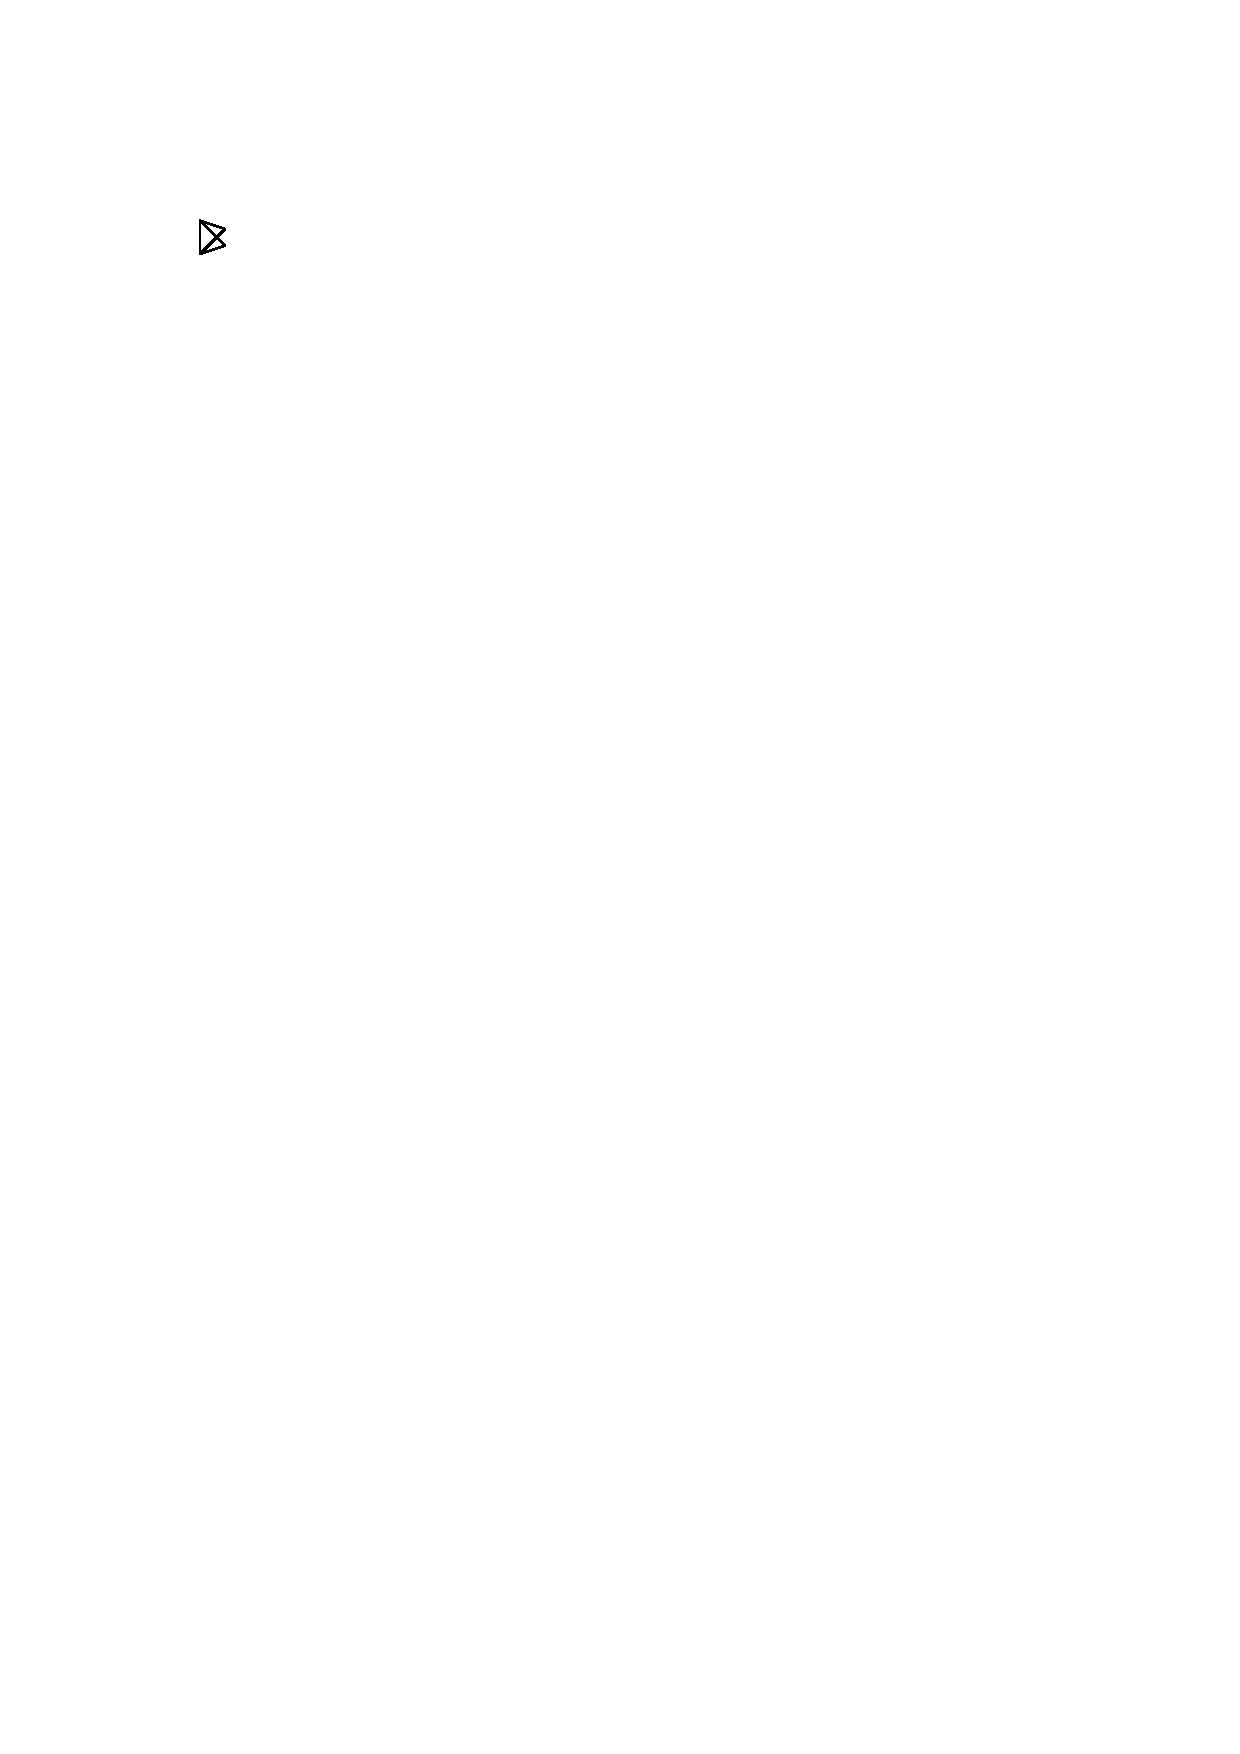
\includegraphics[height=1.6ex]{figs/triangles-edge-1}}}
\newcommand{\edgeb}{\raisebox{-.1ex}{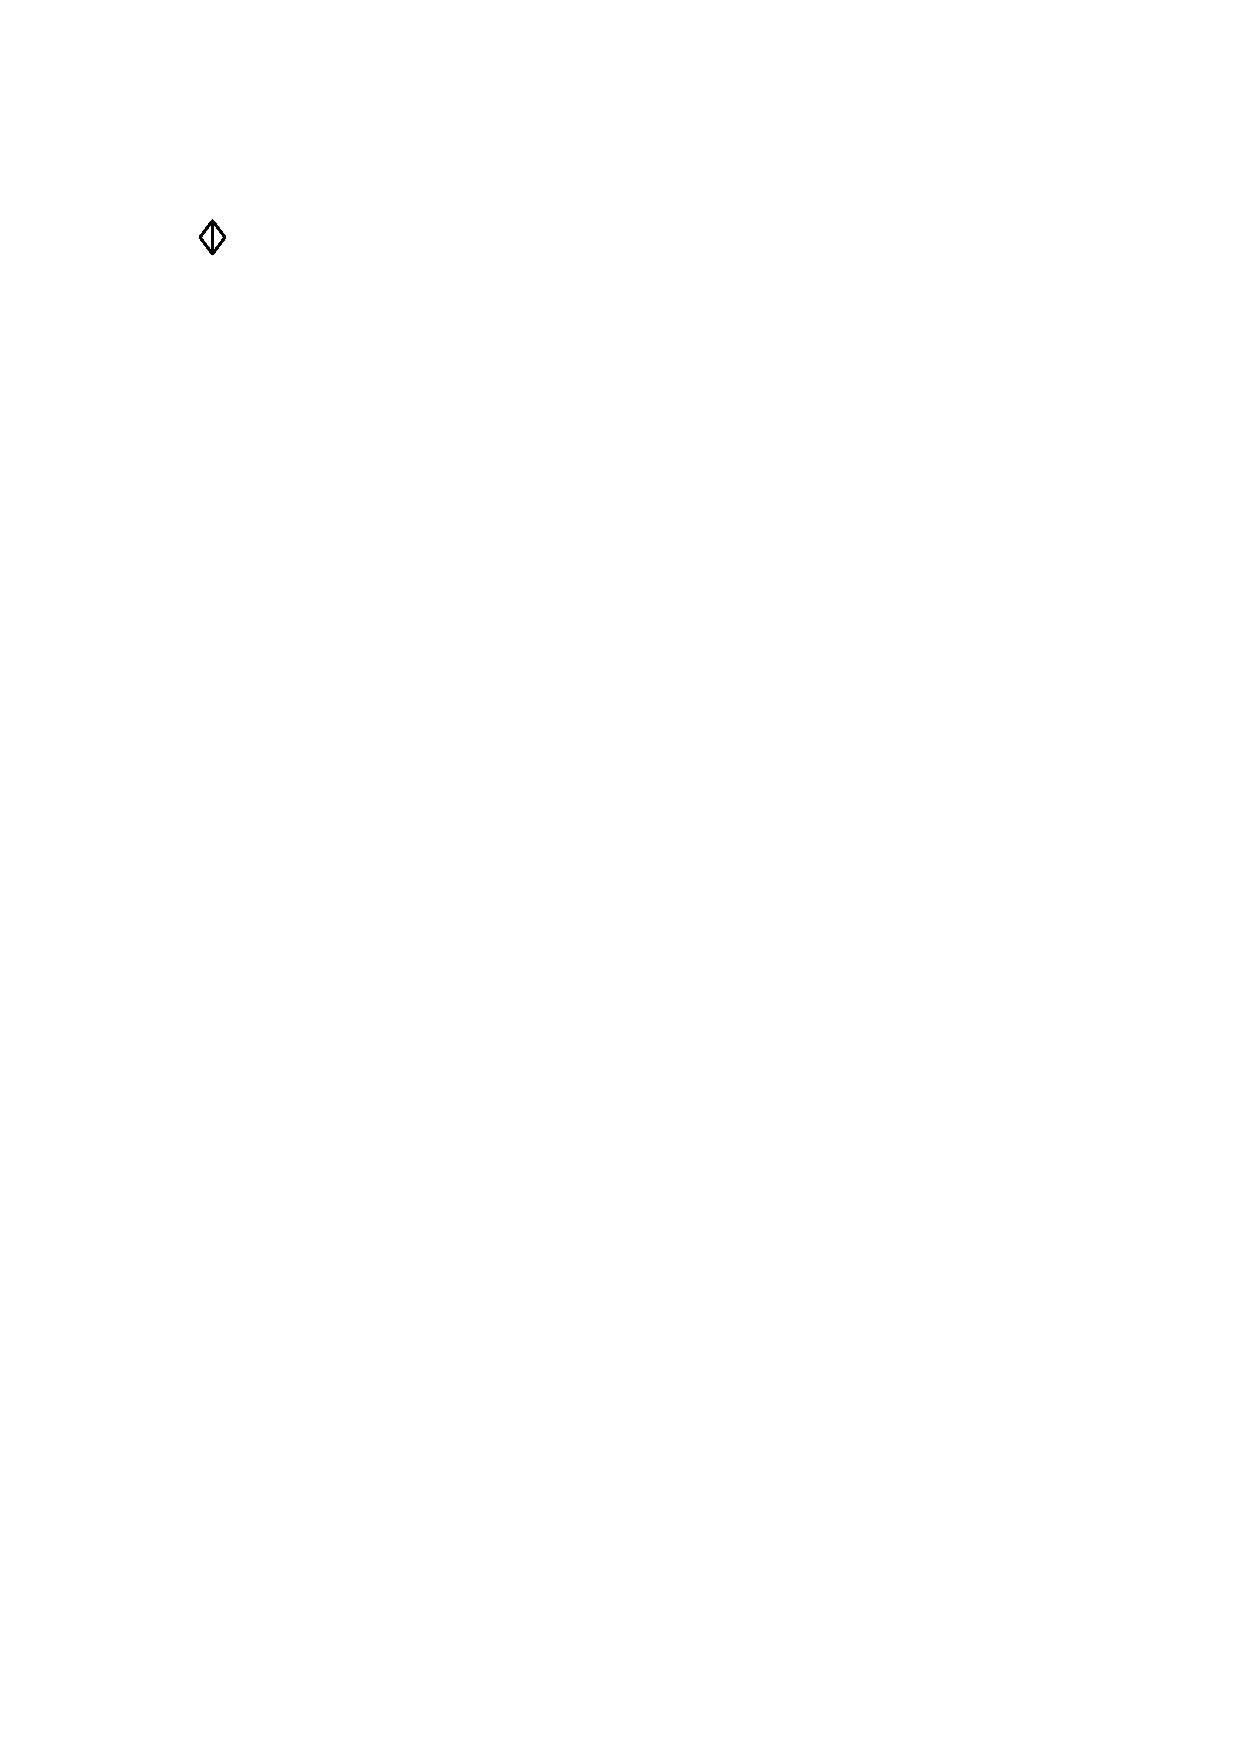
\includegraphics[height=1.6ex]{figs/triangles-edge-2}}}


\newcommand{\vertexa}{\raisebox{-.1ex}{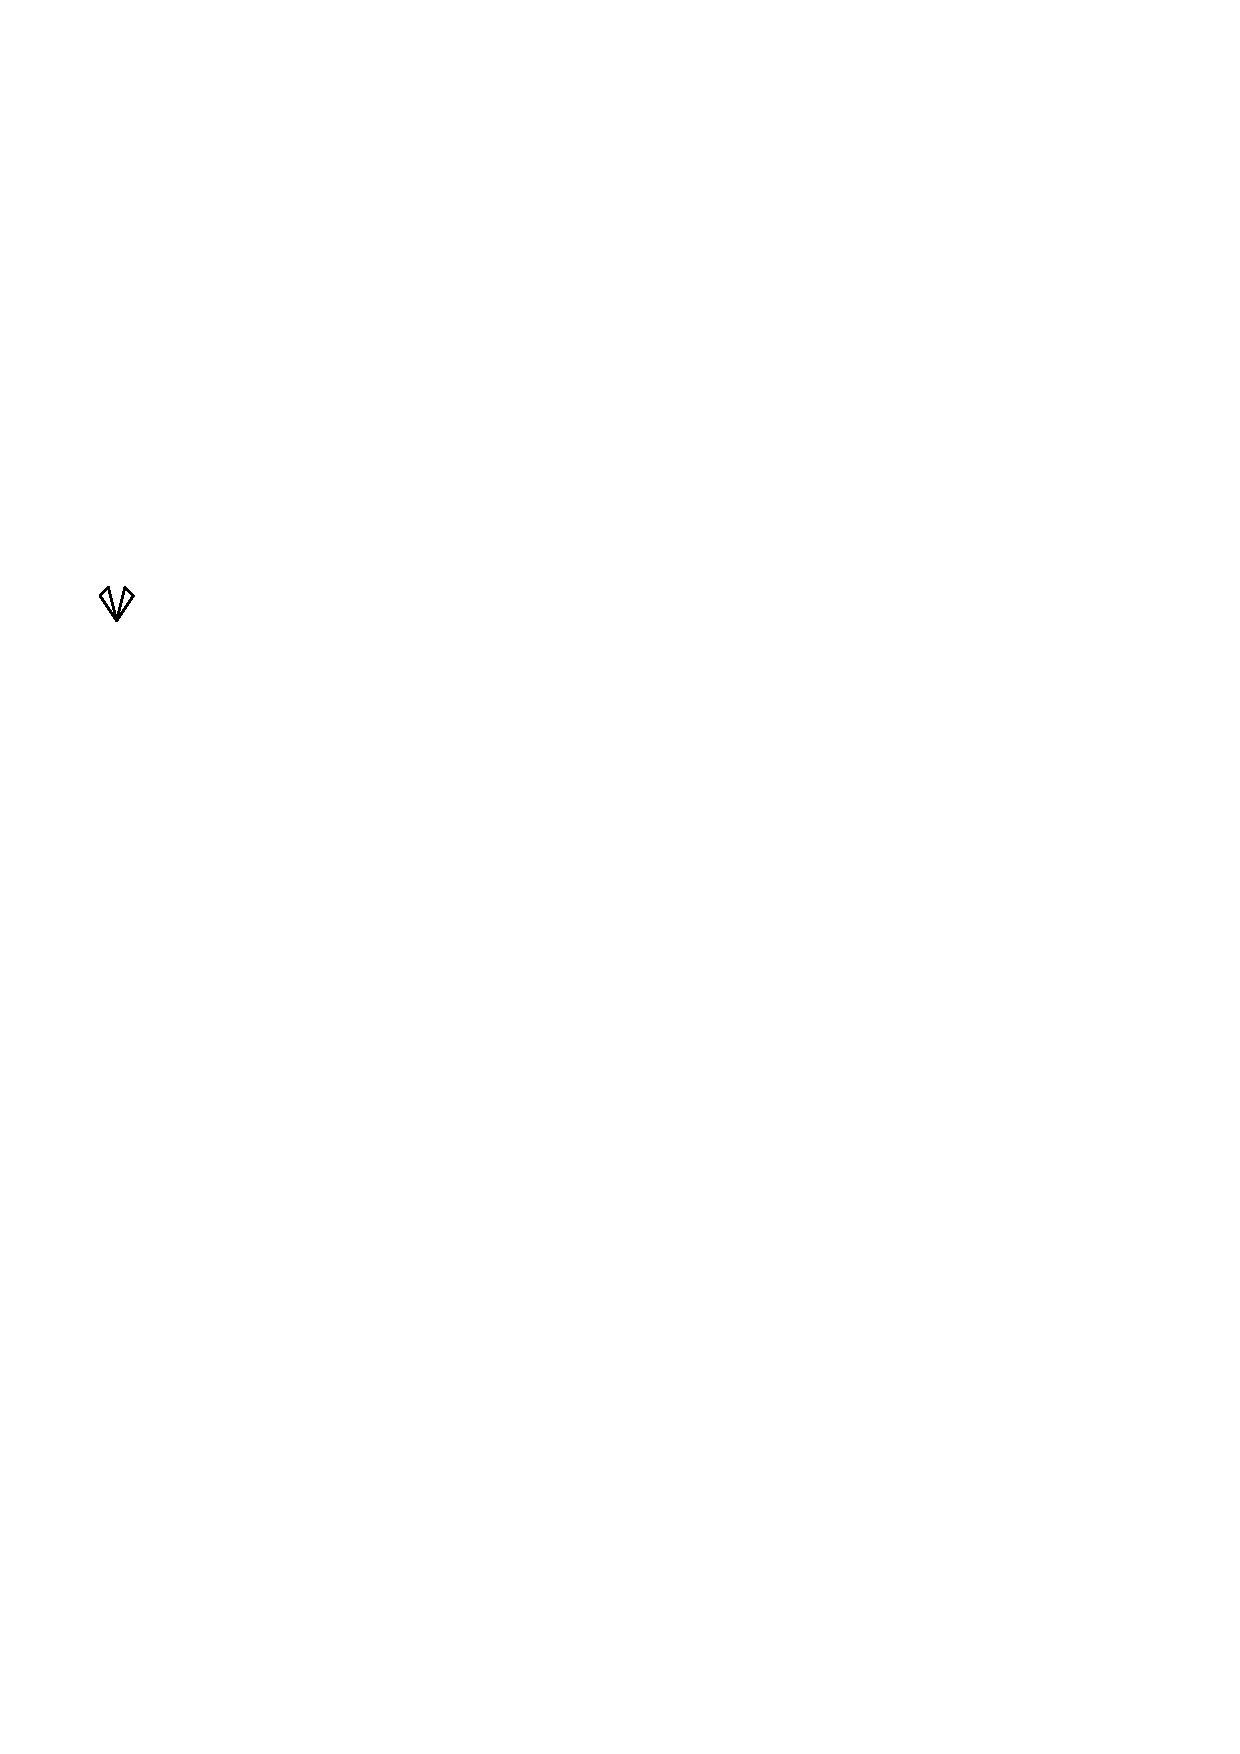
\includegraphics[height=1.6ex]{figs/triangles-vertex-1}}}
\newcommand{\vertexb}{\raisebox{-.1ex}{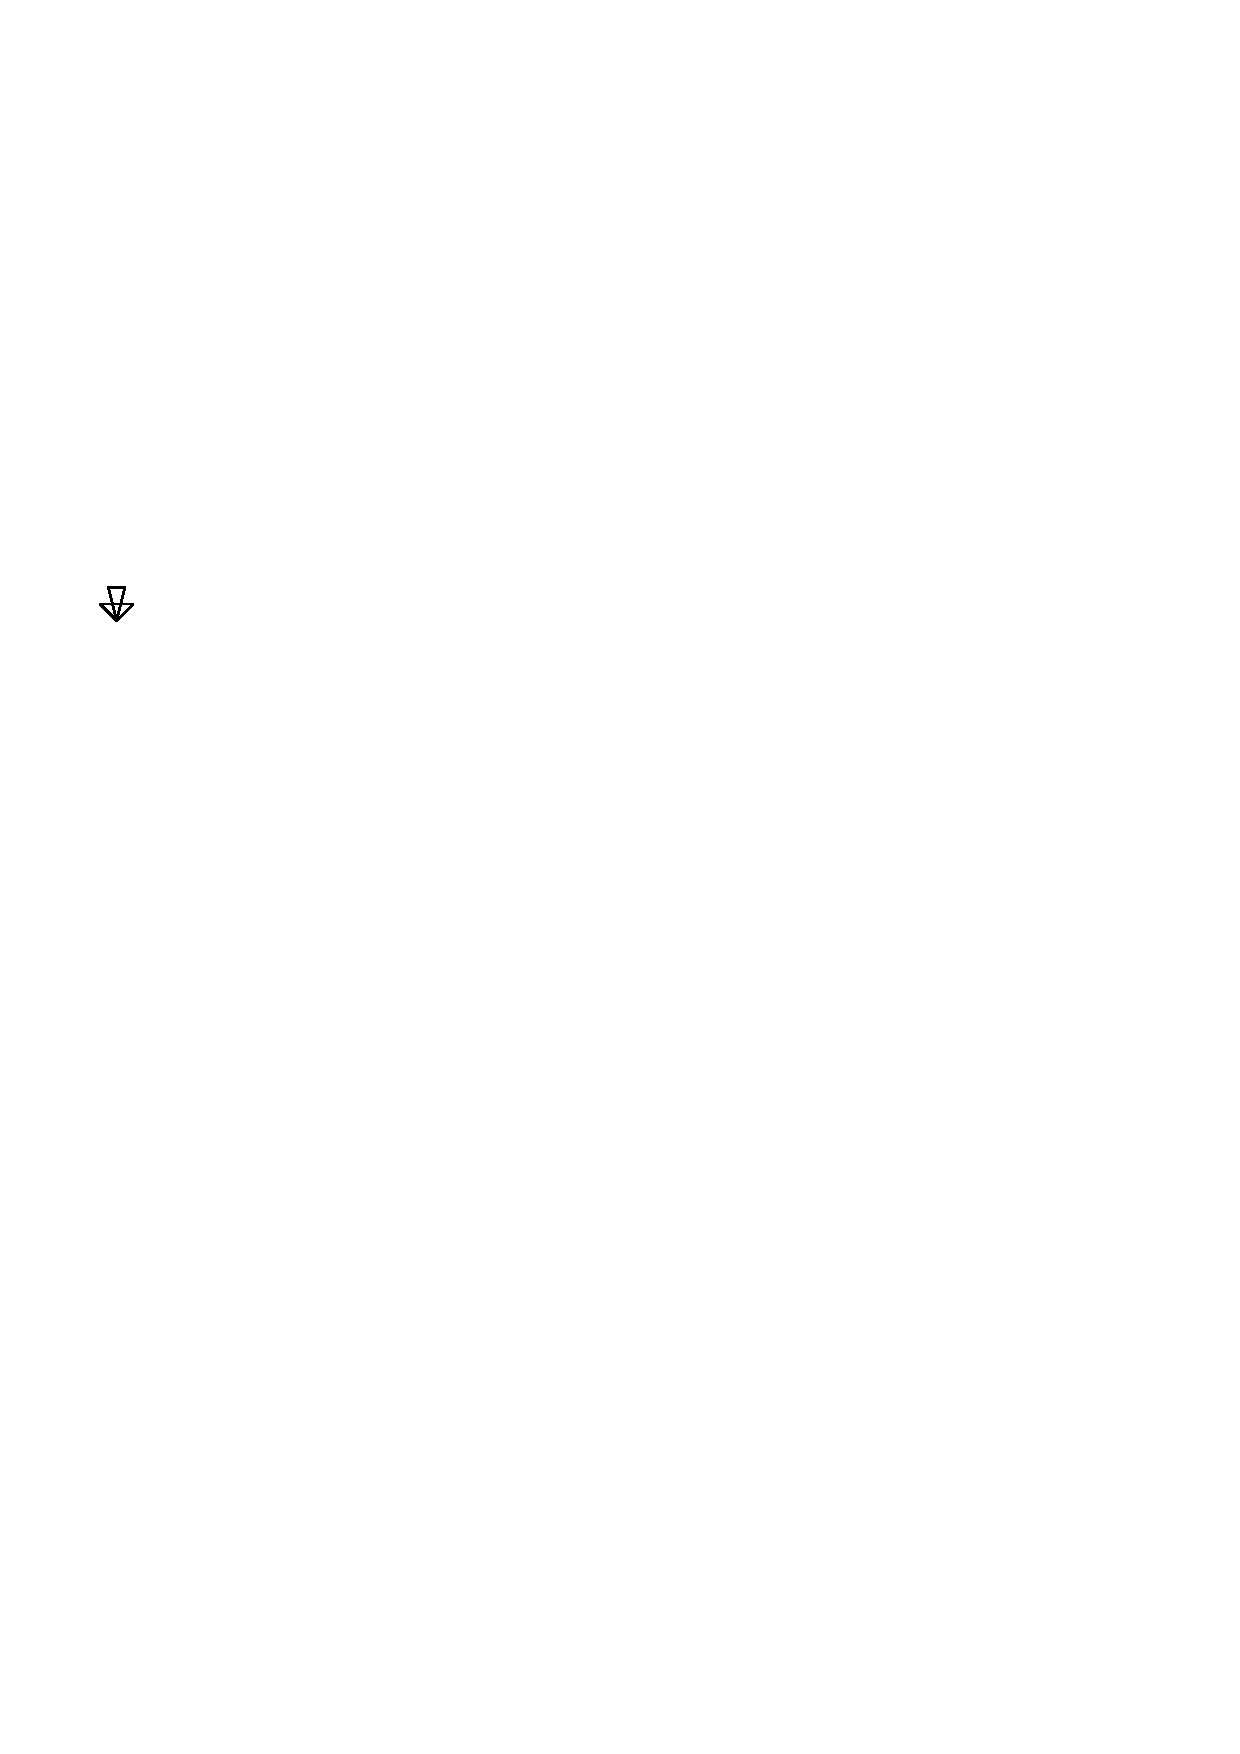
\includegraphics[height=1.6ex]{figs/triangles-vertex-2}}}
\newcommand{\vertexc}{\raisebox{-.1ex}{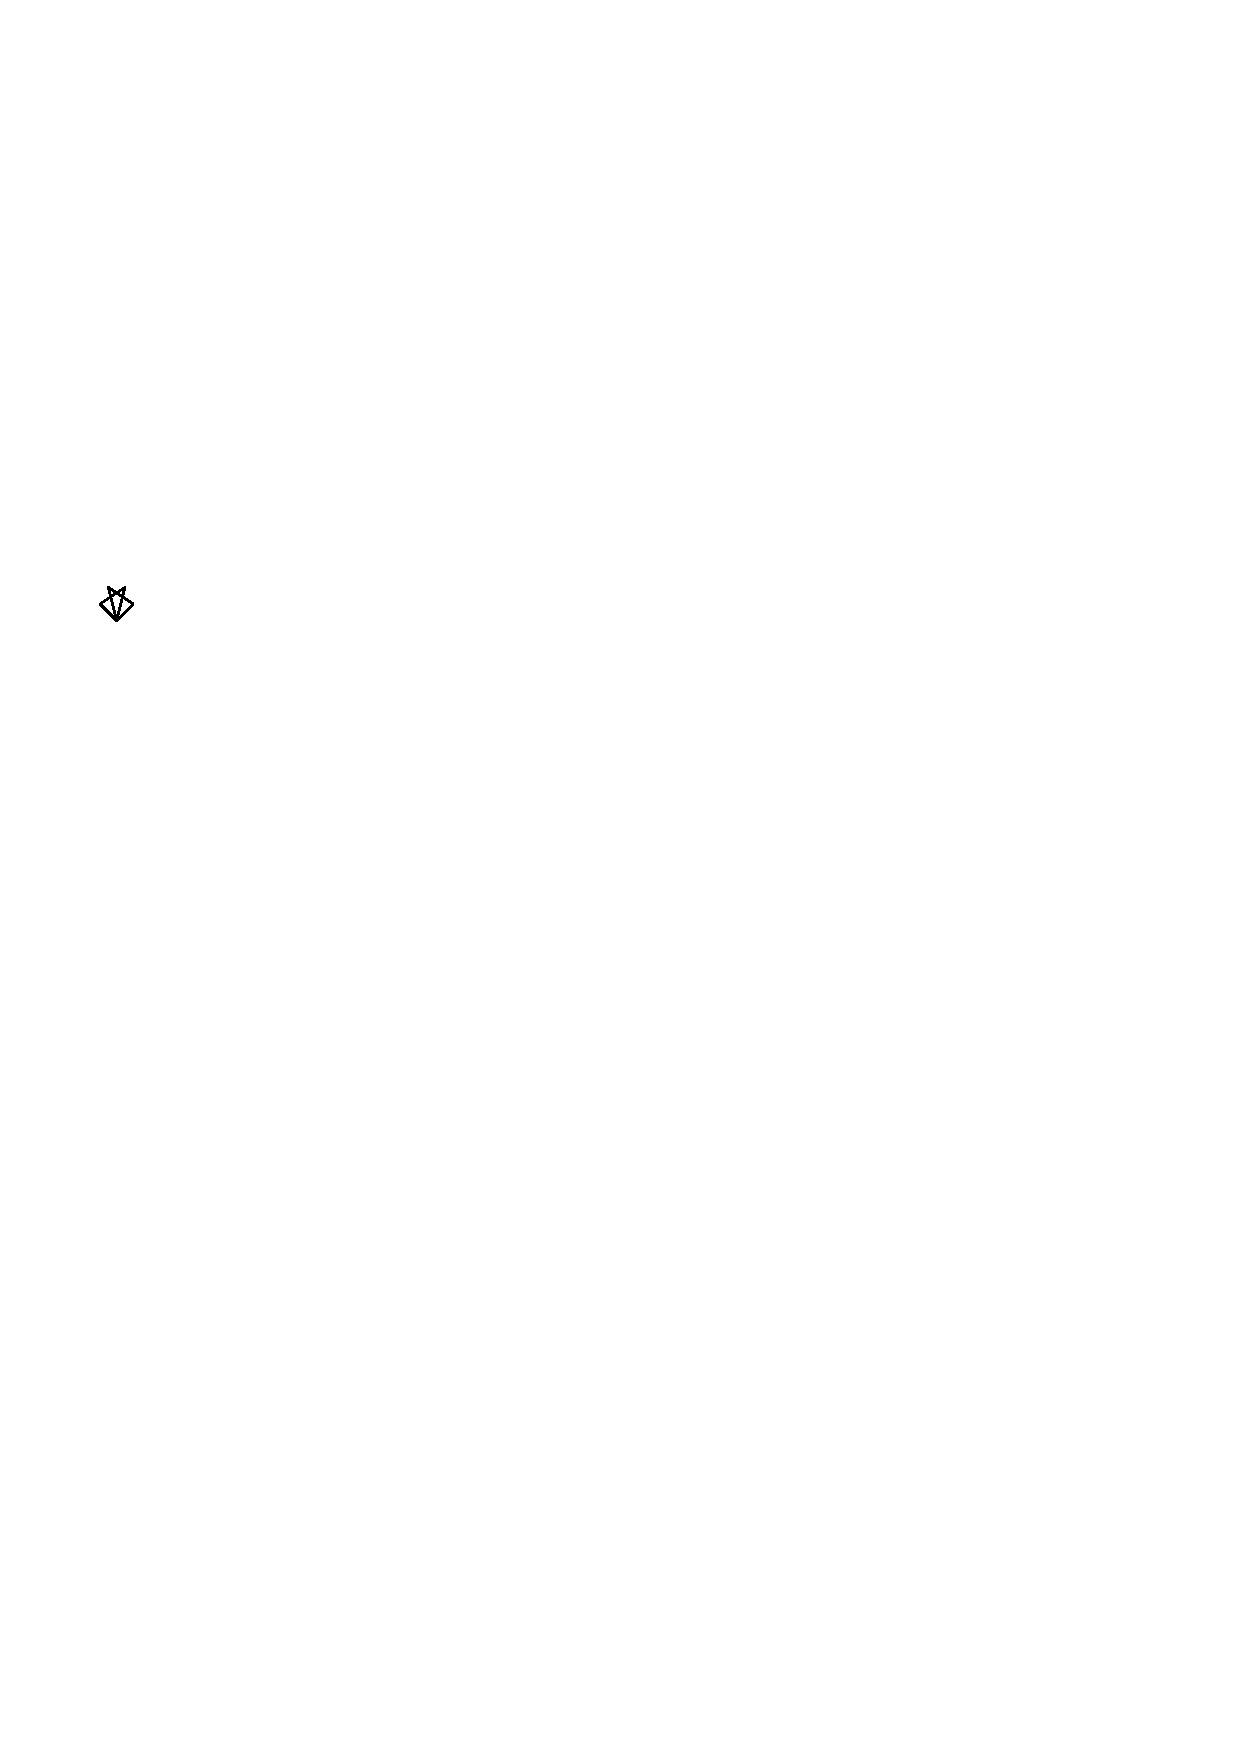
\includegraphics[height=1.6ex]{figs/triangles-vertex-3}}}

\newcommand{\disjointa}{\raisebox{-.1ex}{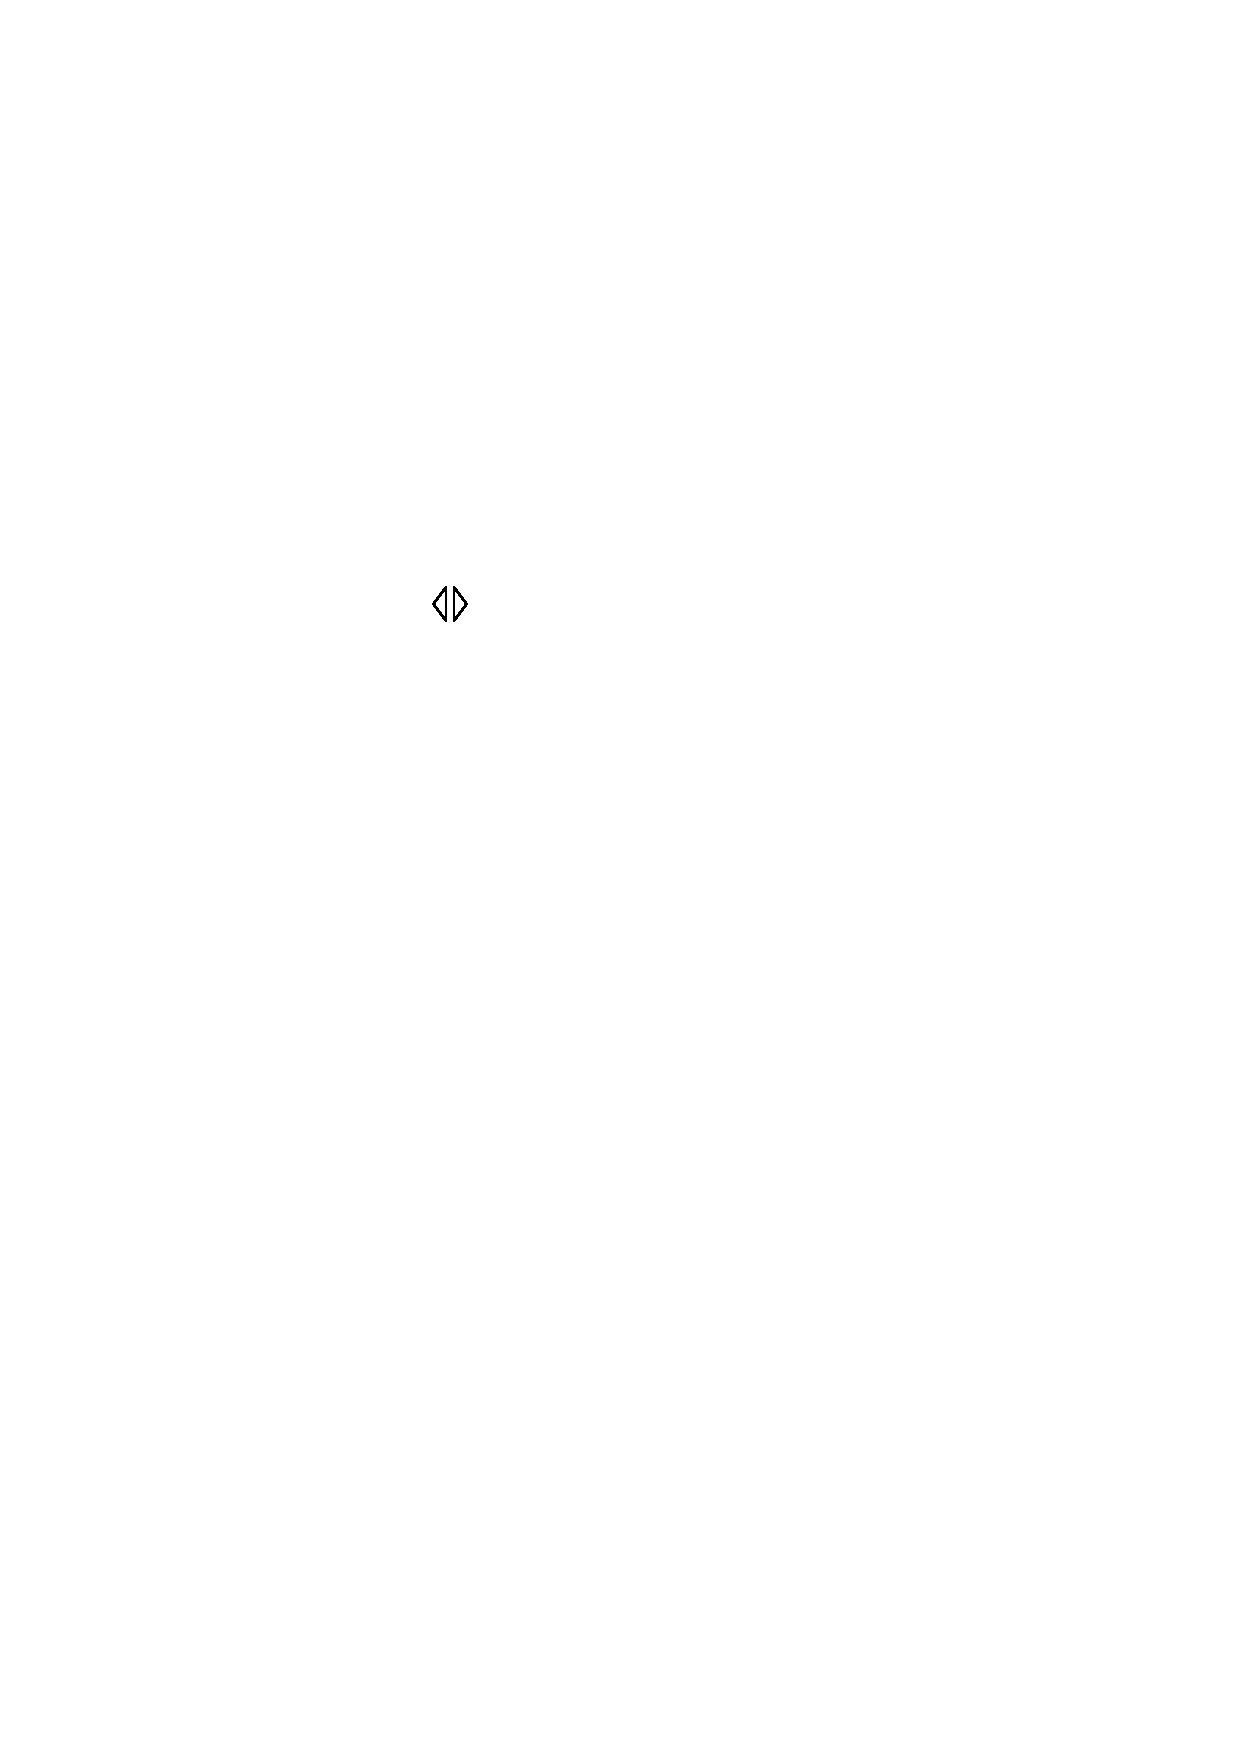
\includegraphics[height=1.6ex]{figs/triangles-disjoint-1}}}
\newcommand{\disjointb}{\raisebox{-.1ex}{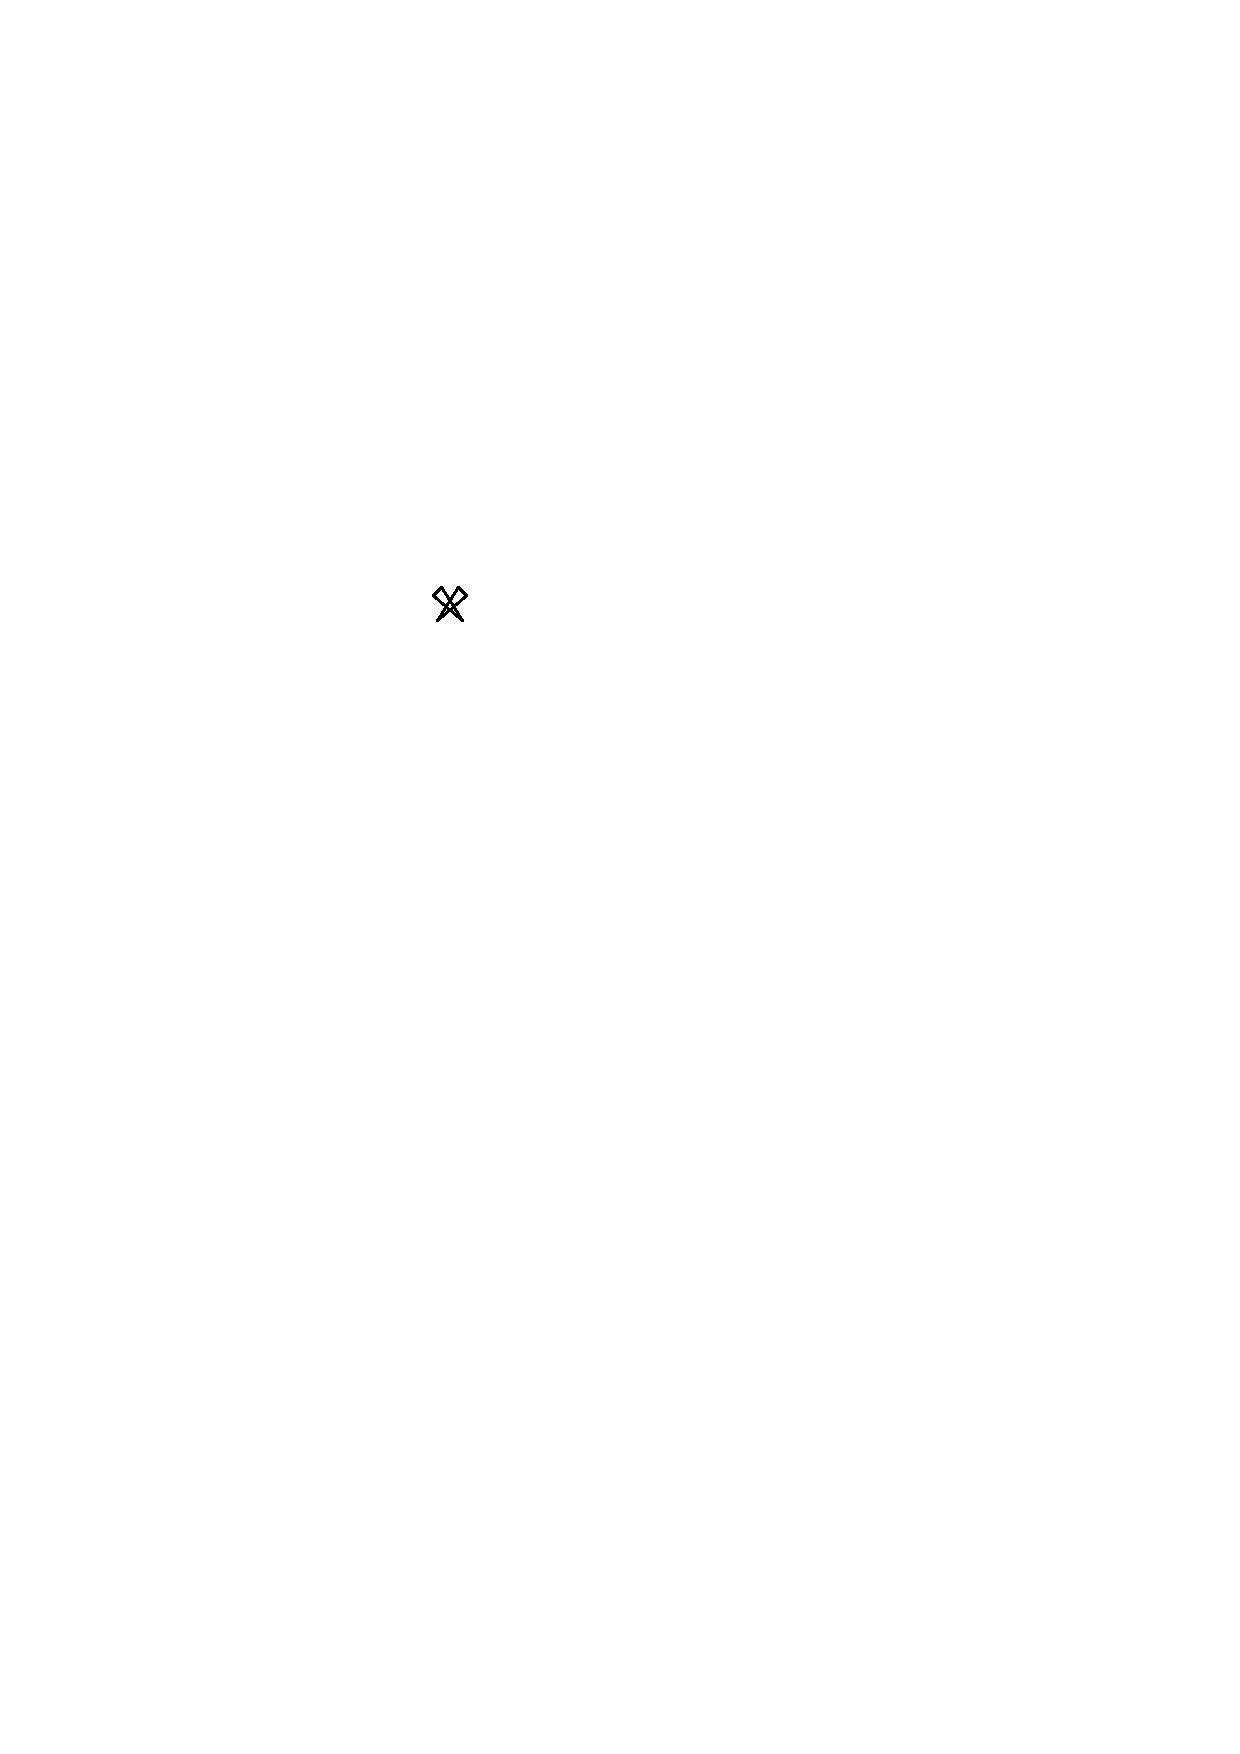
\includegraphics[height=1.6ex]{figs/triangles-disjoint-2}}}
\newcommand{\disjointc}{\raisebox{-.1ex}{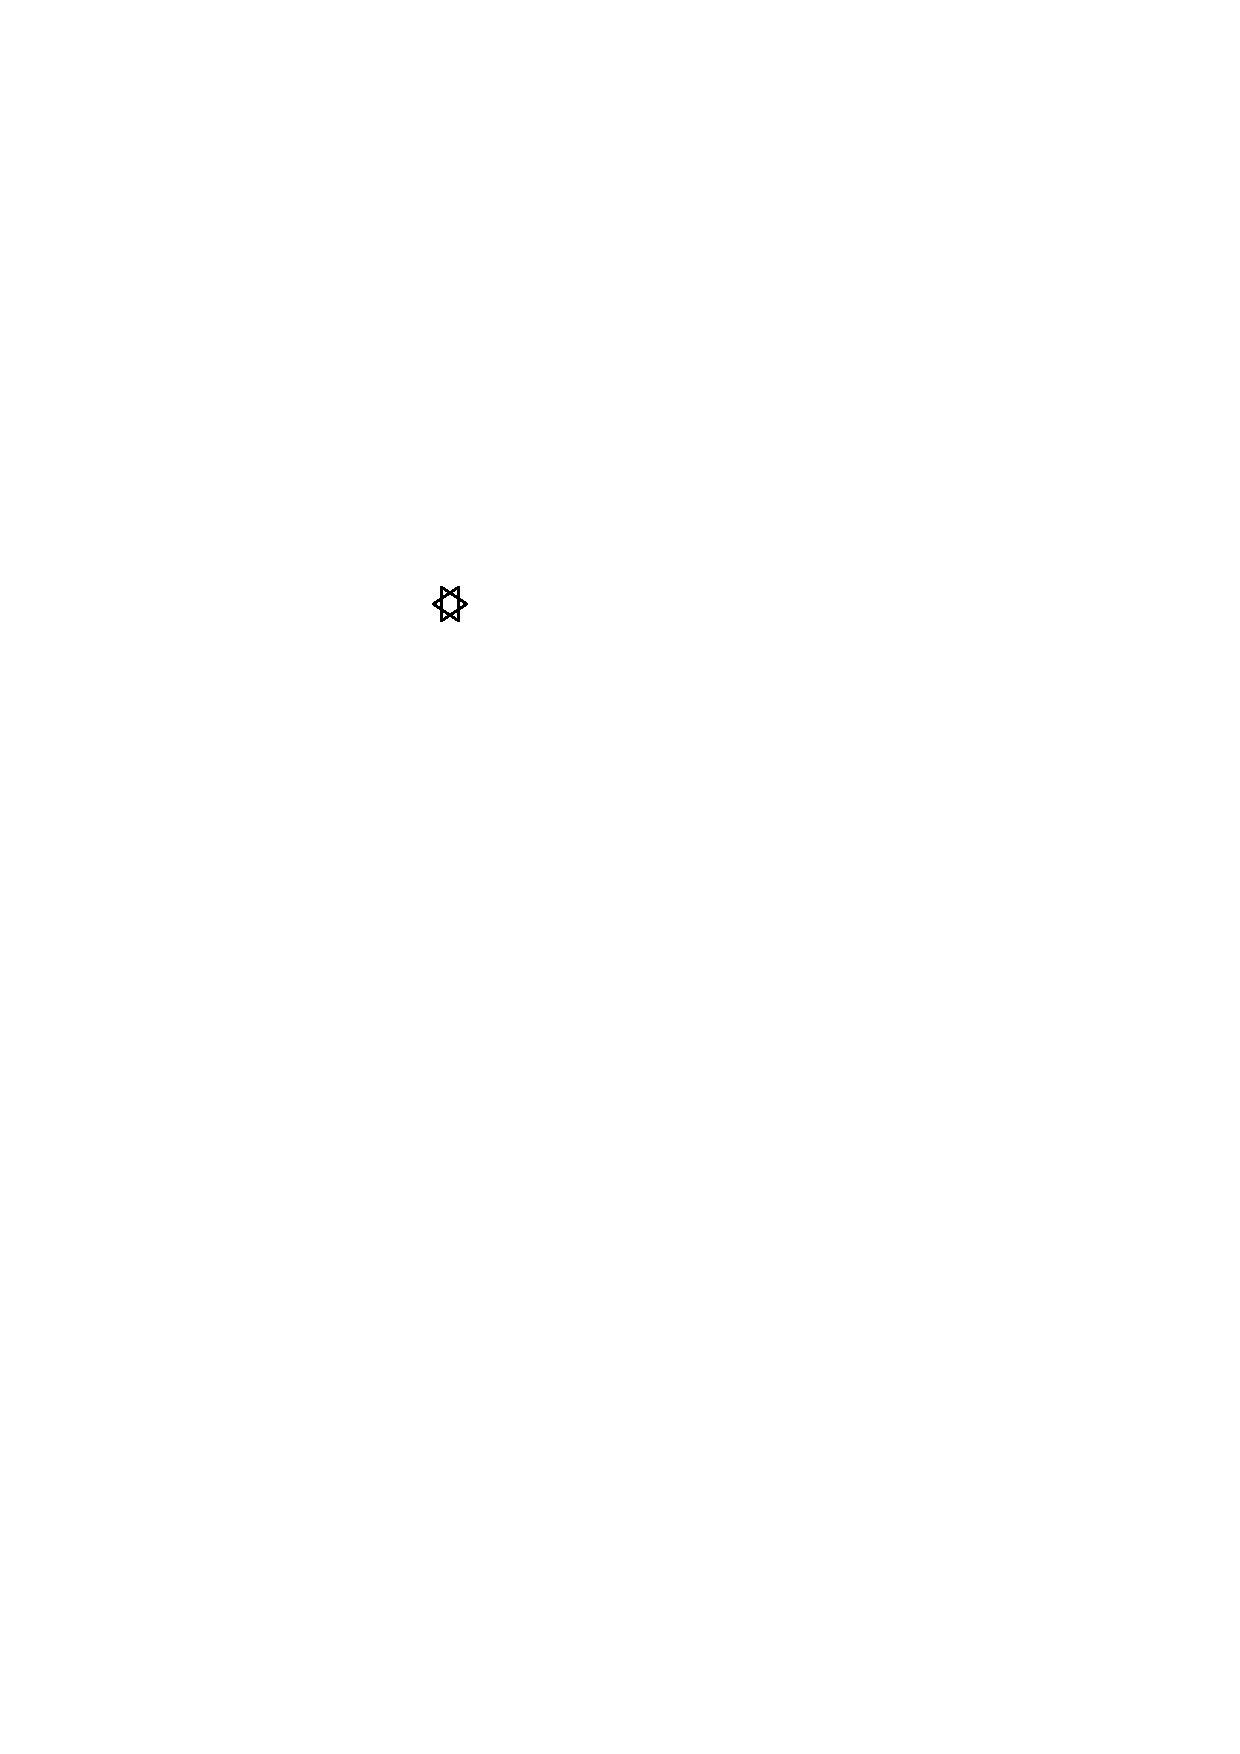
\includegraphics[height=1.6ex]{figs/triangles-disjoint-3}}}

\DeclareMathOperator{\ex}{ex}
\DeclareMathOperator{\on}{\overline{ex}}



%\usepackage{lineno}
%\linenumbers

\begin{document}
\maketitle

\begin{abstract}
  We study the following family of problems: Given a set of $n$ points
  in convex position, what is the maximum number triangles one can create
  having these points as vertices while avoiding certain \emph{forbidden
  configurations}.  As forbidden configurations we consider all 8 ways
  in which a pair of triangles in such a point set can interact.
\end{abstract}



\section{Introduction}

Let $t_1$ and $t_2$ be a pair of distinct triangles whose (4--6) vertices
are in convex position.  There are 8 combinatorially distinct ways that
these triangle can interact:  2 ways in which the triangles can share
an edge (\edgea\ and \edgeb), 3 ways in which the triangles can share a
single vertex (\vertexa, \vertexb, and \vertexc), and 3 ways in which
the triangles can have no vertices in common (\disjointa, \disjointb,
and \disjointc).

We consider the following class of problems:  Given a set, $X$,
of combinatorial configurations of pairs of triangles, what is the
largest set, $S$, of triangles one can create whose vertices are $n$
points in convex position, and such that no pair of triangles in $S$
forms a configuration in $X$.  We call the size of this set $\ex(n,X)$.
For example, 
\begin{equation}
    \ex(n,\{\edgea,\vertexb,\vertexc,\disjointb,\disjointc\}) = n-2 \enspace .
\end{equation}
This is because the set
$X=\{\edgea,\vertexb,\vertexc,\disjointb,\disjointc\}$ in this case
forbids any form of crossings between the edges of triangles. Thus,
the number maximum number of triangles we can have while avoiding $X$
is the number of triangles in a triangulation of a convex $n$-gon,
i.e., $n-2$. One of the results in this paper is that nearly the
same bound holds even if we allow the $\disjointb$ and $\disjointc$
configuration. In particular, our \thmref{blech} shows that
$\ex(n,\{\edgea,\vertexb,\vertexc\}) \in O(n\log n)$.

Sometimes it is more natural to describe the allowable configurations than the forbidden configurations. For this, we use the notation 
\[
   \on(n,X) = \ex(n,\{\edgea,\edgeb,\vertexa,\vertexb,\vertexc,
                       \disjointa,\disjointb,\disjointc\} \setminus X) \enspace .
\]



\begin{table}
\begin{center}
\begin{tabular}{m{.55\textwidth}m{.4\textwidth}}
  \hline
  $\ex(n,\{\edgeb\})\in \Theta(n^3)$ & \cite{brass:turan} \\
  $\ex(n,\{\edgea\})\in \Theta(n^2)$ & \cite{brass:turan} \\
  \hline
  $\ex(n,\{\vertexa\})\in \Theta(n^3)$ & \cite{brass:turan} \\
  $\ex(n,\{\vertexb\})\in \Theta(n^2)$ & \cite{brass:turan} \\
  $\ex(n,\{\vertexc\})\in \Theta(n^2)$ & \cite{brass:turan} \\
  \hline
  $\ex(n,\{\disjointa\})\in \Theta(n^3)$ & \cite{brass:turan} \\
  $\ex(n,\{\disjointb\})\in \Theta(n^2)$ & \cite{brass:turan} \\
  $\ex(n,\{\disjointc\})\in \Theta(n^2)$ & \cite{brass:turan} \\
  \hline
  $\ex(n,\{\vertexa,\vertexb\})\in \Theta(n^2)$ & \cite{brass:turan} \\
  $\ex(n,\{\vertexb,\vertexc\})\in \Theta(n^2)$ & \cite{brass:turan} \\
  $\ex(n,\{\vertexa,\vertexc\})\in \Theta(n^2)$ & \cite{brass:turan} \\
  \hline
  $\ex(n,\{\disjointa,\disjointb,\vertexa,\vertexb\}) = n$ \newline
  $\on(n,\{\edgea,\edgeb,\disjointc,\vertexc\}) = n$
    & \cite{brass.rote.ea:triangles} \\
  \hline
  $\ex(n,\{\vertexa,\vertexb,\vertexc\}) \in \Theta(n)$ & from hypergraphs \\
  $\ex(n,\{\edgea,\edgeb\}) \in \Theta(n^2)$ & from hypergraphs \\
  $\ex(n,\{\disjointa,\disjointb,\disjointc\}) \in \Theta(n^2)$ & from hypergraphs \\ \hline
  $\ex(n,X\subset\{\edgea,\edgeb,\vertexa,\vertexb,\vertexc,\disjointa,\disjointb,\disjointc\}) \in \Omega(n)$ & here  \\
  $\ex(n,\{\edgea,\vertexb\}) \in \Omega(n^{3/2})$ & here \\
  $\ex(n,\{\edgea,\vertexb,\vertexa\}) \in \Omega(n^{3/2})$ & here \\ \hline
  $\ex(n,\{\edgea,\edgeb,\vertexb,\vertexa,\disjointa\})
      \in\Omega(n^{3/2})$ \newline
  $\on(n,\{\vertexc,\disjointb,\disjointc\}) \in \Omega(n^{3/2})$  
    & here  \\ \hline
  $\ex(n,\{\edgea,\vertexb,\vertexc\}) \in \Omega(n) \cap O(n\log n)$ & \thmref{blech} \\
  $\ex(n,X\cup\{\edgeb\})\in \Theta(\ex(n,X))$ & \lemref{xcup} \\
  \hline
  $\ex(n,\{\disjointa,\disjointb,\vertexb\}) \in \Theta(n)$
    & extension of \cite{brass.rote.ea:triangles} \\
  \hline
  
  \end{tabular}
\end{center}
\caption{Known and new results on $\ex(n,X)$ for different sets $X$.}
\end{table}


\section{Some Easy Results}


\subsection{Edge-Sharing Non-Overlapping Triangles are Irrelevant}

The following lemma shows that including the $\edgea$ confguration in
the set $X$ of forbidden configurations has no effect on the asymptotics
of $\ex(n,X)$.

\begin{lem}\lemlabel{xcup}
   For any $X$, $\ex(n,X\cup\{\edgeb\}) \ge \ex(n,X)/8$.
\end{lem}

\begin{proof}
  Let $S$ be a set of triangles that achieves $\ex(n,X)$. For each pair
  of vertices $u$ and $w$ independently and uniformly choose a direction
  $\overrightarrow{uw}$ or $\overleftarrow{uw}$.  We then obtain a set
  $S'\subseteq S$ by removing any triangle that has a directed edge for
  which the triangle is to the left of the edge.  Observe that the set
  $S'$ does not contain a $\edgeb$ configuration.

  For any particular triangle $t\in S$, the probability that $t\in S'$
  is exactly $1/8$ since each of $t$'s three edges much be directed
  clockwise and edge directions are chosen independently.  By linearity of
  expectation, $\E[|S'|]=|S|/8=\ex(n,X)/8$.  We conclude therefore that
  there exists some subset $S''\subseteq S$ of size least $\ex(n,X)/8$
  that does not contain a $\edgeb$ configuration.  The set $S''$ proves
  that $\ex(n,X\cup\{\edgeb\}) \ge \ex(n,X)/8$.
\end{proof}

From this point onward, we will frequently include \edgeb\ in sets of
forbidden configurations when proving upper bounds.  By \lemref{xcup}
any upper bound we prove this way holds (within a factor of 8) without
including \edgeb.


\subsection{The Top/Bottom View}

It will be helpful to consider an top/bottom variant of $\ex(n,X)$
that is defined as follows (see \figref{top-bottom}).  Partition the
vertices of a convex $n$-gon using a horizontal line into a \emph{top
half} of size $\lfloor n/2\rfloor$ and a \emph{bottom half} of size
$\lceil n/2\rceil$.  We define $\ex'(n,X)$ analogously to $\ex(n,X)$
except that we only count triangles have one vertex in the bottom half
and one vertex in the top half.  When studying $\ex'$, each triangle
has a naturally defined \emph{bottom vertex} in the bottom half and a
\emph{left vertex} and \emph{right vertex}, each in the top half.

\begin{figure}
  \begin{center}
    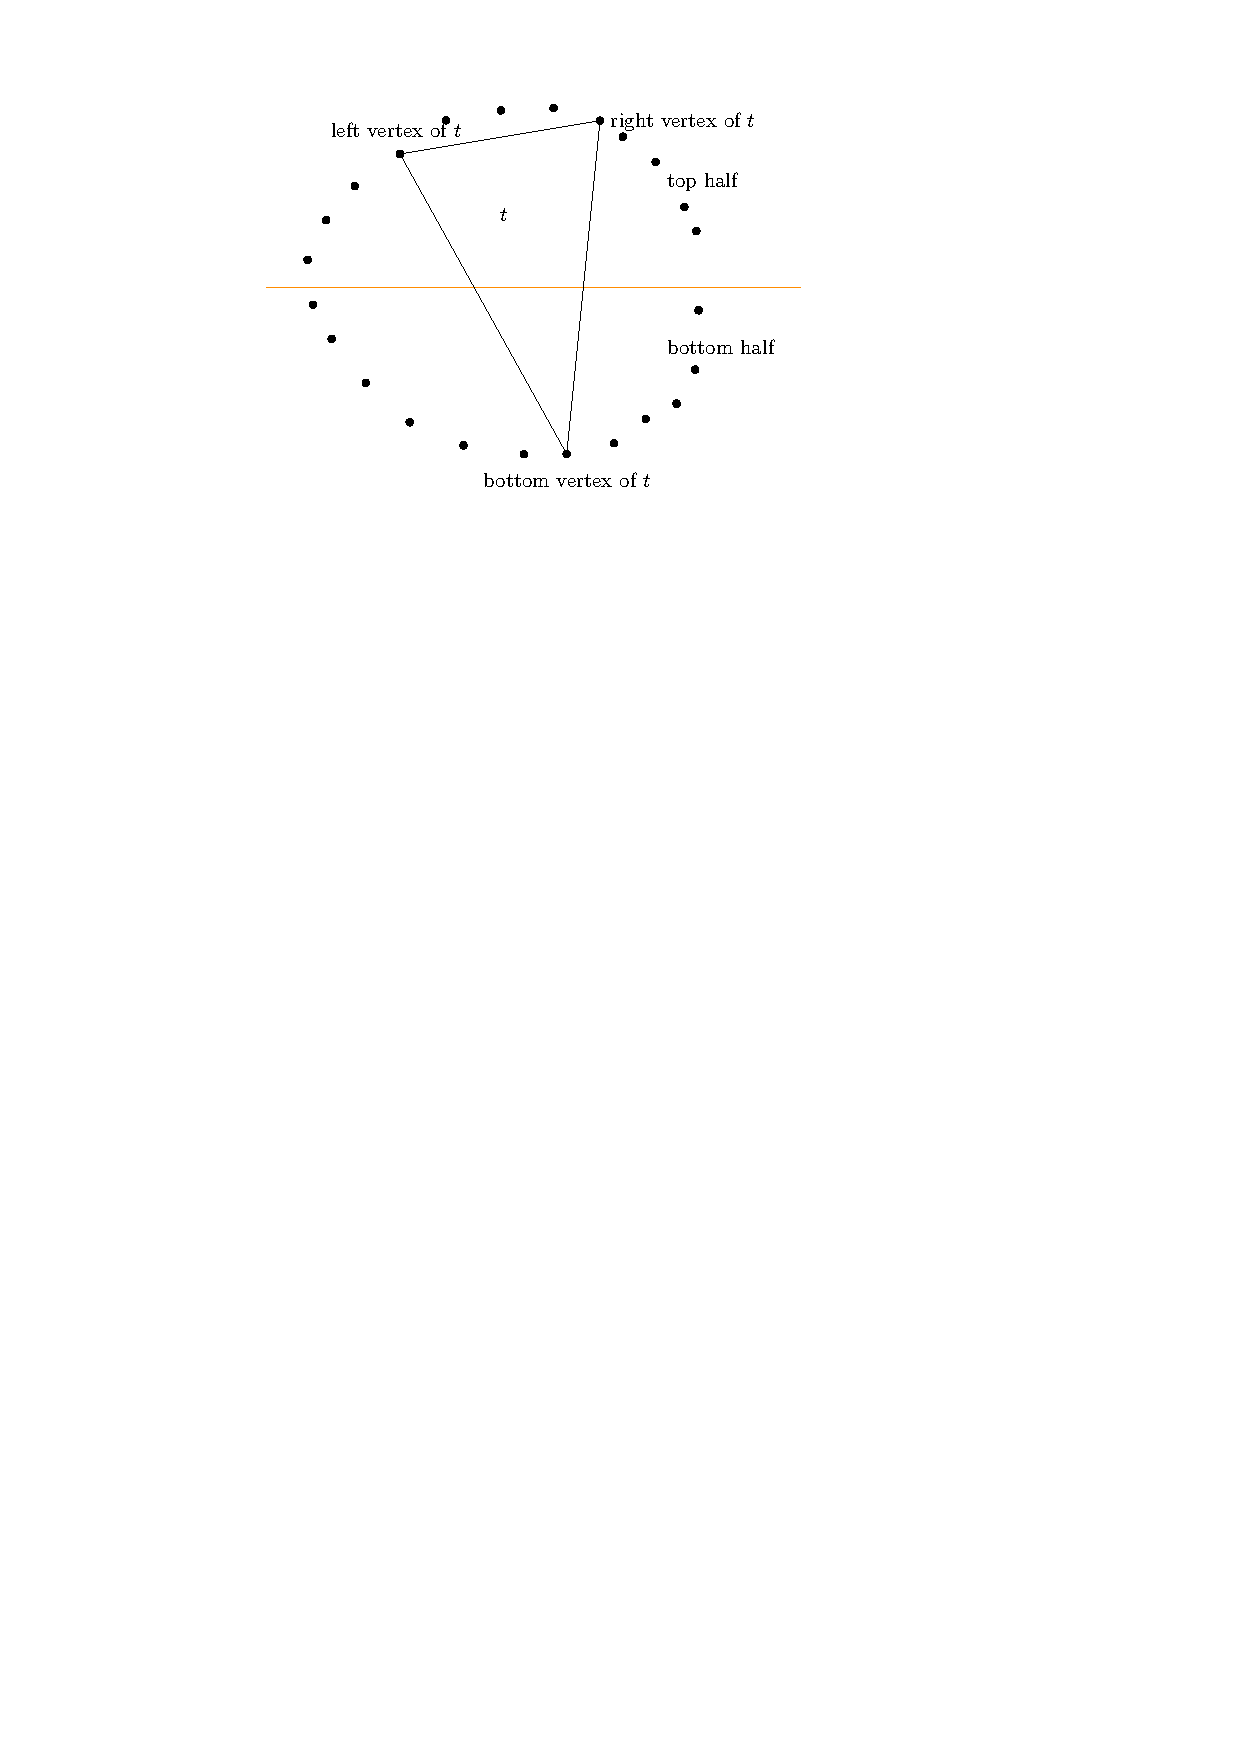
\includegraphics{figs/left-right}
  \end{center}
  \caption{$\ex'$ only counts triangles with two vertices in the top half
     and one vertex in the bottom half.}
  \figlabel{top-bottom}
\end{figure}

The following lemma shows that we can, without losing much, study $\ex'(n,X)$ instead of $\ex(n,X)$.

\begin{lem}\lemlabel{top-bottom}
  If $\ex'(n,X)\in O(n^c)$, then
\[
   \ex(n,X)\in 
      \begin{cases} 
          O(n^c)     & \text{if $c>1$} \\
          O(n\log n) & \text{if $c=1$}
      \end{cases}
\]
\end{lem}

\begin{proof}
   Let $S$ be a set of triangles that avoids $X$.  
   Every triangle in $S$
   is of one of the following types:
   \begin{enumerate}
      \item It has one vertex in the top half and two in the bottom half; there are $O(n^{c})$ such triangles.
      \item It has two vertices in the top half and one in the bottom half; there are $O(n^{c})$ such triangles.
      \item It has all three vertices in the top half; there are at most $\ex(\lfloor n/2\rfloor,X)$ such triangles.
      \item It has all three vertices in the bottom half; there are at most $\ex(\lceil n/2\rceil,X)$ such triangles.
   \end{enumerate}
   Thus, we obtain the recurrence inequality:
   \[  \ex(n,X) = O(n^{c}) + \ex(\lfloor n/2\rfloor,X) + \ex(\lceil n/2\rceil,X) \]
   which resolves to $O(n^c)$ for $c>1$ and $O(n\log n)$ for $c=1$.
\end{proof}


\subsection{The Dot Puzzle View}

It is sometimes helpful to take the top/bottom view of the problem
and turn it, instead, into a puzzle.  Refer to \figref{point-view}.
In this puzzle, we are given $\binom{n}{2}$ points,
\[
    Q = \{(x,y): y\in\{1,\ldots,n-1\}, x\in\{y+1,\ldots,n-1\} \} \enspace .
\]
These points model the top/bottom view on a set of size $2n$, where the
point $(x,y)$ represents a triangle whose vertices are some point on
the bottom and the $x$th and $y$th points on the top, where the top
vertices are labelled $1,\ldots,n$ from left to right.

\begin{figure}
   \begin{center}
      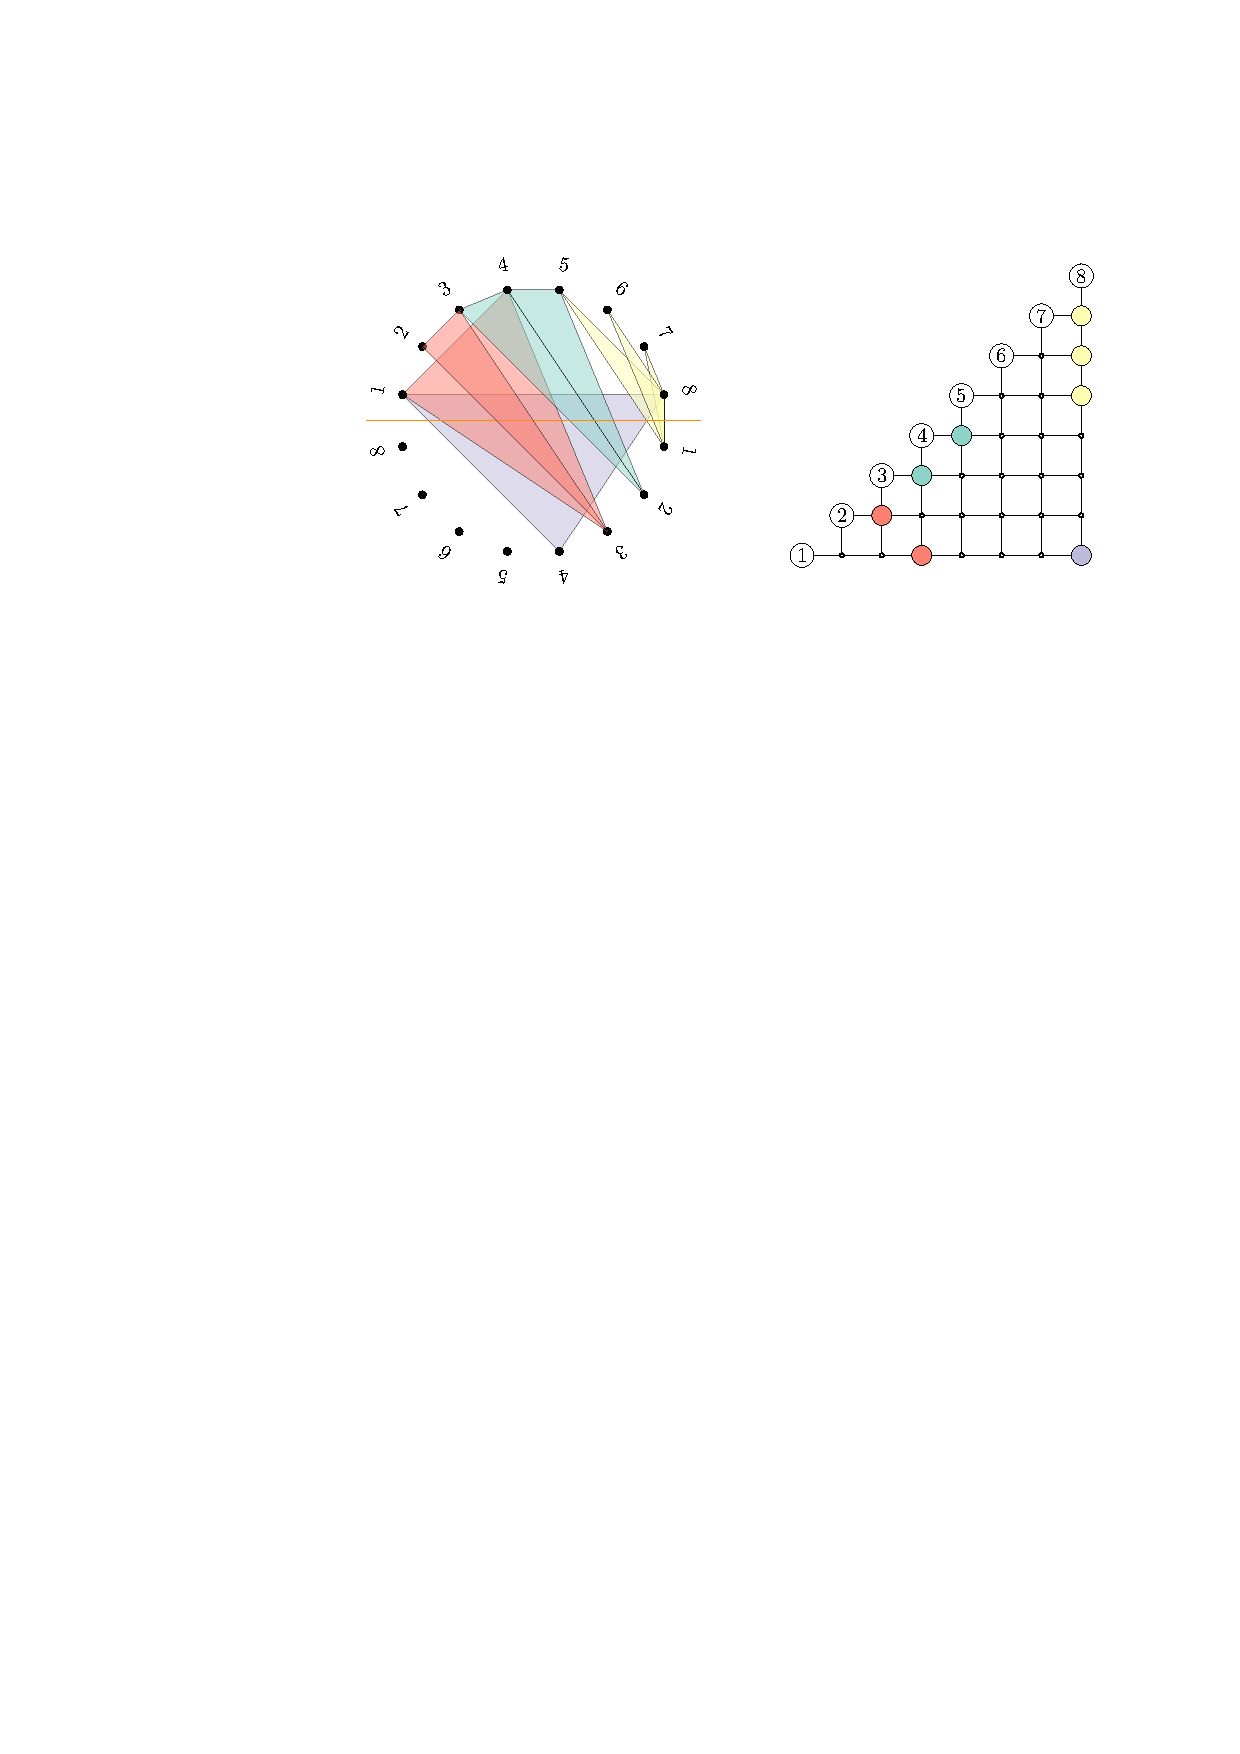
\includegraphics{figs/point-view}
   \end{center}
   \caption{The Dot Puzzle View of the Top/Bottom View. Orange points were
     selected in round 1, green points in round 2 and pink points in round 3.}
   \figlabel{point-view}
\end{figure}

The dot-puzzle proceeds in $n$ rounds and during the $i$th round, the
player selects a set $Q_i\subseteq Q$ subject to certain constraints
that depend on the points selected in rounds $1,\ldots,i-1$.  In the
top/bottom view, the $i$th round determines which pairs of top vertices
form a triangle with the $i$th bottom vertex, where the bottom
vertices are labelled $1,\ldots,n$ from right to left.  

Of course, the constraints on which points can be selected during round
$i$ depend on the set of forbidden configurations and $\bigcup_{j=1}^{i-1}
Q_i$.  By proving upper or lower bounds on $\sum_{i=1}^n |Q_i|$ we obtain
bounds on the maximum number of triangles obtained in the top-bottom view.

\Tabref{forbidden} summarizes the constraints on the puzzle induced by
various forbidden configurations.  The left column shows the forbidden
configuration.  The middle column describes what happens in subsequent
rounds when the large black point is placed during a round; none of
the points marked with red crosses can be used in subsequent rounds.
The right column shows what happens during the same round; none of the
points marked with red crosses can be selected during the same round.

%One caveat worth noting is that, unless $\edgea$ is a forbidden
%configuration, the same point can be chosen in different rounds.

\begin{table}
\begin{center}
\begin{tabular}{m{1ex}|>{\centering\arraybackslash}m{.45\textwidth}|>{\centering\arraybackslash}m{.45\textwidth}}
      & killed by $(x,y)$ in later rounds 
         & killed by $(x,y)$ in current round \\ \hline
$\edgeb$ & 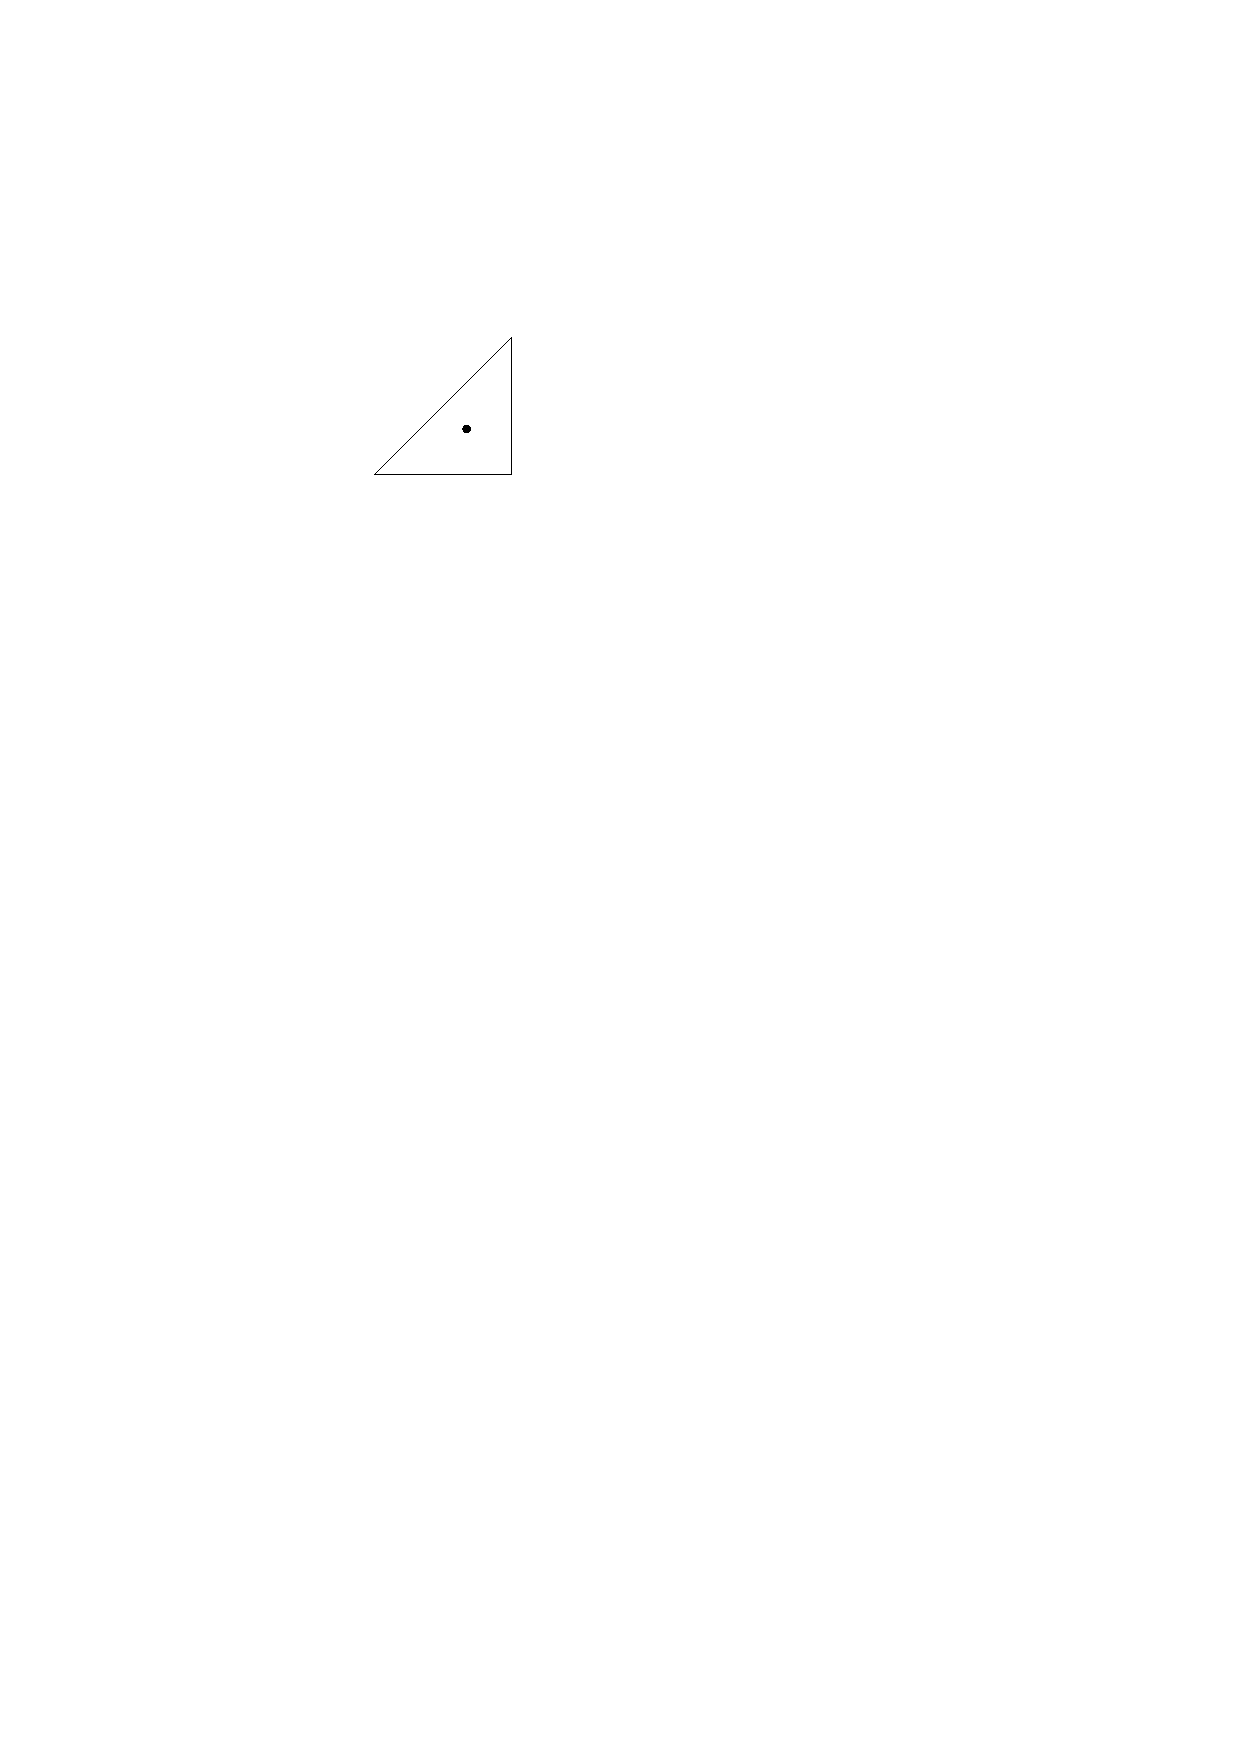
\includegraphics[scale=.8]{figs/killers-1} \break% 
           $\{\}$  
         & 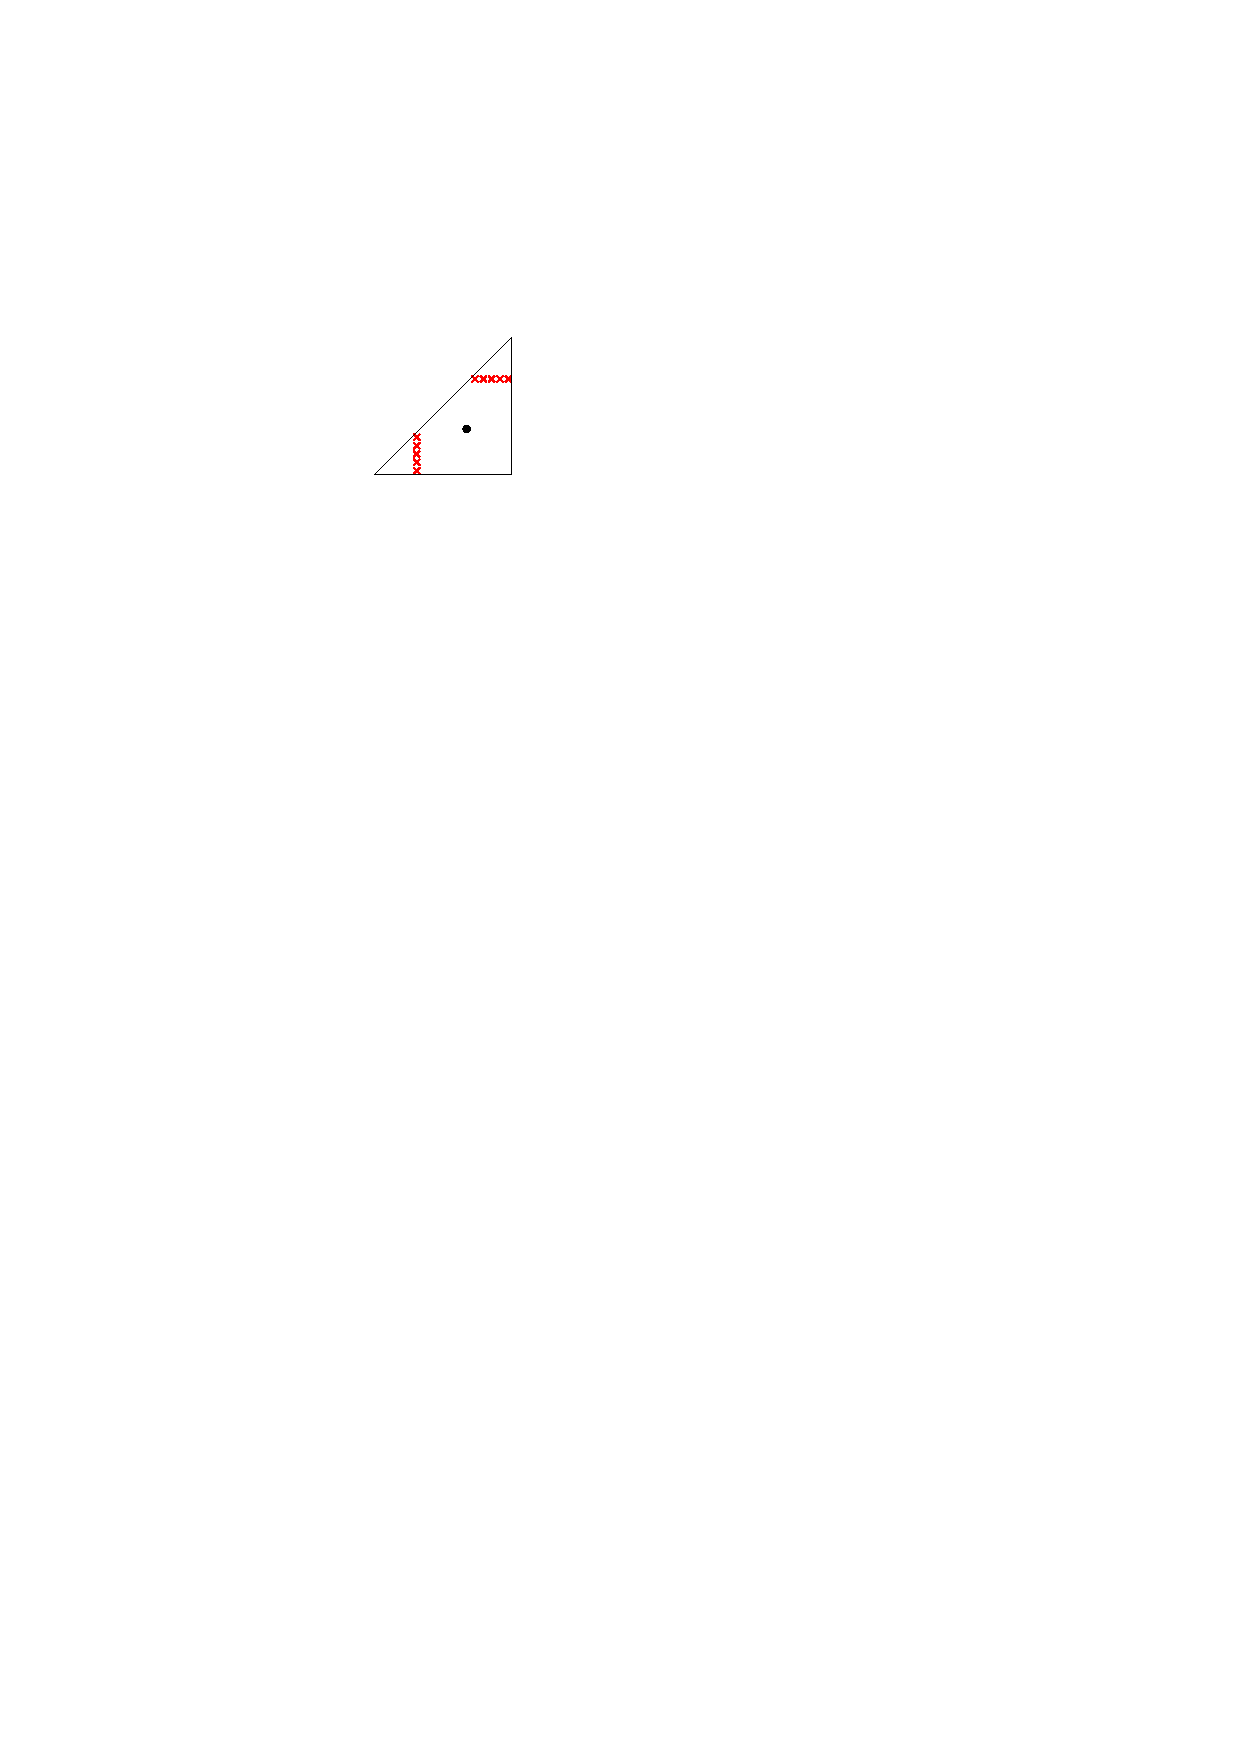
\includegraphics[scale=.8]{figs/killersb-1} \break% 
           $\{(x',x)\} \cup \{(y,y')\}$ \\ 
$\edgea$ & 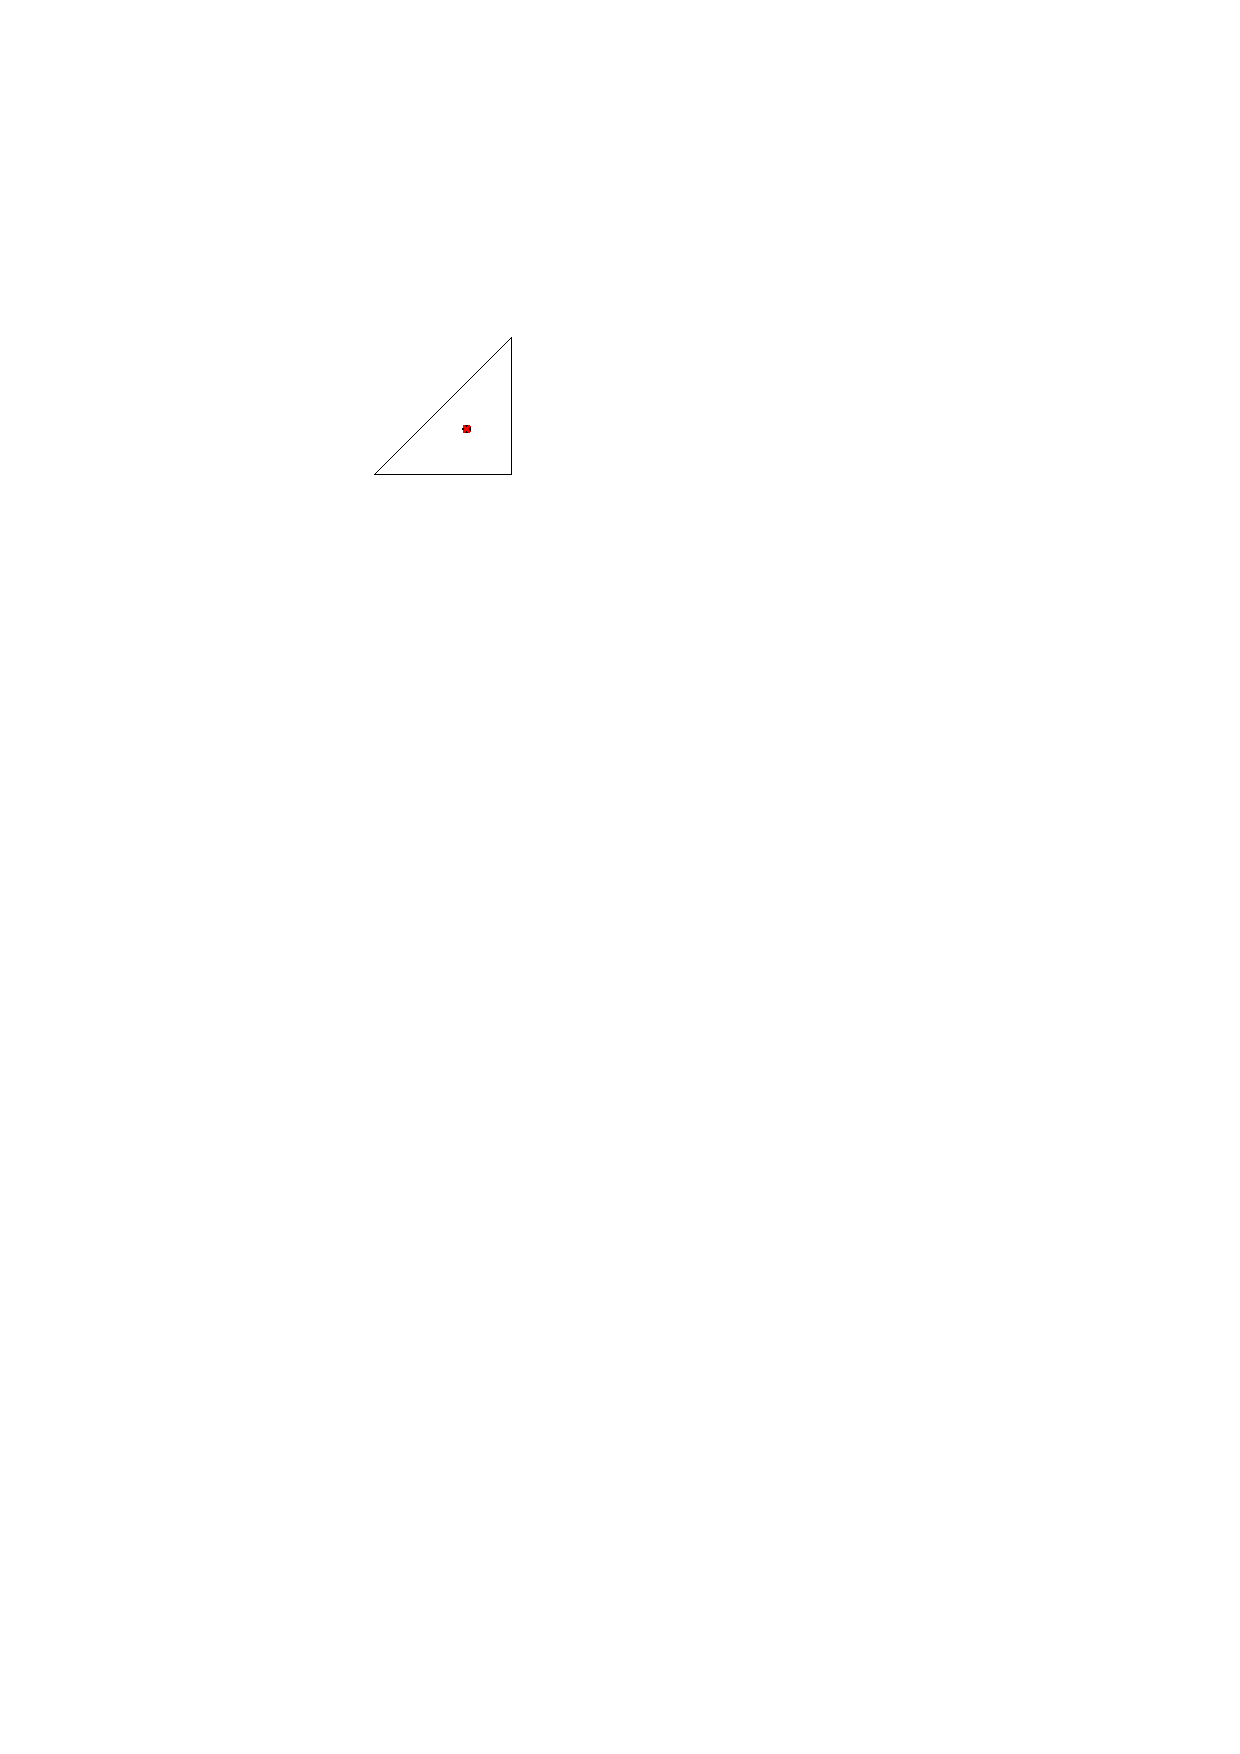
\includegraphics[scale=.8]{figs/killers-2} \break% 
           $\{(x,y)\}$ 
         & 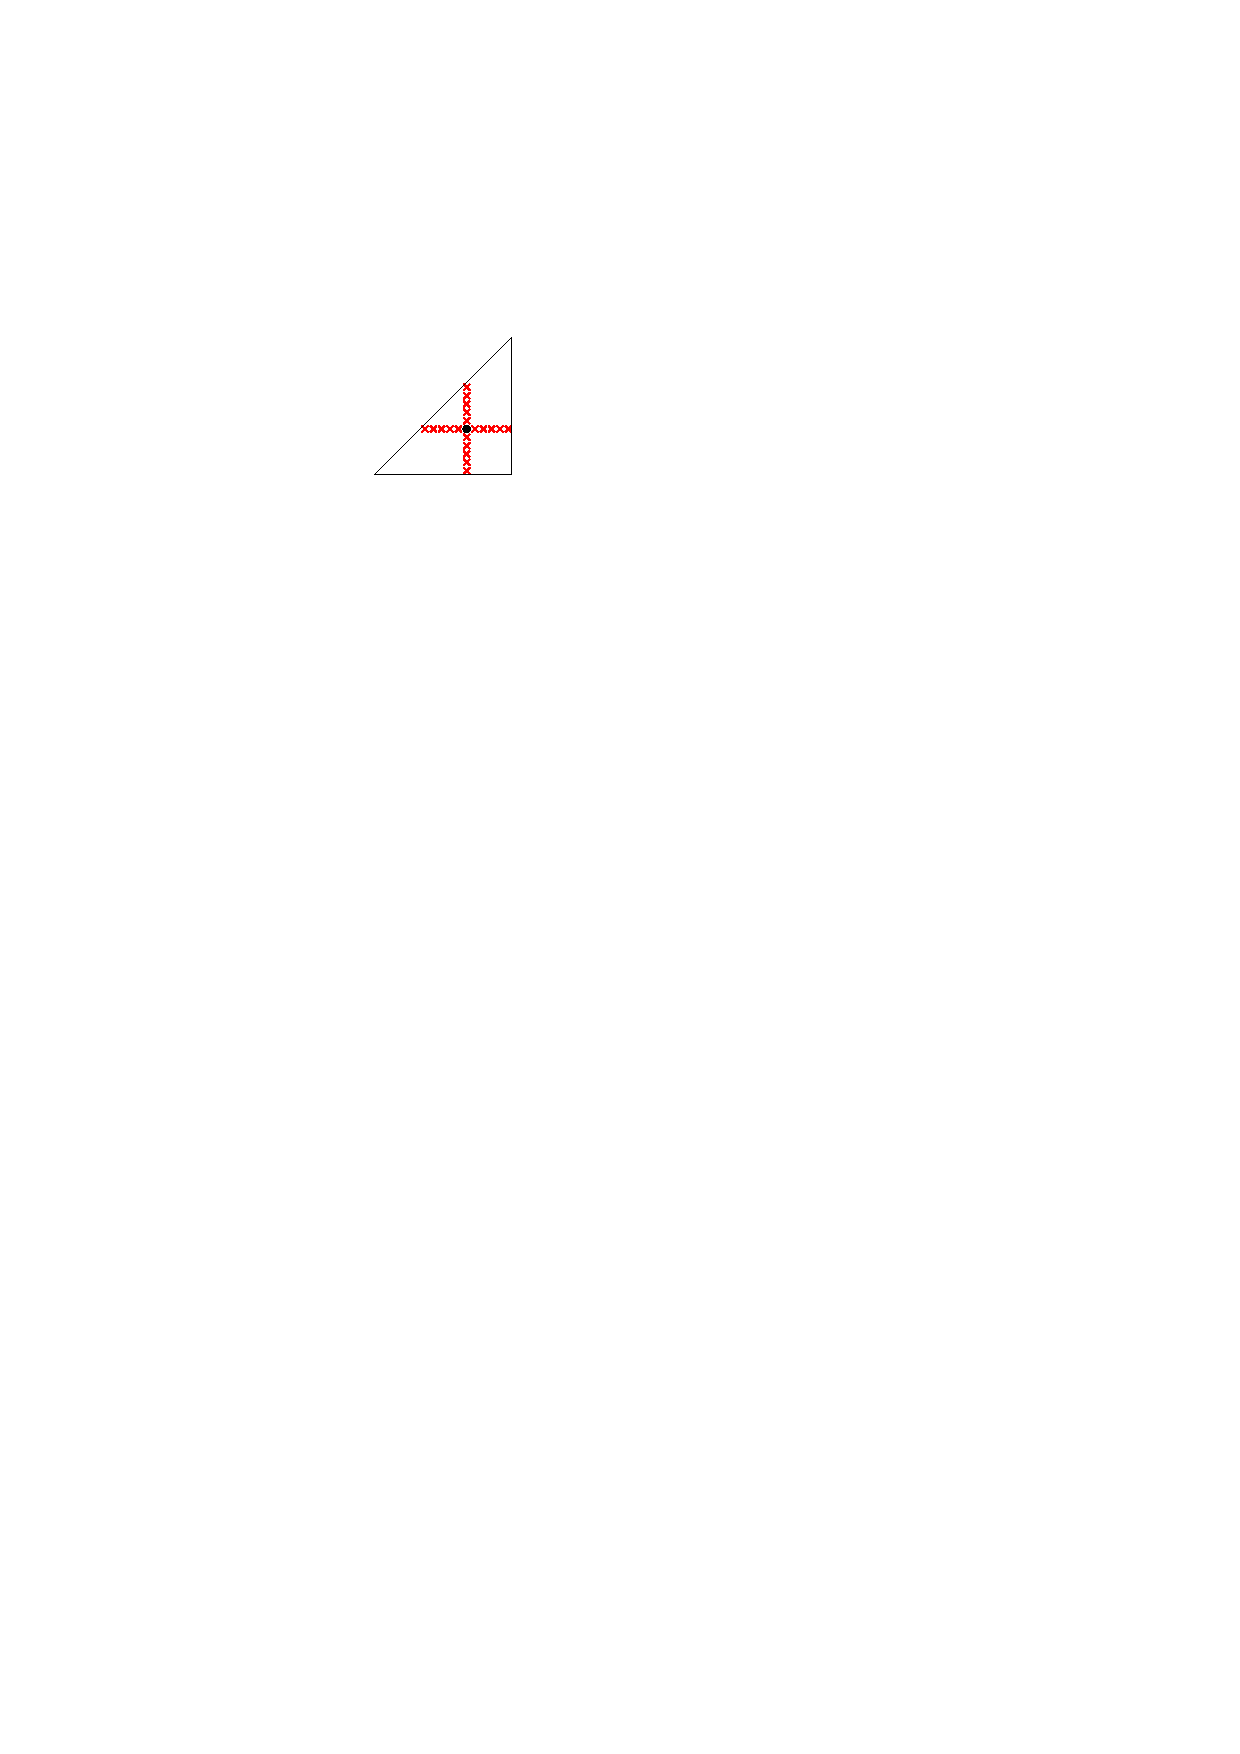
\includegraphics[scale=.8]{figs/killersb-2} \break% 
           $\{(x,y')\} \cup \{(x',y)\}$ \\
$\vertexa$ & 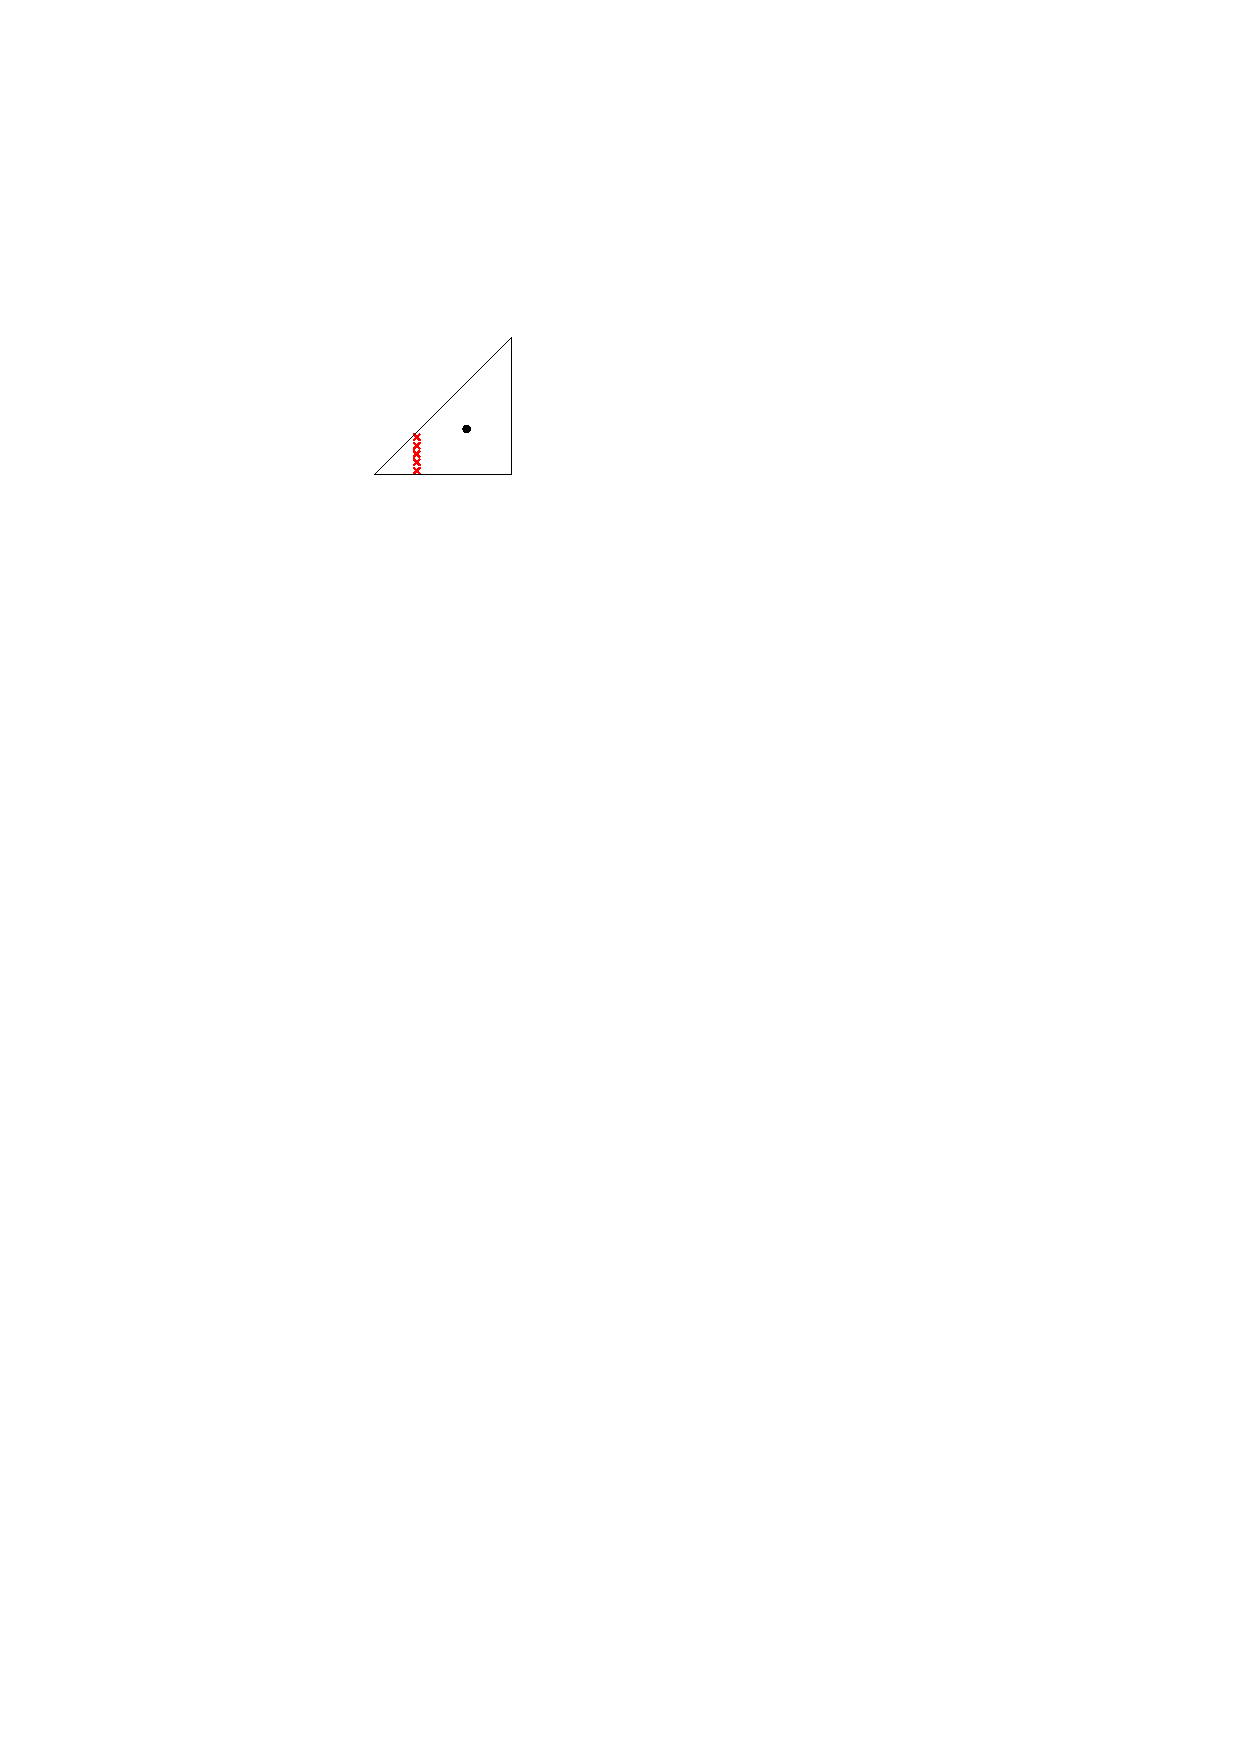
\includegraphics[scale=.8]{figs/killers-3} \break% 
             $\{(x',y) : x'<x \}\cup\{(x,y') : y'<y \}$ 
           & 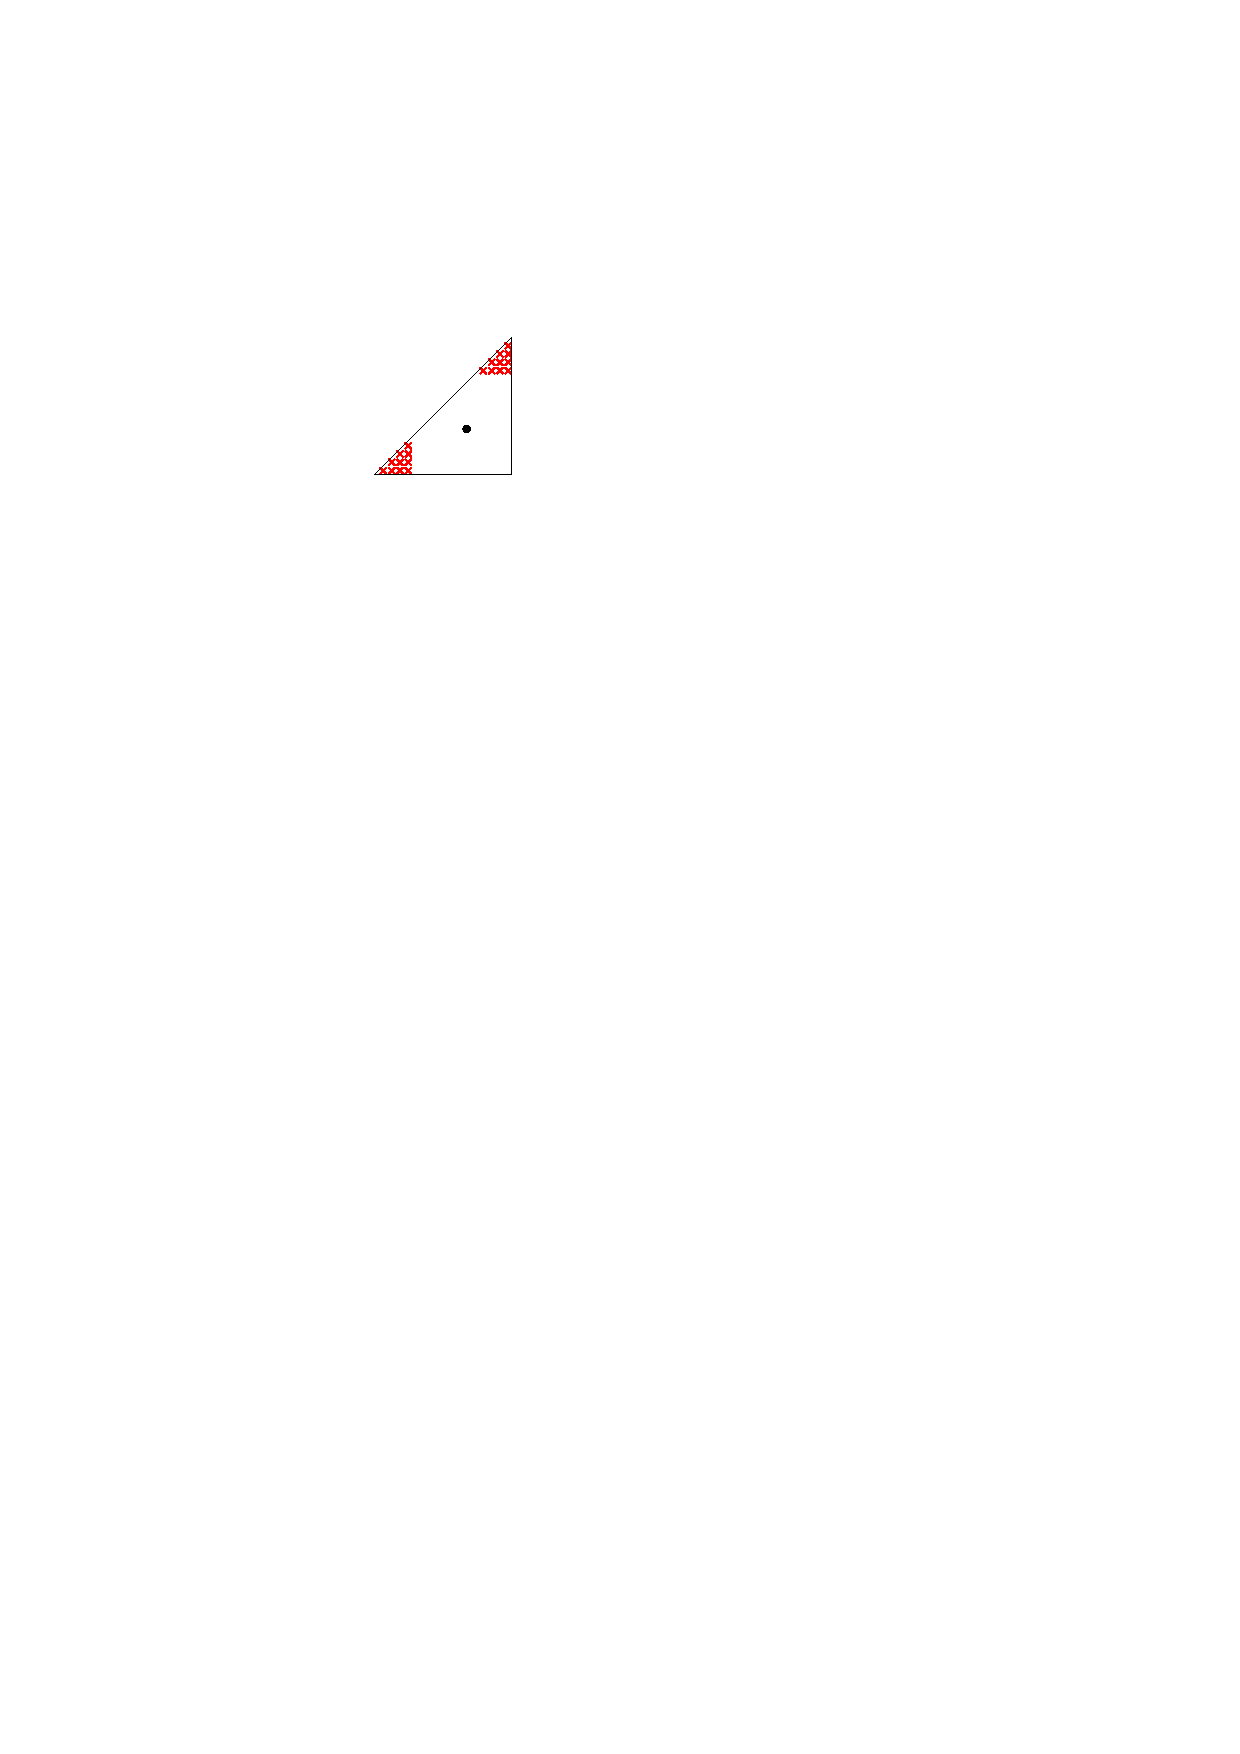
\includegraphics[scale=.8]{figs/killersb-3} \break%
             $\{(x',y'): x' < y\text{ or } y'> x\}$ \\
$\vertexb$ &  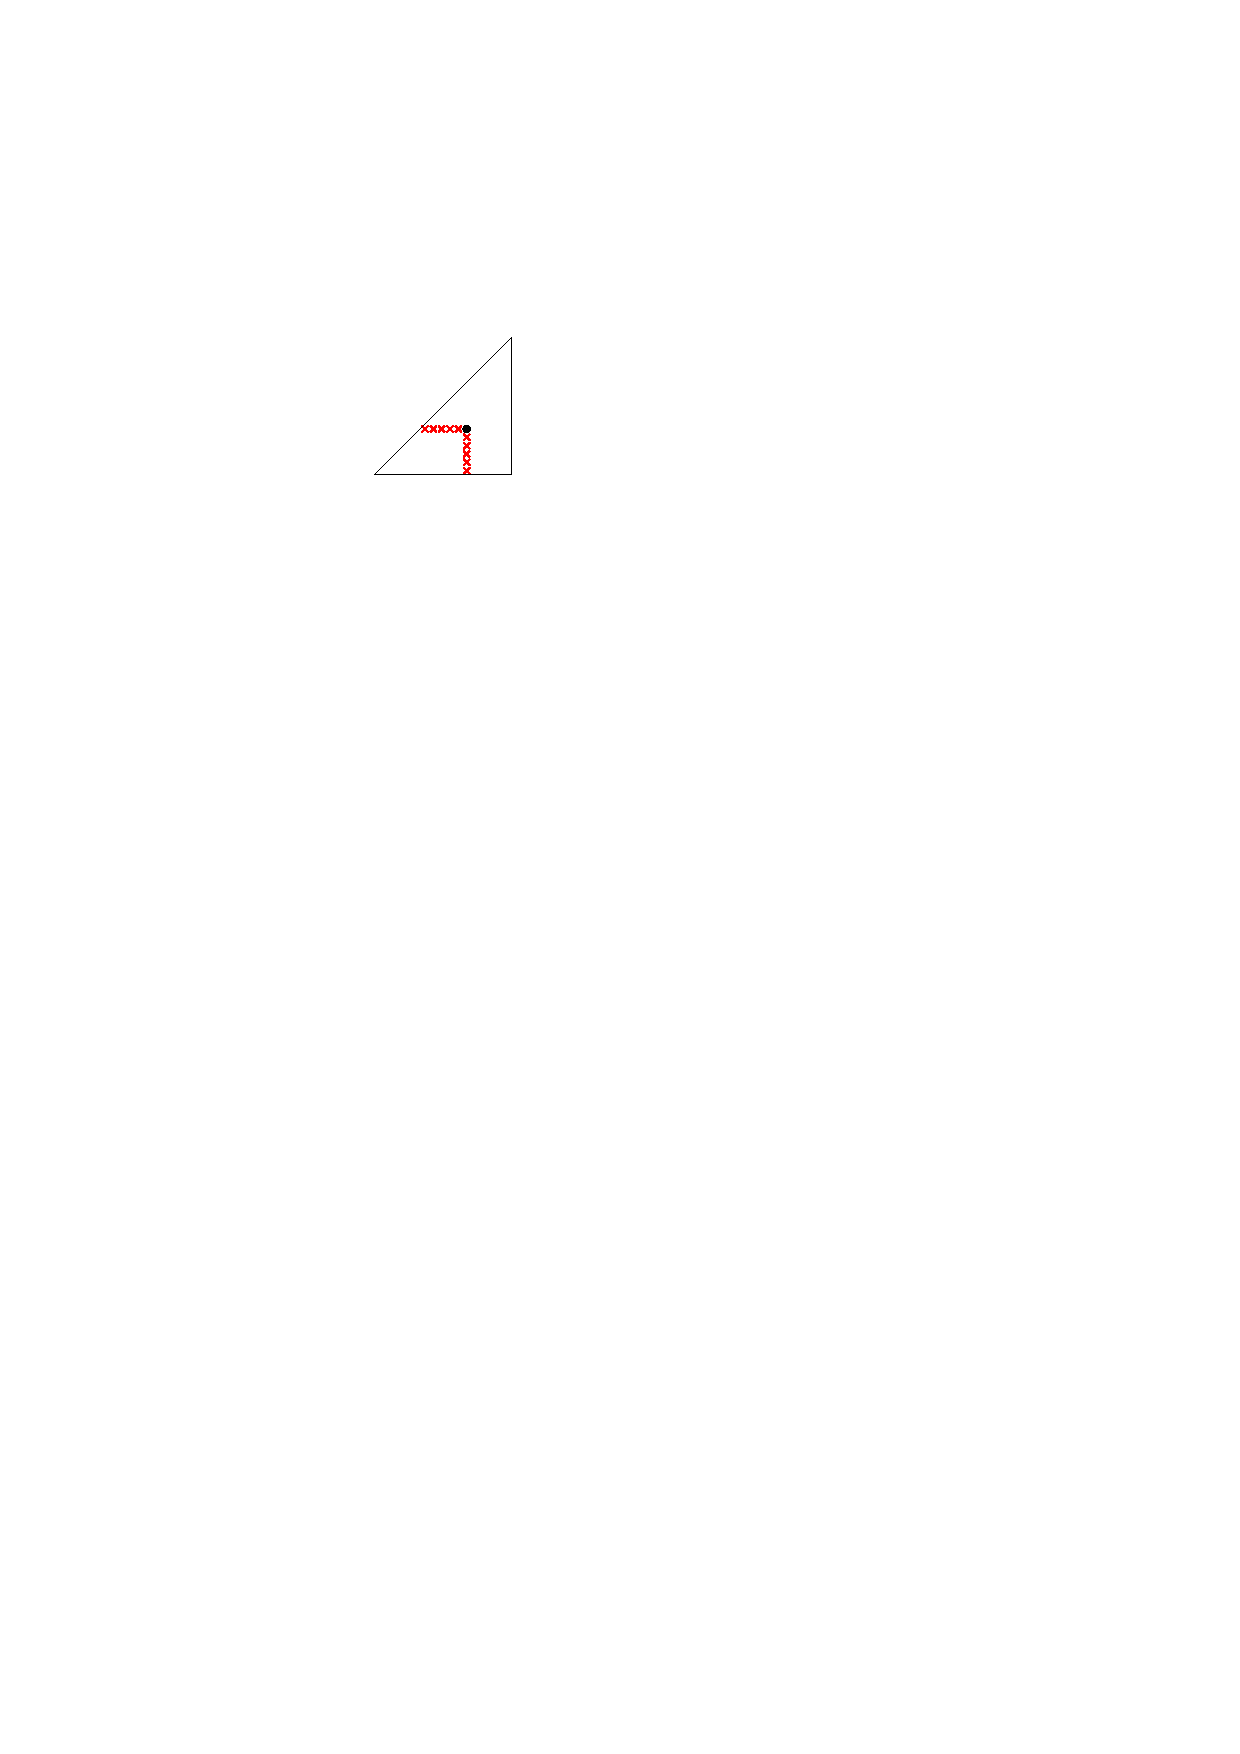
\includegraphics[scale=.8]{figs/killers-4} \break%
              $\{(x',y) : x'<x \}\cup\{(x,y') : y'<y \}$ 
         &  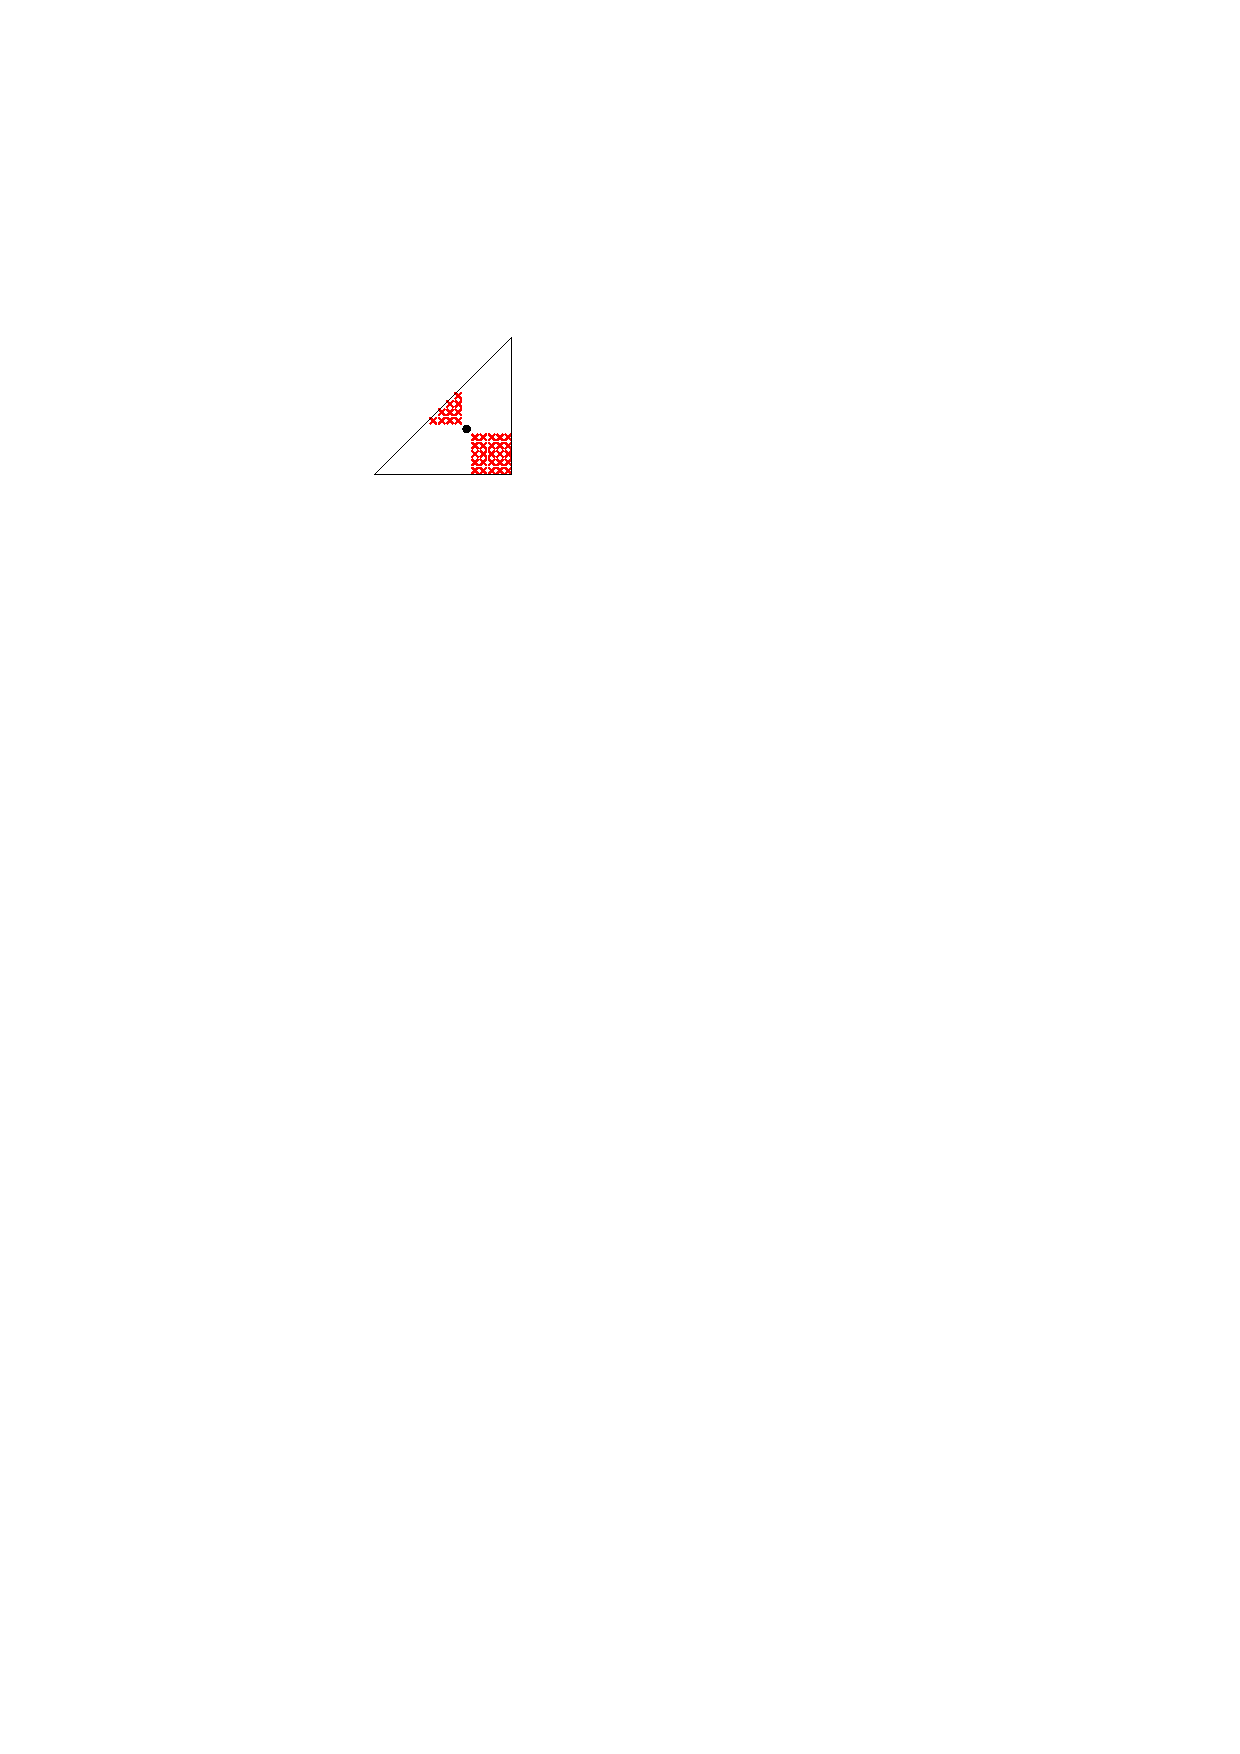
\includegraphics[scale=.8]{figs/killersb-4} \break%
            $\{(x',y'):\sign(x'-x)=\sign(y-y')\}$ \\
$\vertexc$ &  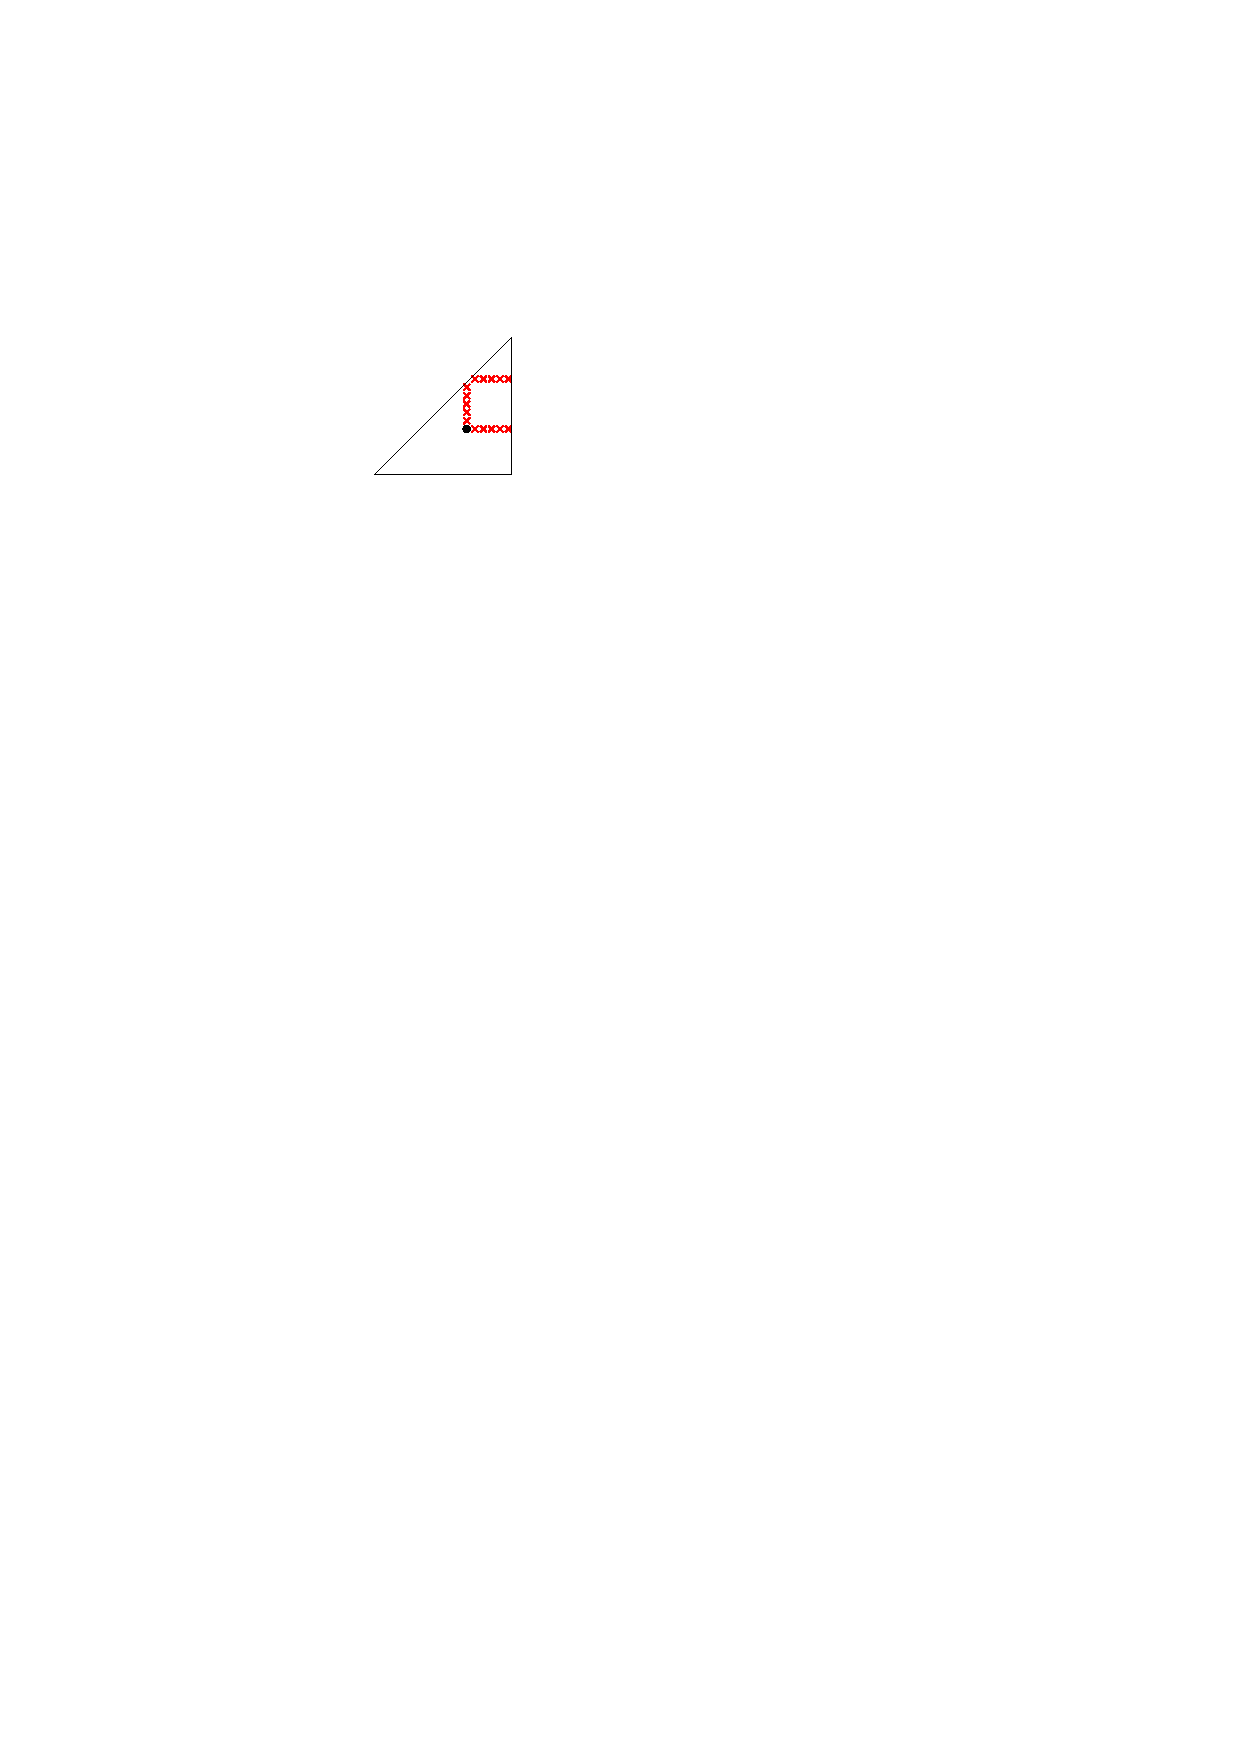
\includegraphics[scale=.8]{figs/killers-5} \break% 
              $\{(x',y) : x'>x \}\cup\{(x,y') : y'>y \}$ 
         &  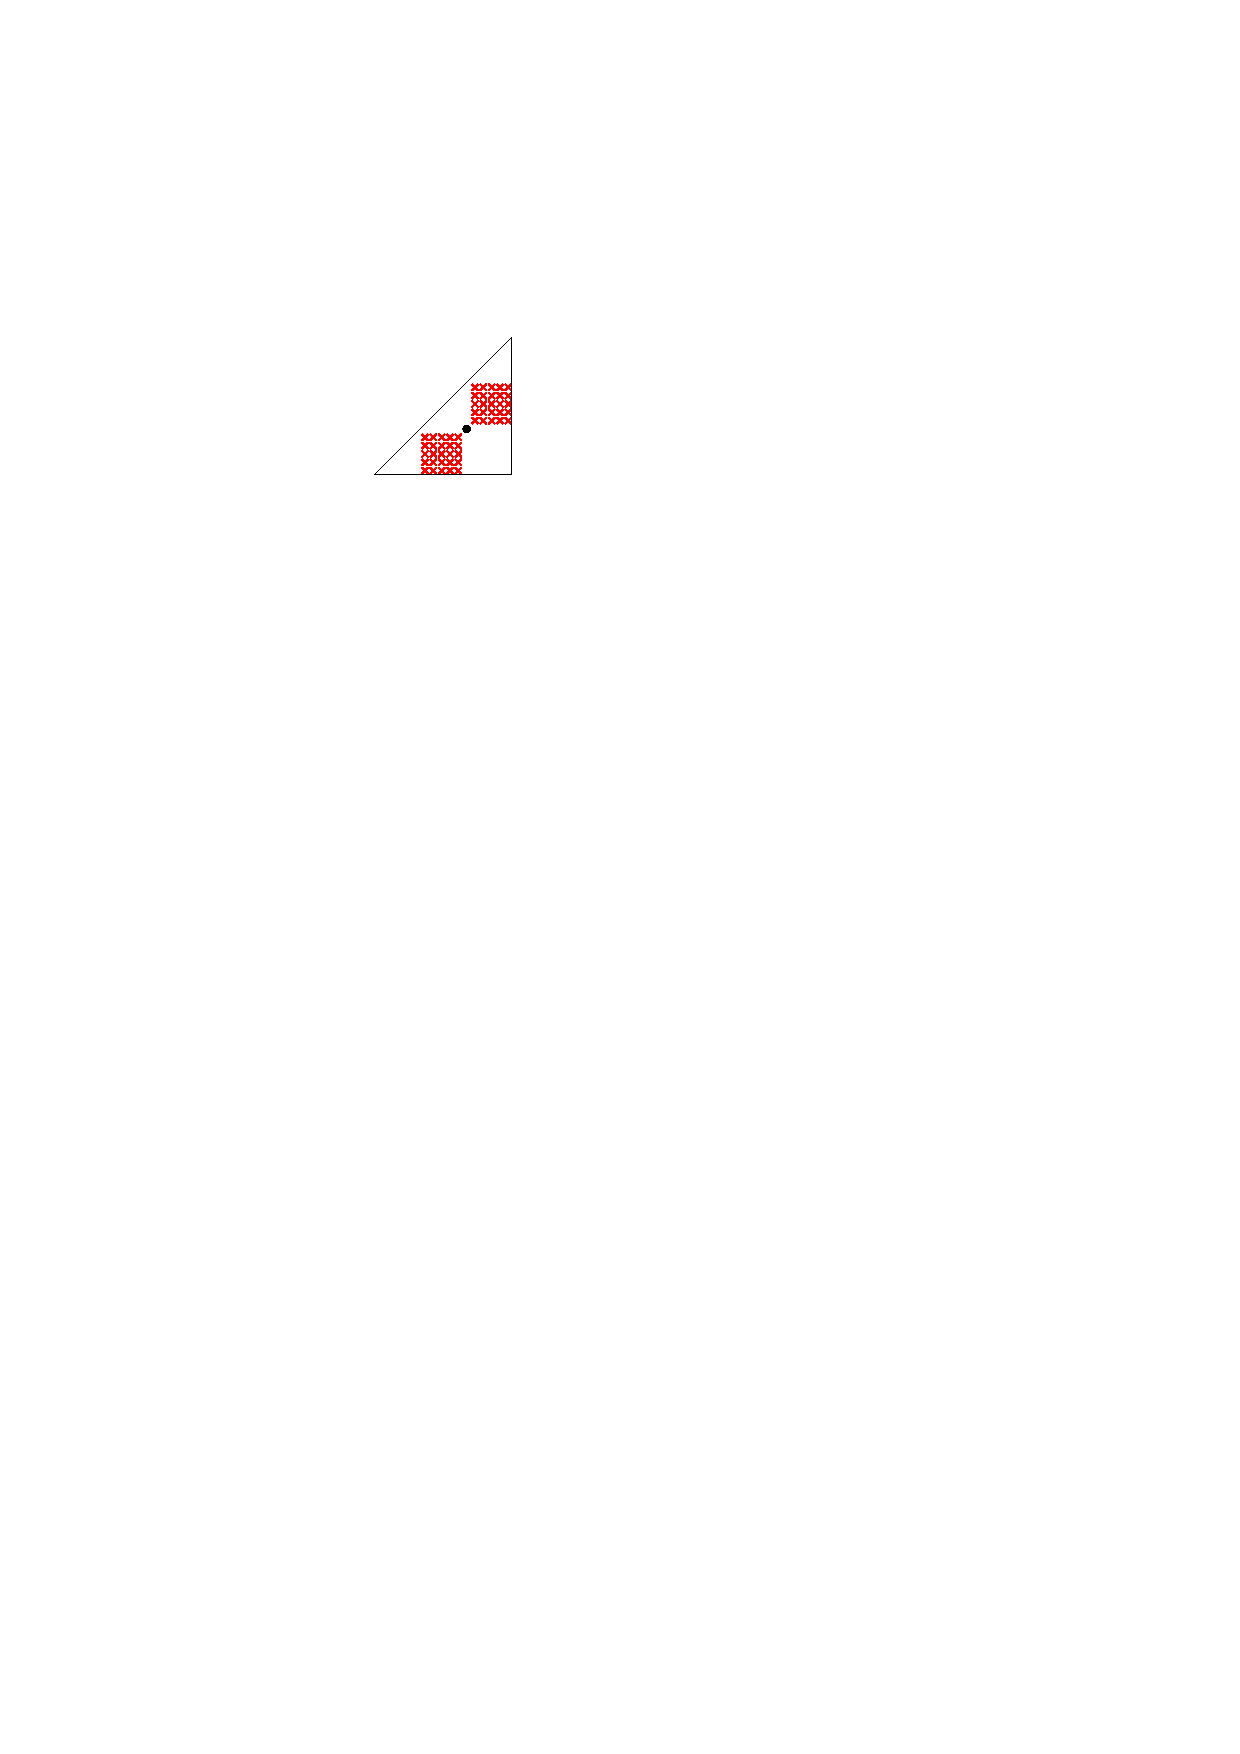
\includegraphics[scale=.8]{figs/killersb-5} \break% 
            $\{(x',y'):\sign(x'-x)=\sign(y'-y)\}$ \\
$\disjointa$ &  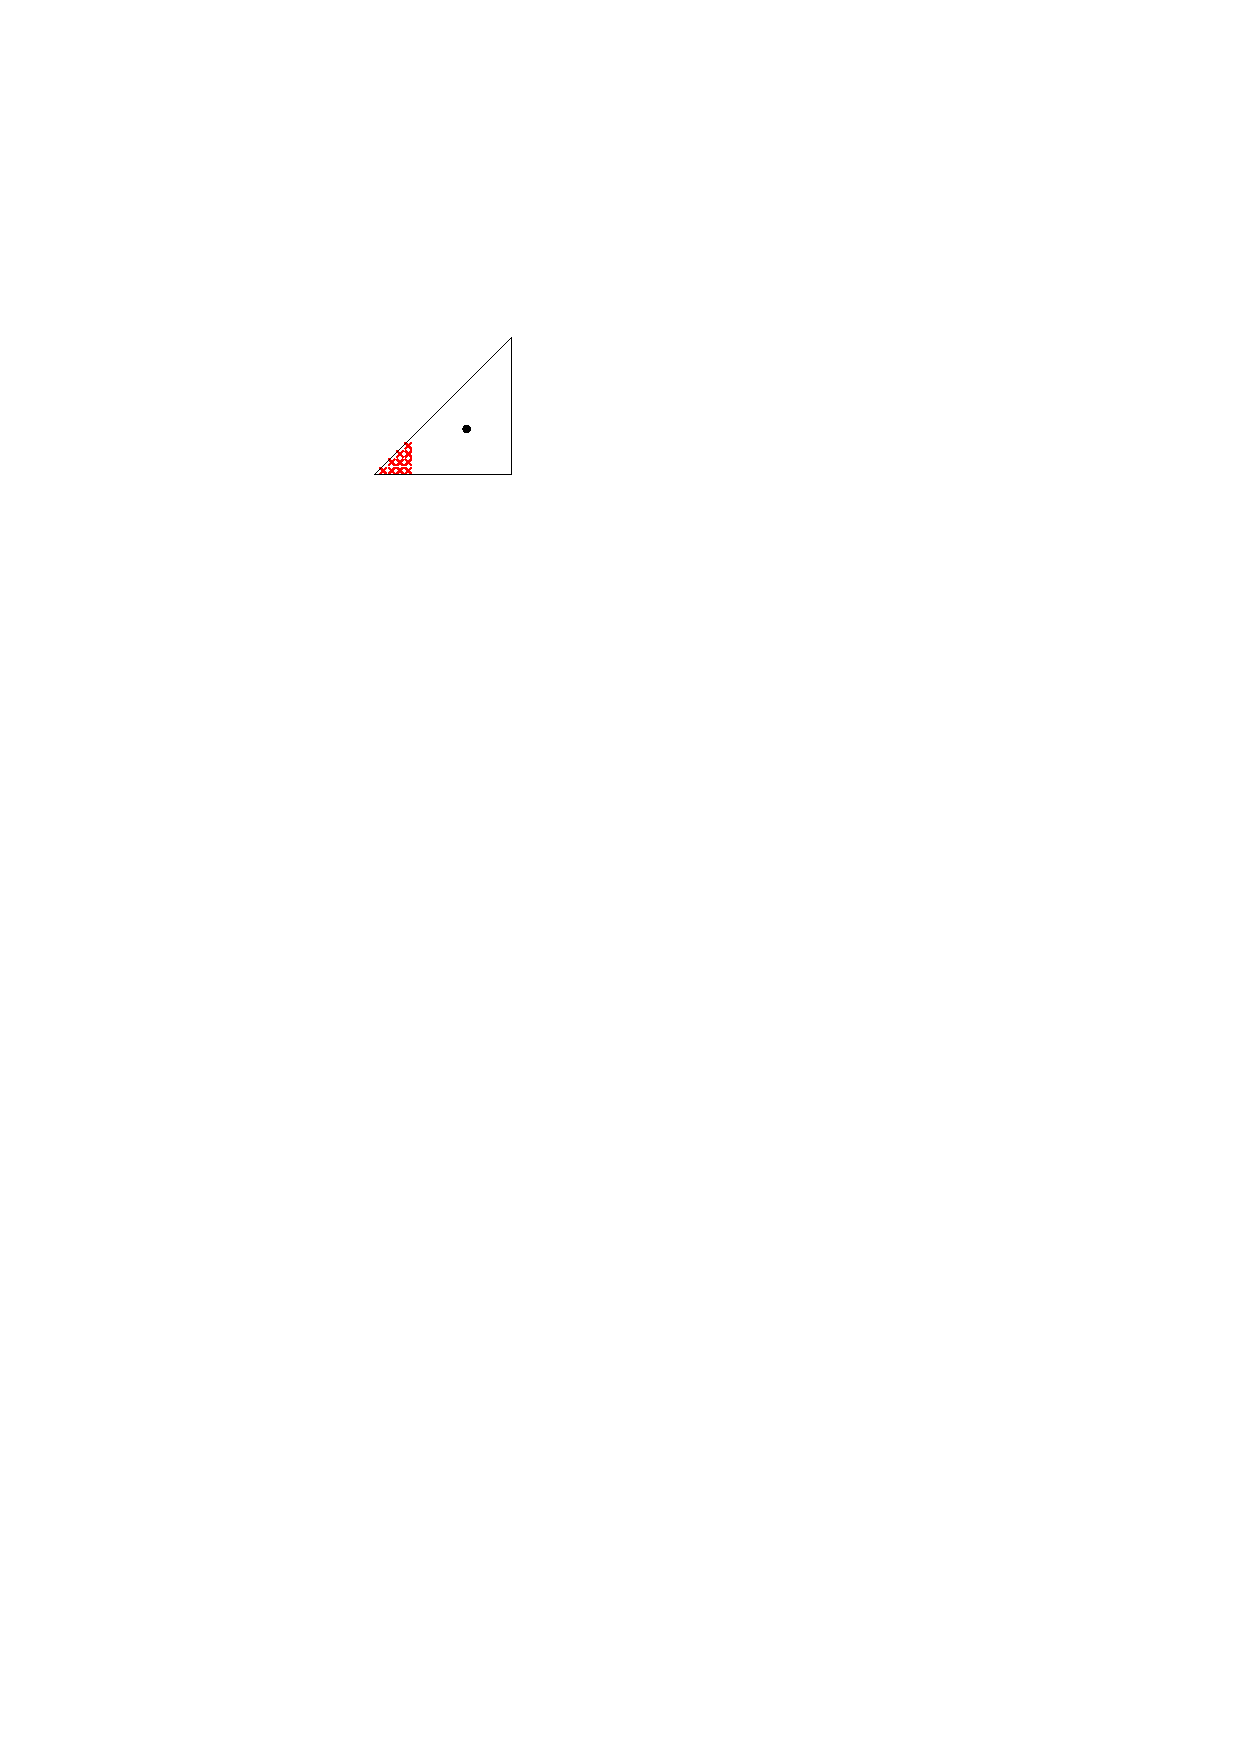
\includegraphics[scale=.8]{figs/killers-6} \break%
                $\{(x',y'): x'< y\}$
         & 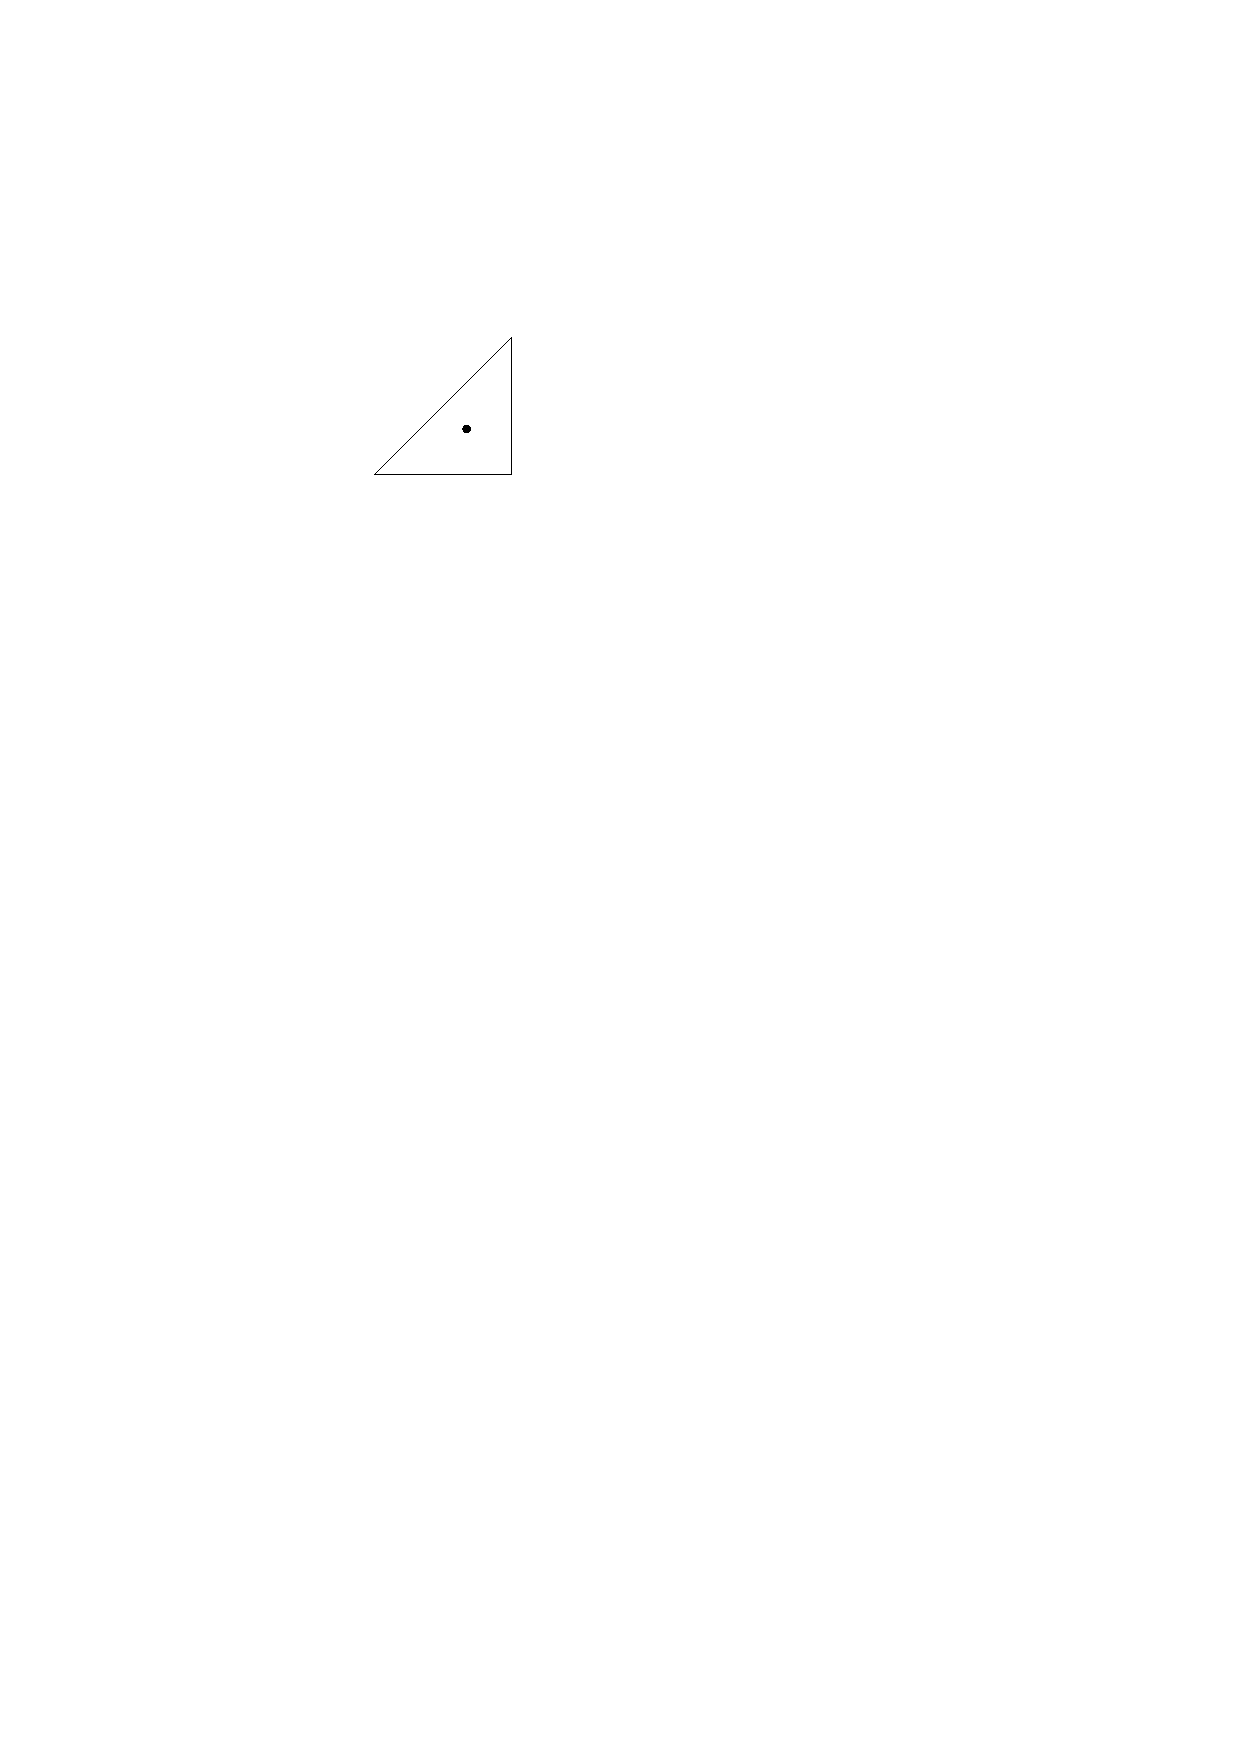
\includegraphics[scale=.8]{figs/killersb-6} \break%
           $\{\}$ \\
$\disjointb$ & 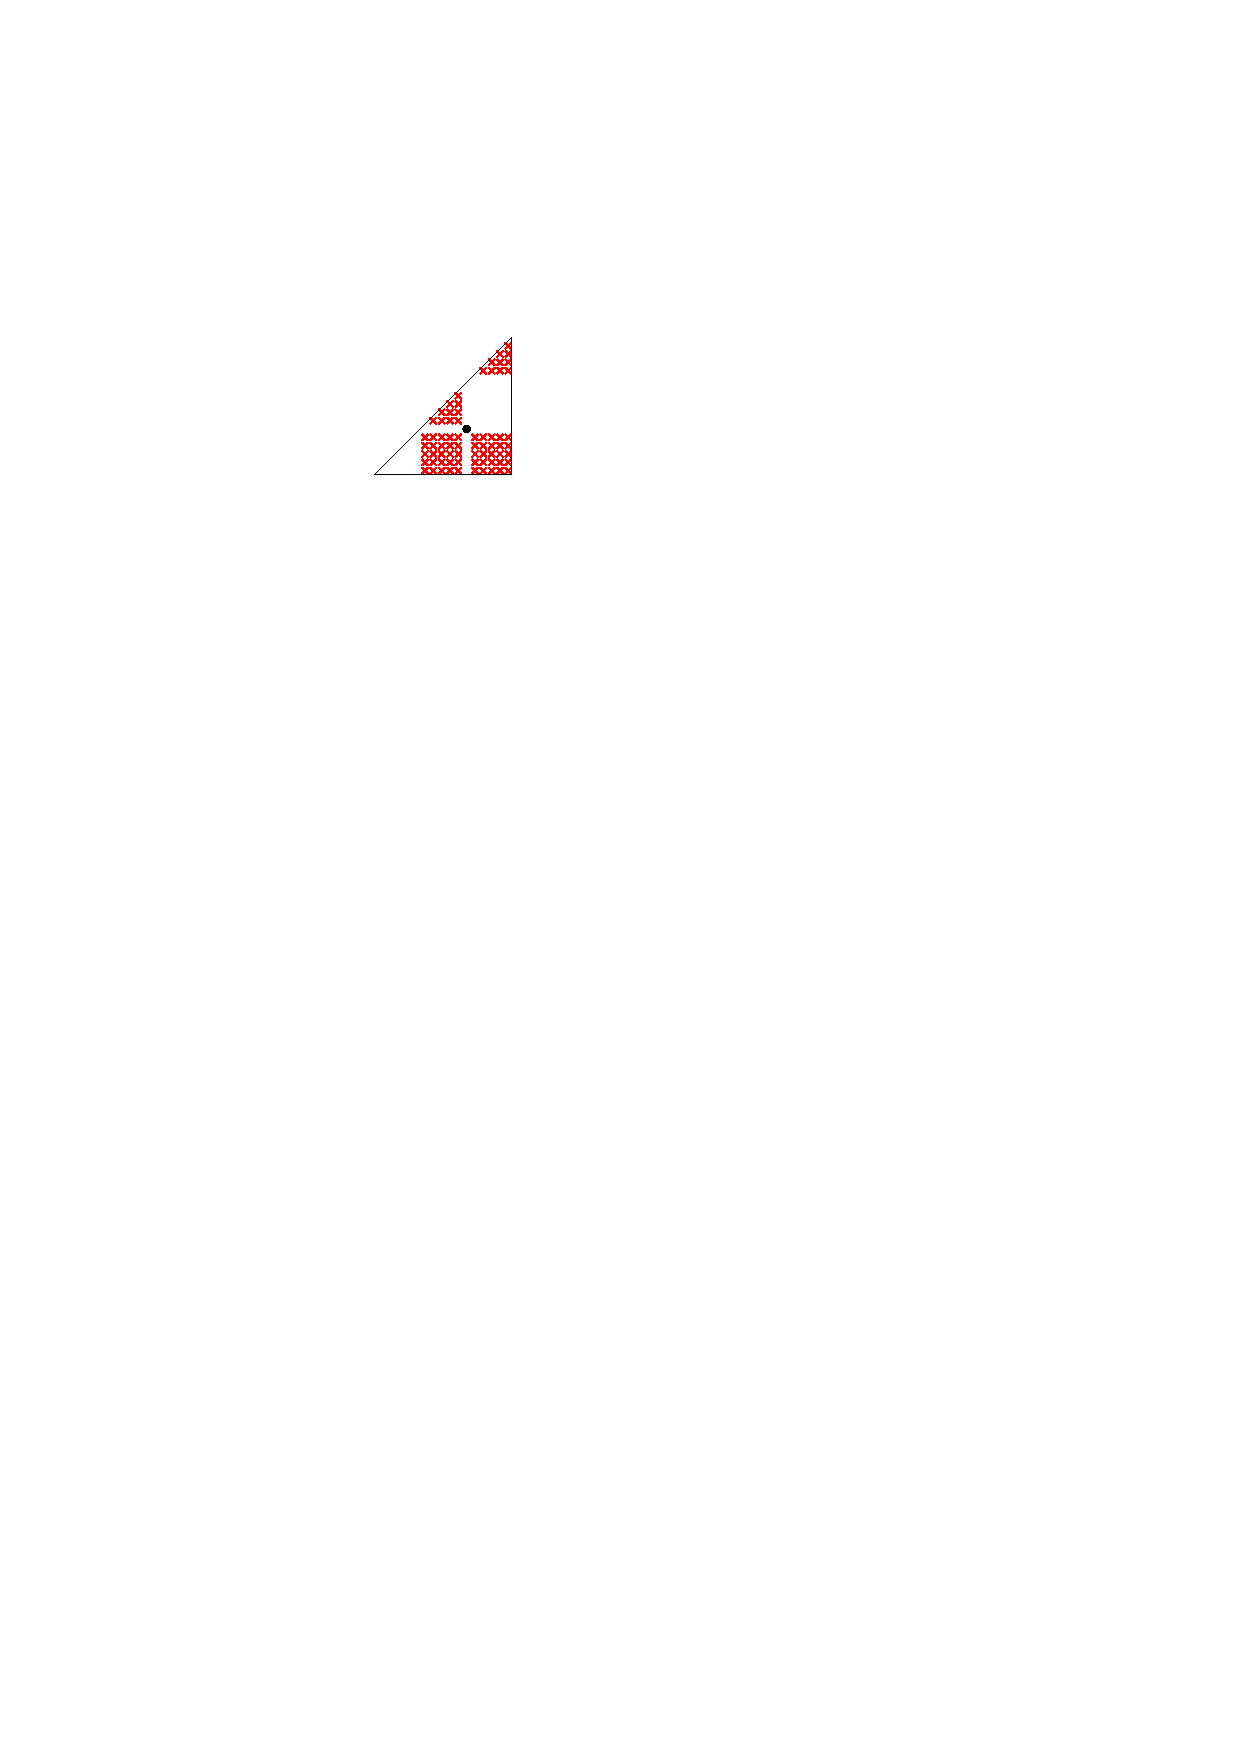
\includegraphics[scale=.8]{figs/killers-7} \break%
               $\{(x',y'): x'>x, y'< y\}$
         & 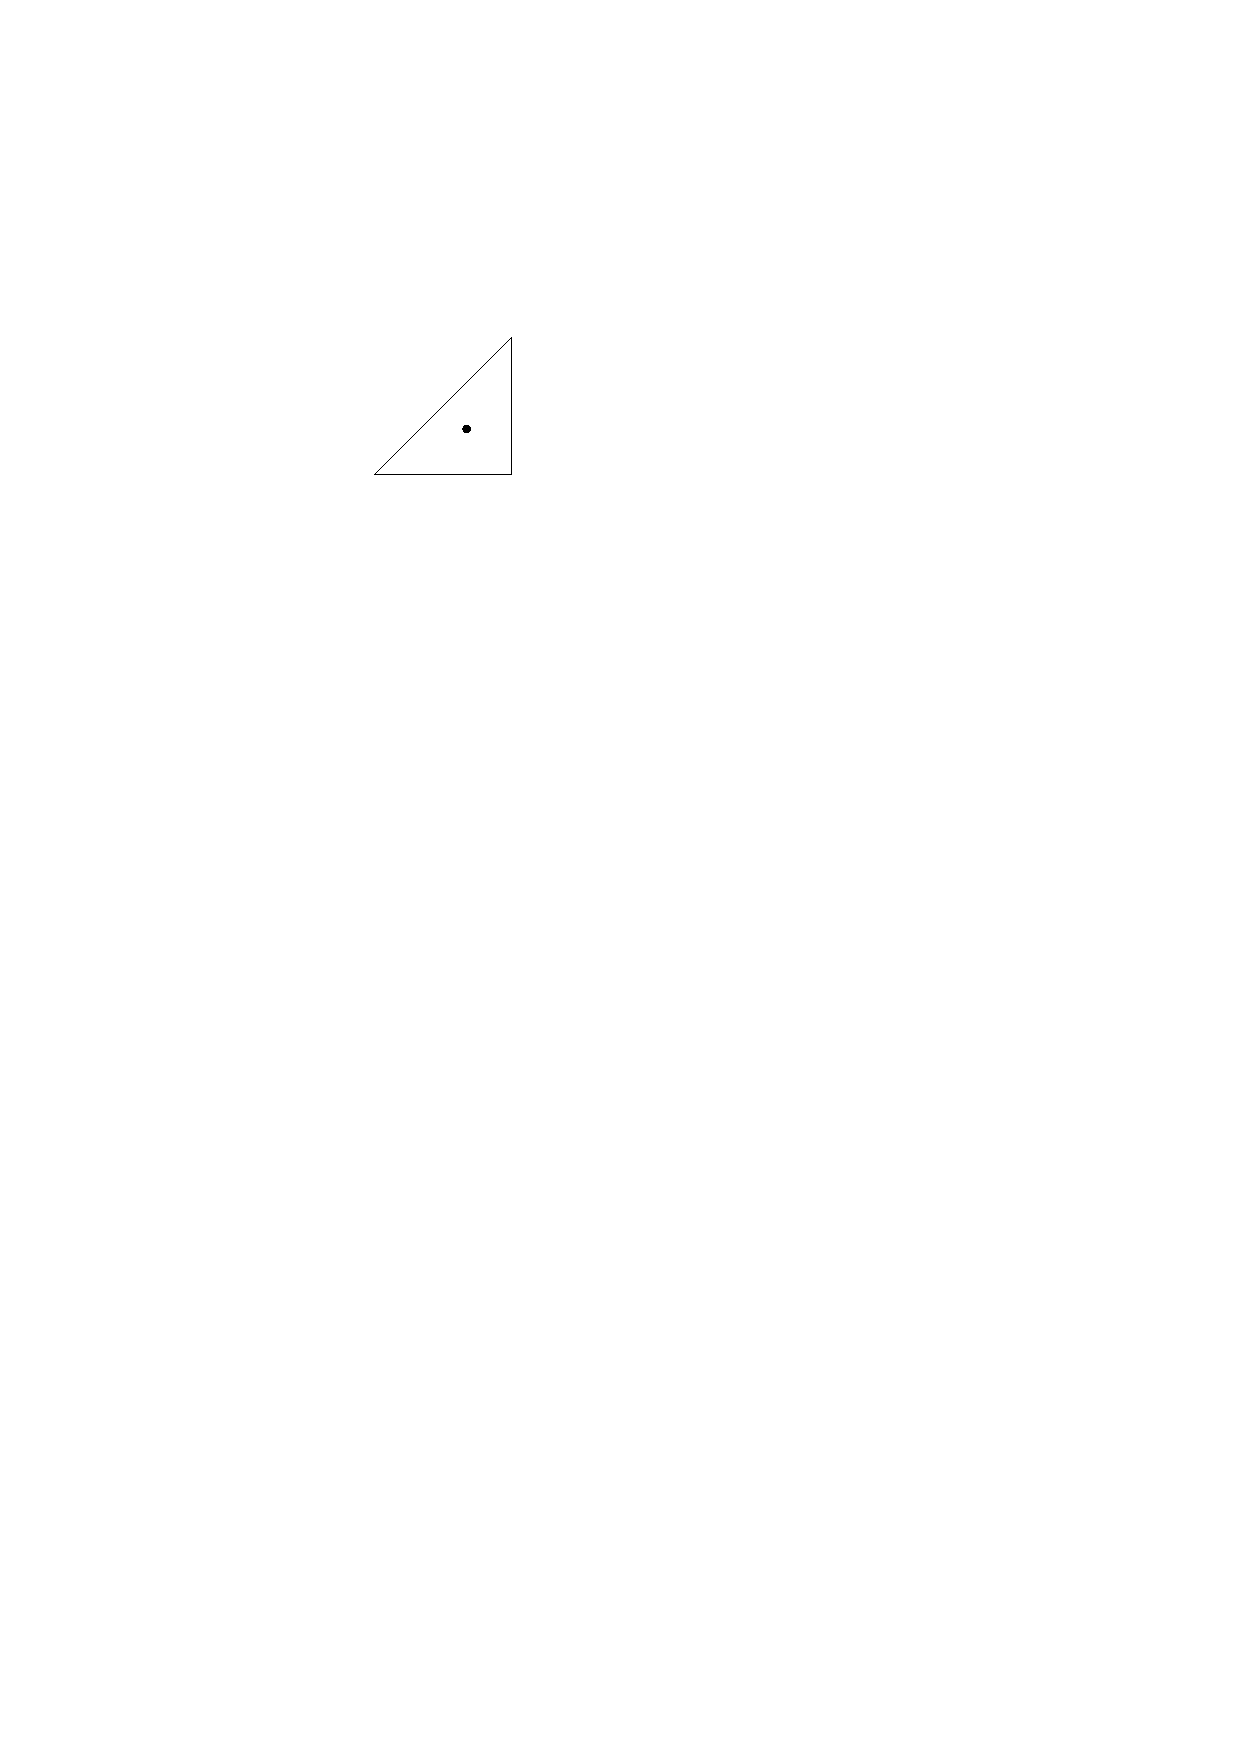
\includegraphics[scale=.8]{figs/killersb-7} \break%
           $\{\}$ \\
$\disjointc$ &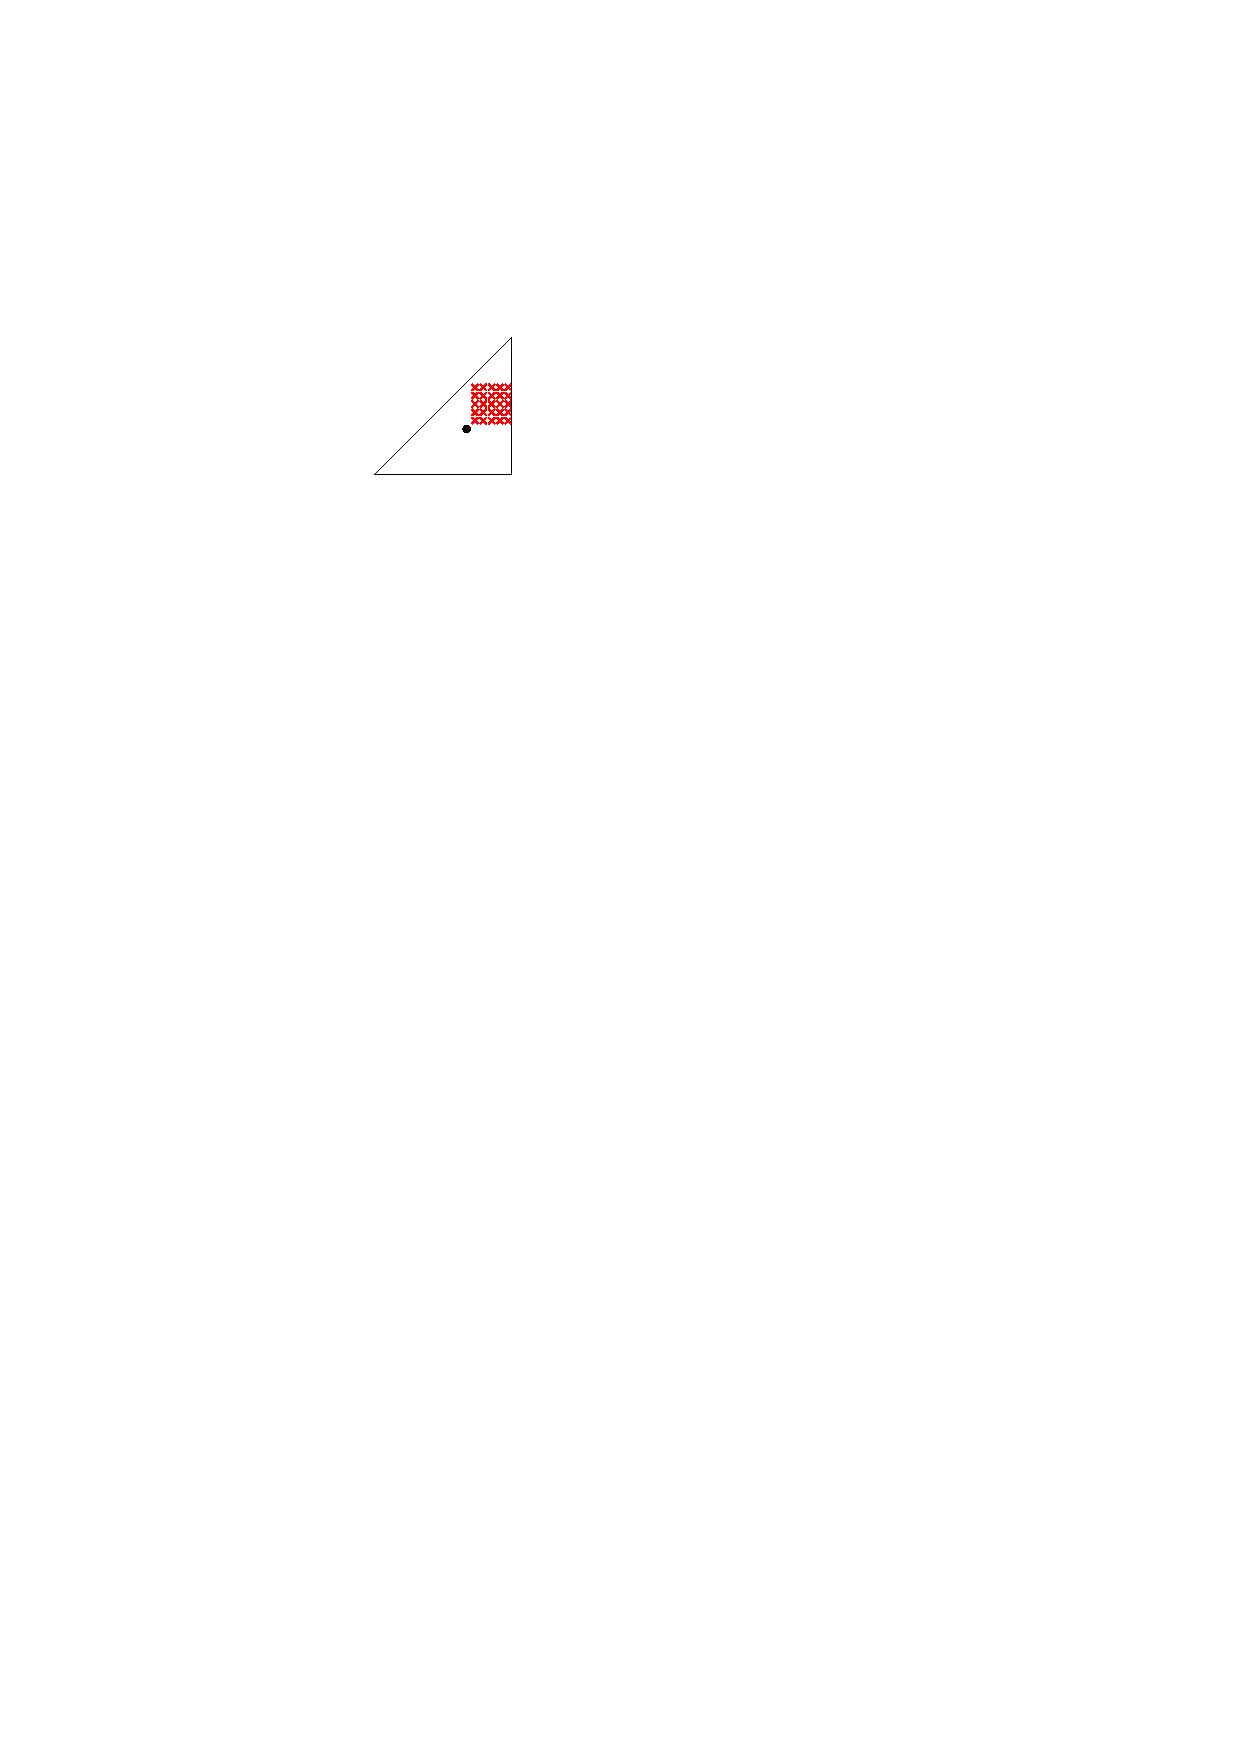
\includegraphics[scale=.8]{figs/killers-8} \break%
               $\{(x',y'): y < y' <x,\,\, x'>x\}$
         & 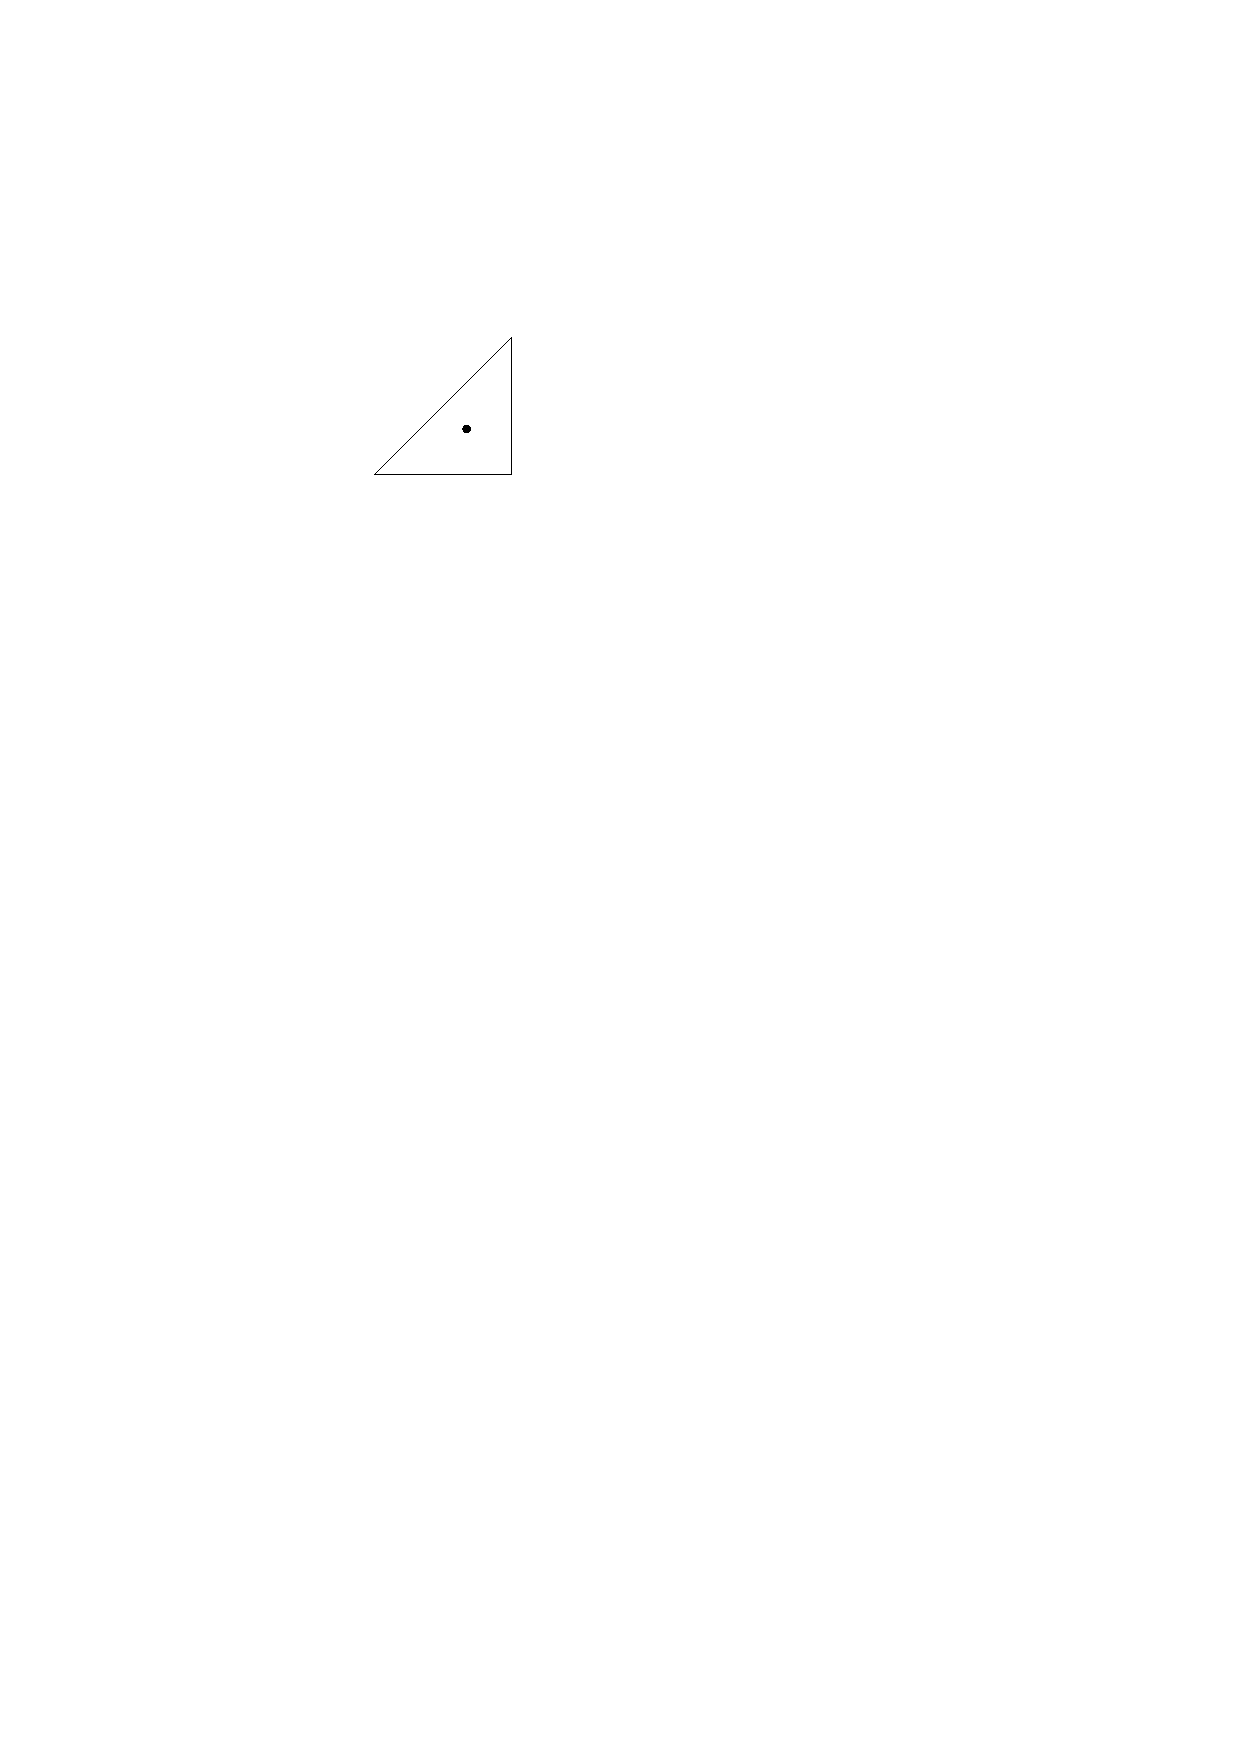
\includegraphics[scale=.8]{figs/killersb-8} \break%
           $\{\}$ \\
\end{tabular}
\end{center}
   \caption{The restrictions placed on the dot puzzle when for each of 
     the forbidden subconfigurations.}
   \tablabel{forbidden}
\end{table}



\begin{figure}
   \begin{center}
      \newlength{\ka}
      \setlength{\ka}{\textwidth}
      \addtolength{\ka}{-1cm}
      \begin{tabular}{c@{\hspace{1cm}}c}
        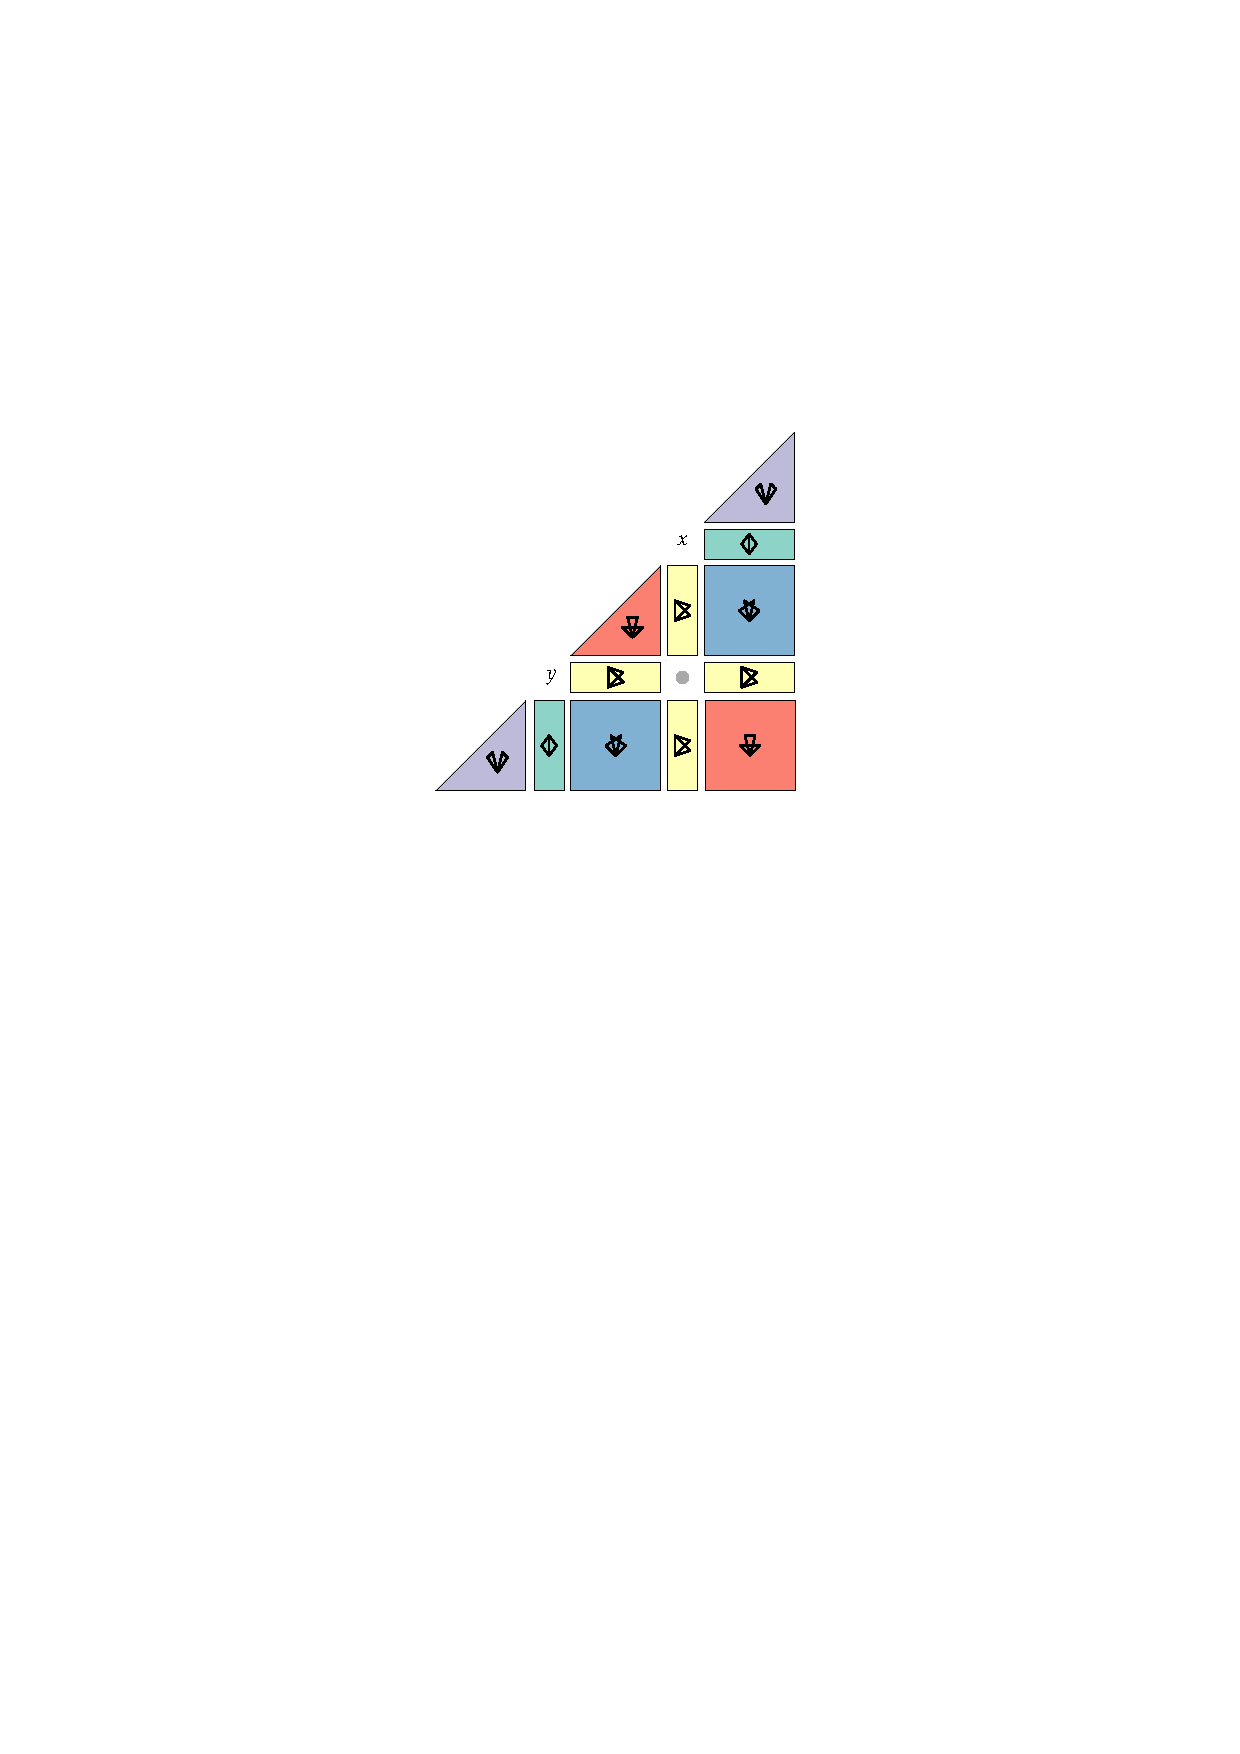
\includegraphics[width=.48\ka]{figs/crapper-2} & 
        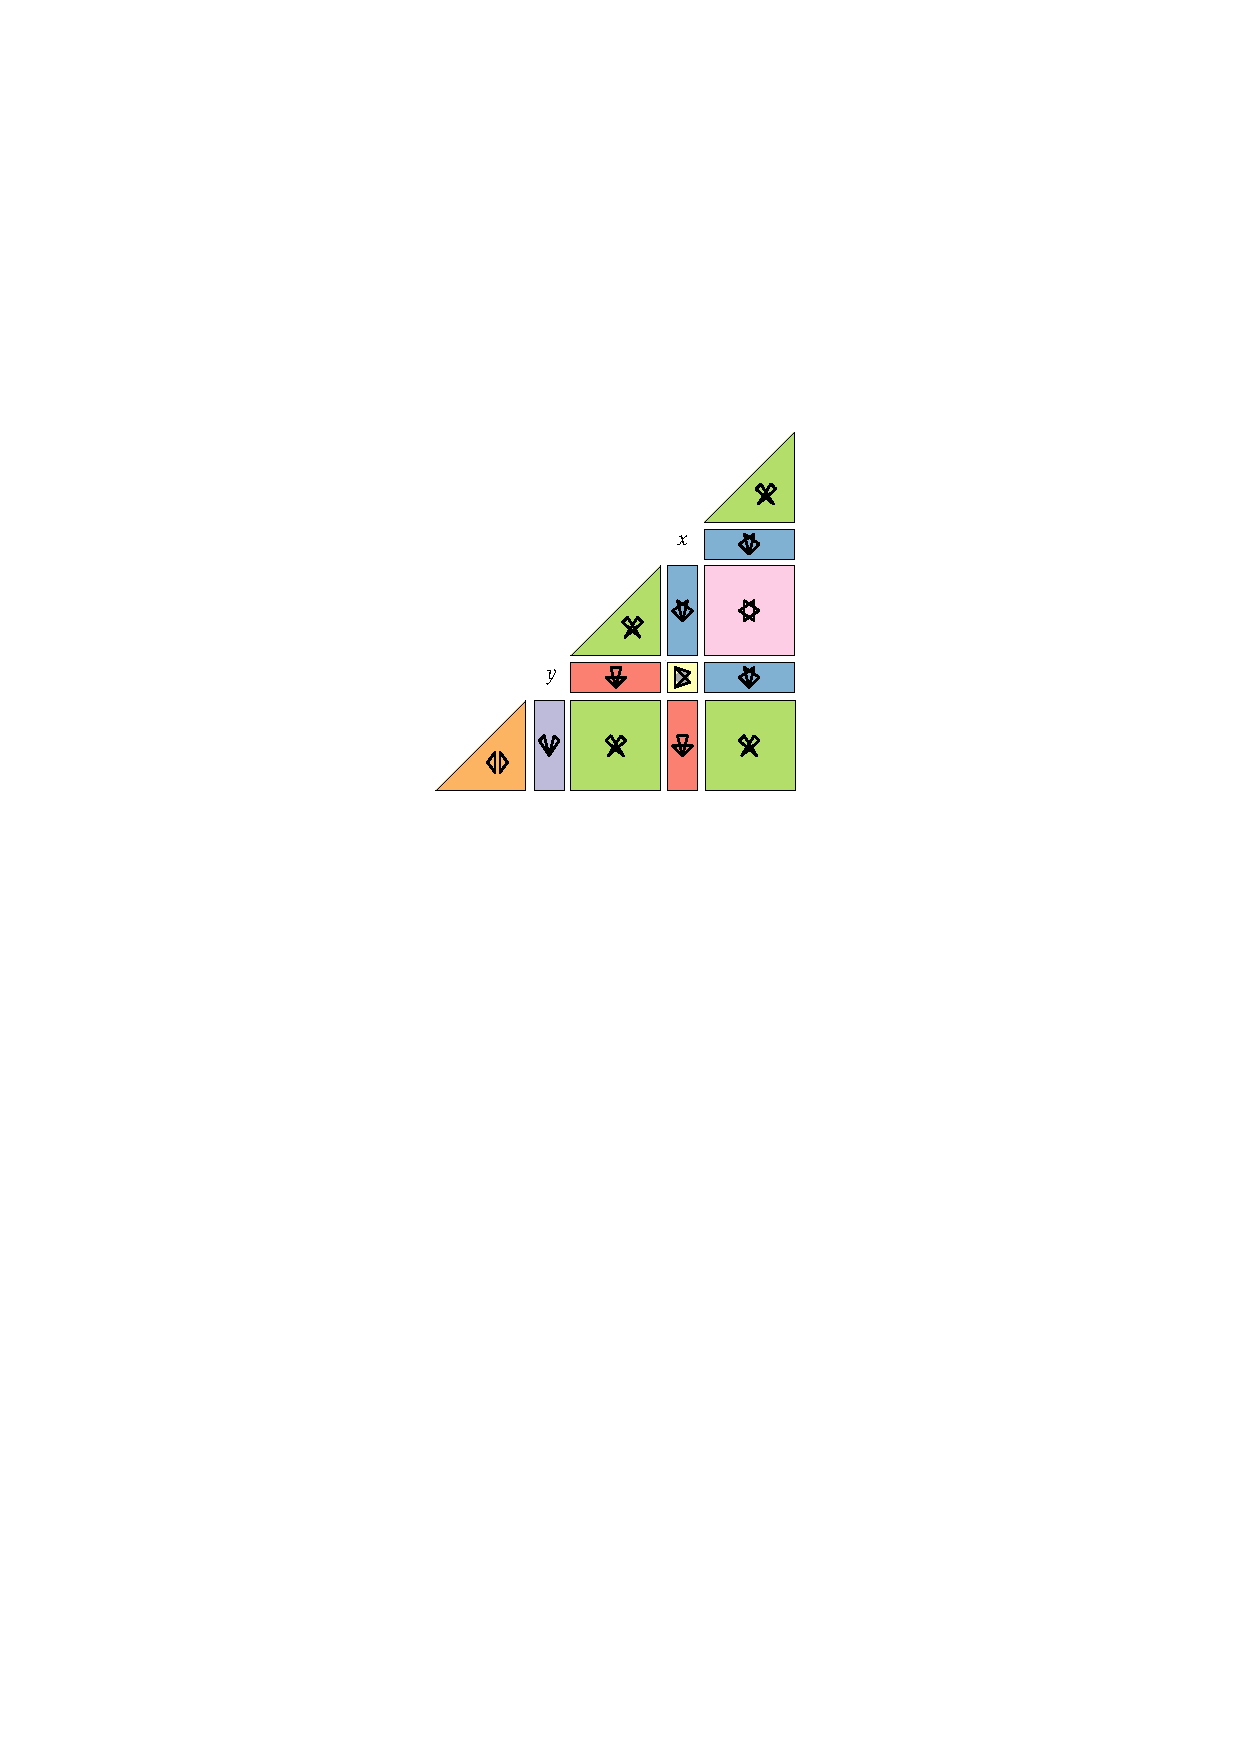
\includegraphics[width=.48\ka]{figs/crapper-1} \\
        (a) & (b)
      \end{tabular}
   \end{center}
   \caption{The regions killed by forbidden configurations during (a)~the current round and (b)~subsequent rounds.}
   \figlabel{forbidden-color}
\end{figure}
\section{Some Bounds}

We say that a point set is \emph{non-decreasing} (respectively,
increasing, non-increasing, decreasing) if, when sorted lexicographically,
the $y$ coordinates of the points form a non-decreasing (respectively,
increasing, non-increasing, decreasing) sequence.

From \tabref{forbidden}, some previous upper bounds naturally fall out.
For example, Bra\ss's results \cite{brass:turan} that $\ex(\vertexb)$
and $\ex(\vertexc)$ are each $O(n^2)$ come from the fact that the
points selected during a single round of the dot puzzle must be
non-decreasing (respectively, non-increasing); see the right column
of \tabref{forbidden}.  This immediately implies that one can select at
most $2n-2$ points during a single round of the dot puzzle game, for a
total of at most $2n^2-2n$ points during all $n$ rounds.  (Note, in the
top/bottom view, the bound on the number of the points selected during a
single round is a bound on the number of triangles incident to a bottom
vertex.)  The bounds $\ex(\vertexb)\in O(n^2)$ and $\ex(\vertexc)\in
O(n^2)$ then immediately follow from \lemref{top-bottom}.

Similarly, we can almost recover the result of Bra\ss, Rote and
Swanepoel \cite{brass.rote.ea:triangles} on $\ex(\disjointa, \disjointb,
\vertexa,\vertexb)$. 
By forbidding $\vertexb$, we have the rule
\begin{center}
  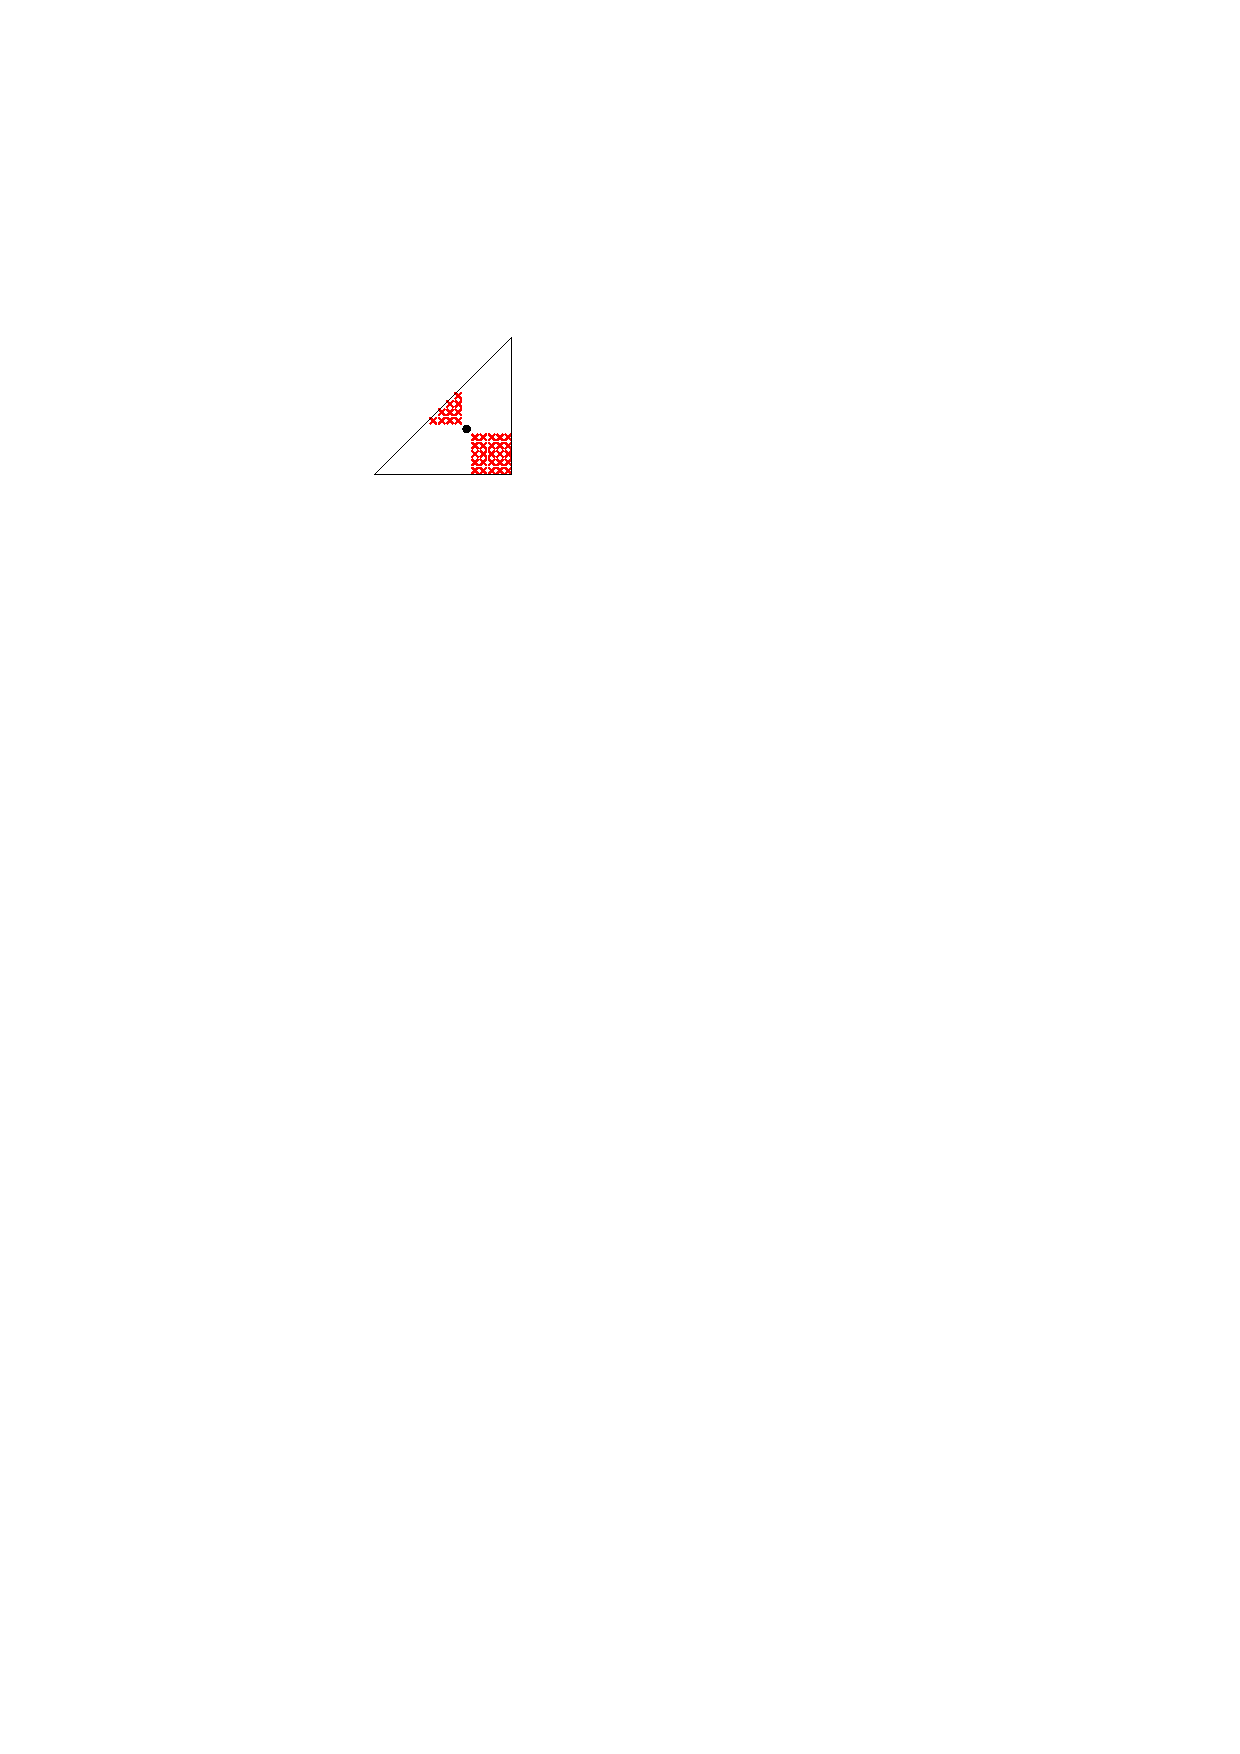
\includegraphics{figs/killersb-4} \enspace ,
\end{center}
which ensures that the set of points taken during a single round form an increasing point set.  From the forbidden configurations $\vertexa$,
$\vertexb$, $\disjointa$, and $\disjointb$, we obtain the rule
\begin{center}
  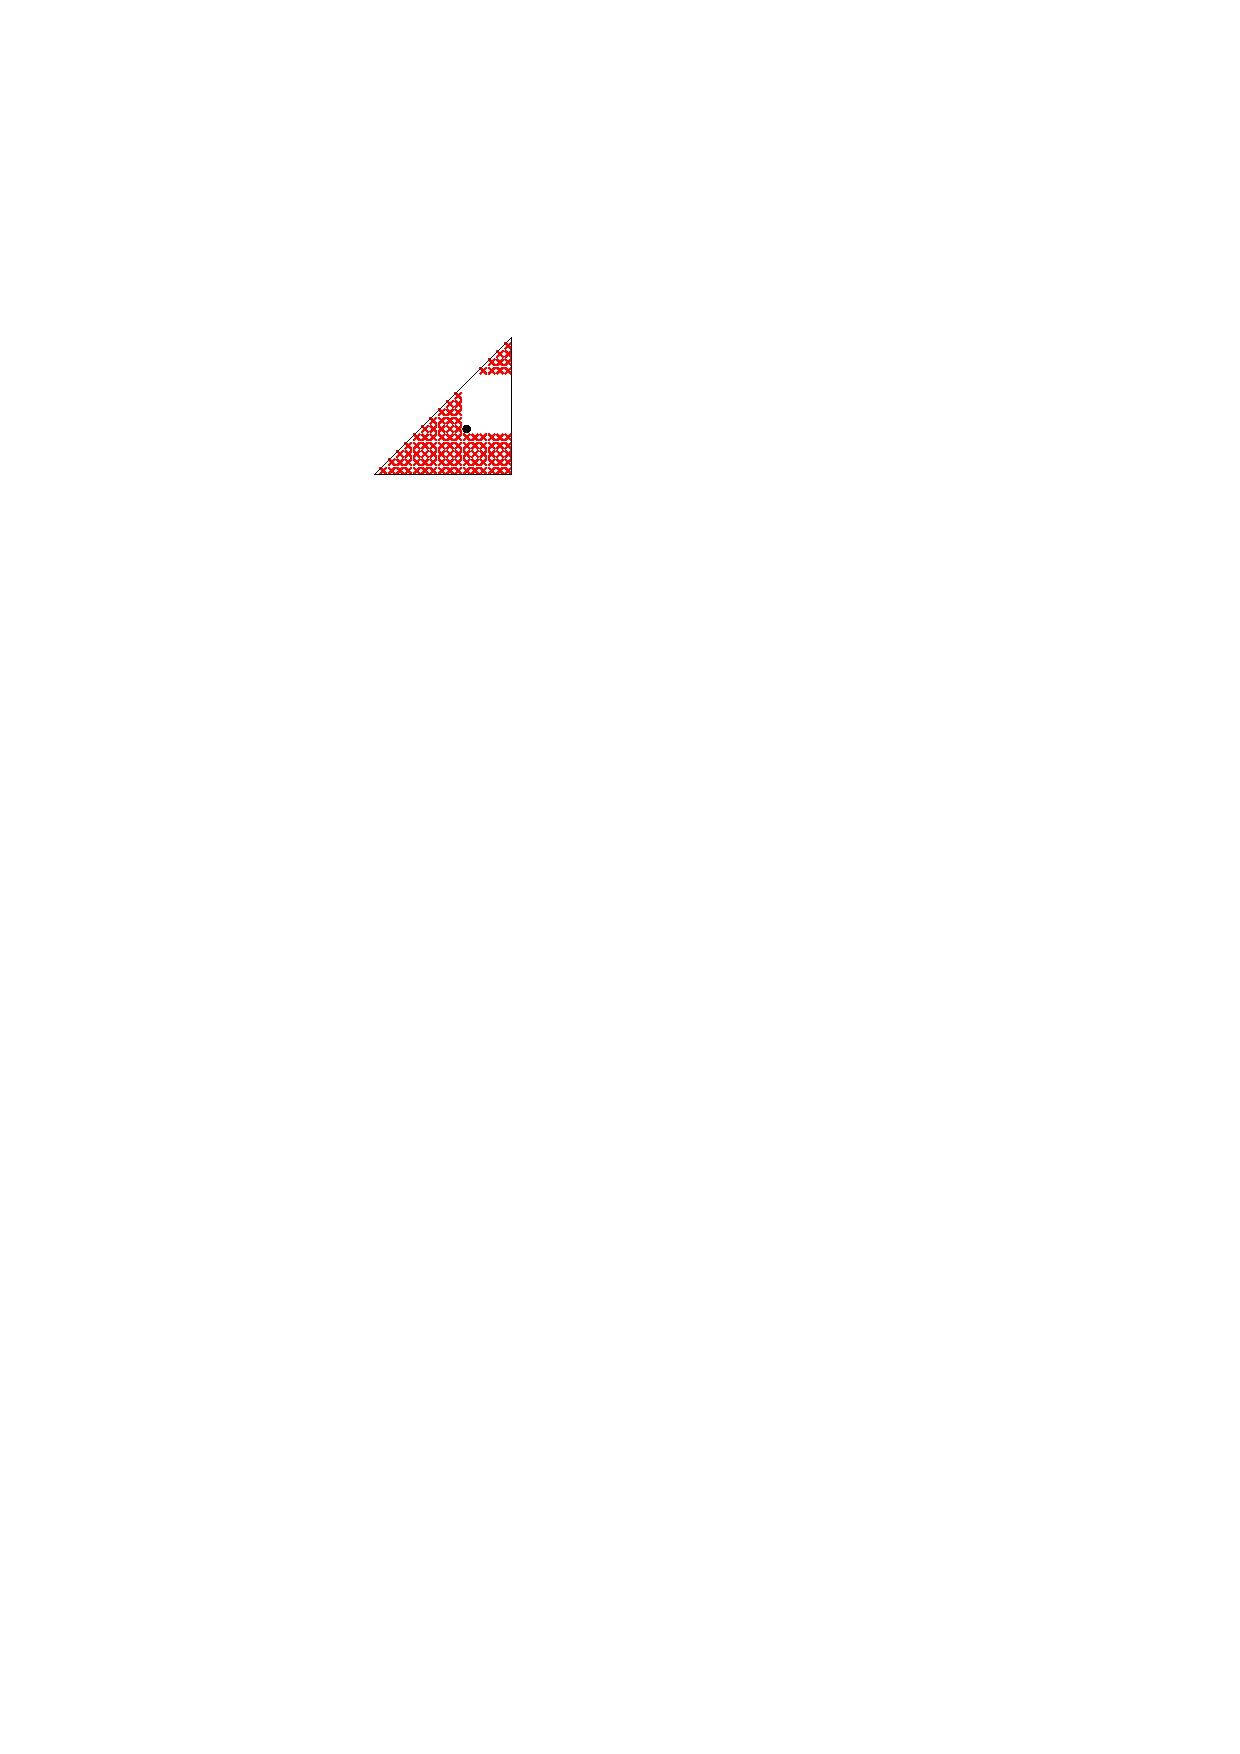
\includegraphics{figs/killers-9}
\end{center}
for which points are disallowed in subsequent rounds.  This rule ensures
that, after round $i$ any points chosen are either the topmost-rightmost
point in $Q_i$ or are above and to the right of this point.  Taken
together, these rules imply that
\[
    \sum_{i=1}^n|Q_i| \le 3n-2 \enspace ,
\]
Since the union of $Q_i$ is an increasing sequence (whose length is
therefore at most $2n-2$), and each $Q_i$ shares at most one point with
$Q_{i+1}$.  The bound $\ex(\disjointa, \disjointb, \vertexa,\vertexb)\in
O(n\log n)$ then follows from \lemref{top-bottom}.

For round $i$

Now, with our tools in hand, we are ready to study some problems.

\begin{thm}\thmlabel{blech}
  $\ex(n,\{\edgea,\vertexb,\vertexc\}) \in O(n\log n)$.
\end{thm}

\begin{proof}
  Since we forbid $\vertexb$, we know that the set of points taken
  during each round forms an increasing point set.  In particular,
  within a single round of the dot-puzzle we can take at most
  one point from each column.   Taking the union of the rules
  for $\edgea$, $\vertexb$, and $\vertexc$, we obtain the rule
  \begin{center}
     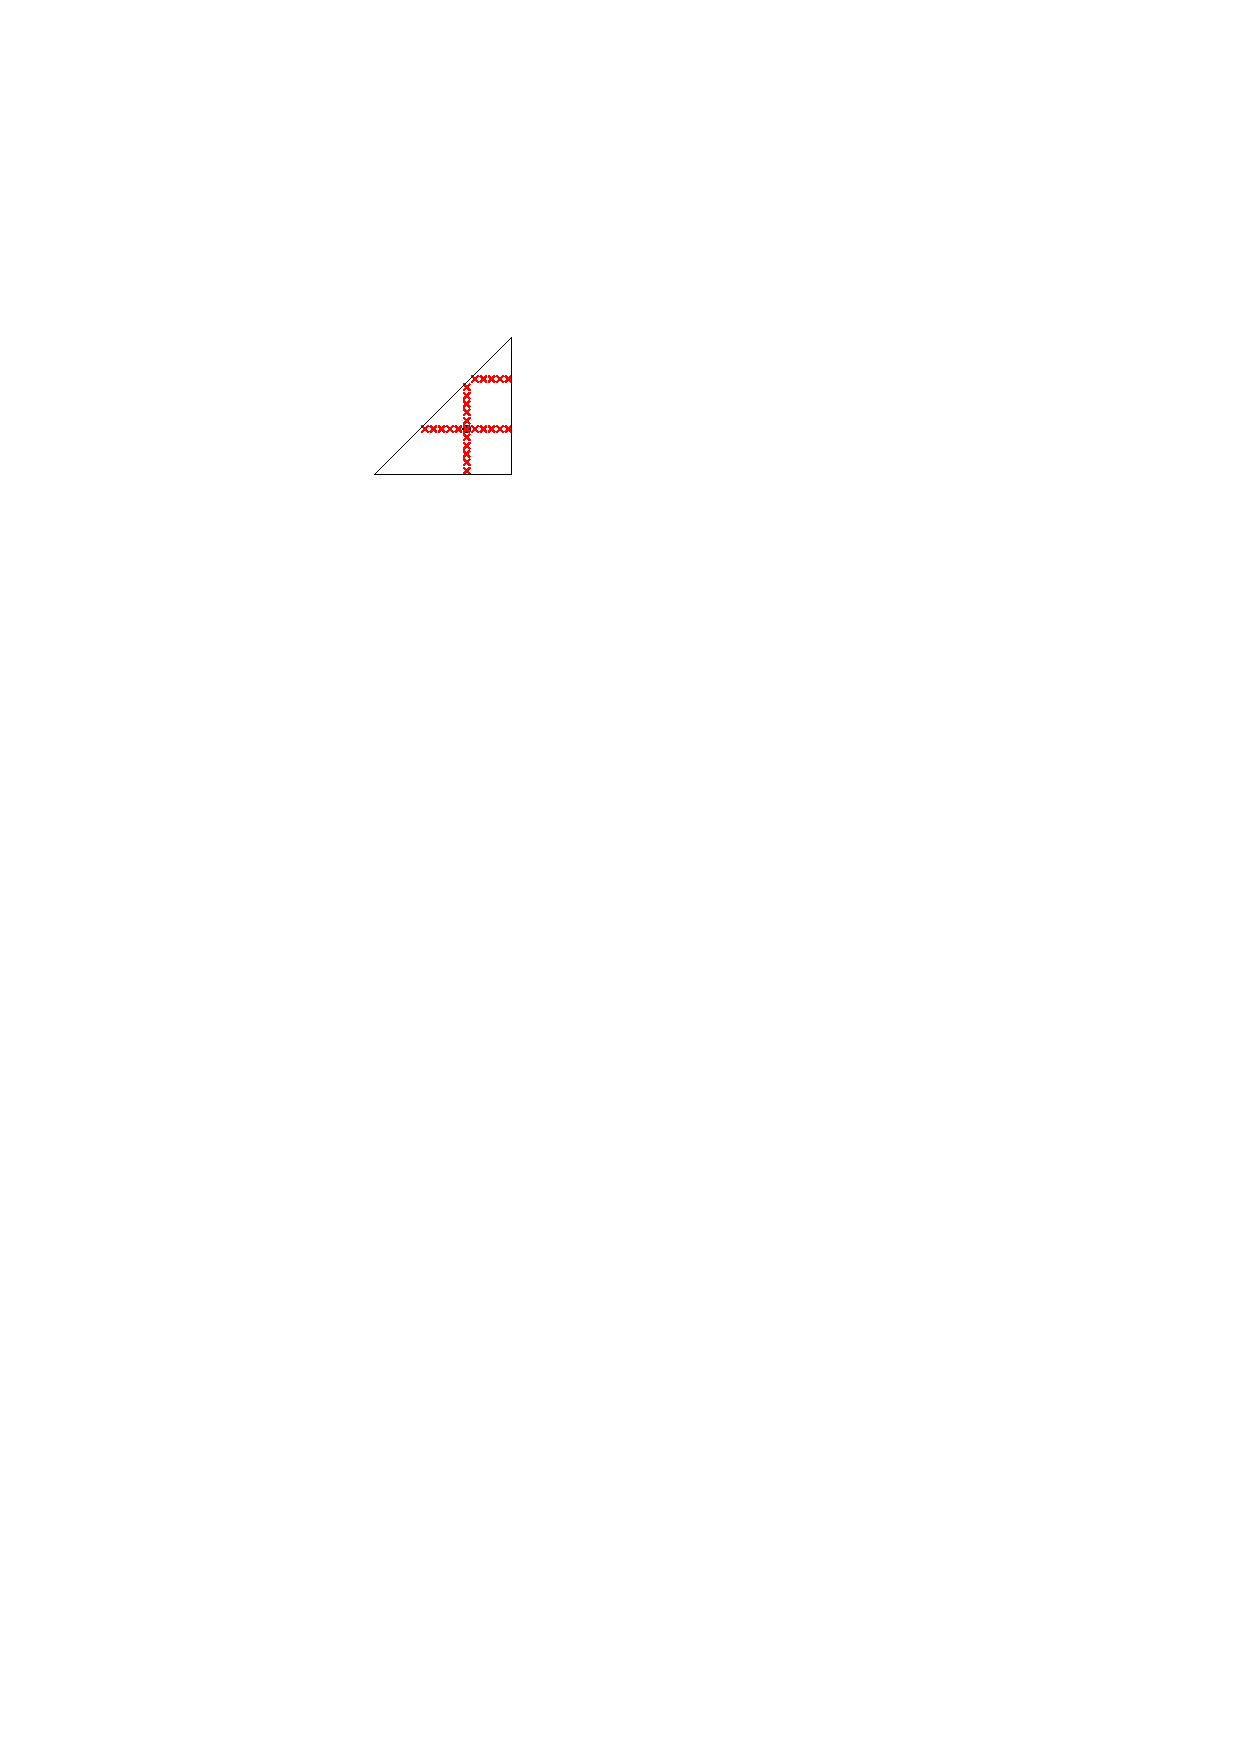
\includegraphics{figs/killers-10}
  \end{center}
  which ensures that during subsequent rounds we can not take a point from
  any column used in the previous round.  Thus, the sets $Q_1,\ldots,Q_n$
  contain at most one point from each column and have total size at
  most $n-1$.  This proves that, in the top-bottom view, we have at most
  $n-1$ triangles and the theorem then follows from \lemref{top-bottom}.
\end{proof}

I have the following two conjectures that are based on the fact that the
only large examples I know of for $\disjointb$ configurations repeatedly
use the same dots (and they all lie on a common vertical or horizontal
line).


\begin{lem}\lemlabel{survivor-structure}
  Let $S\subseteq Q$, $|S|\ge 1$. Then, $\survivors(\{\disjointb\},S)$
  is contained in of a triangular region $T=\{(x,y)\in Q: x<\ymin(S)\}$,
  a rectangular region $R\subseteq\{(x,y)\in Q: \xmax(S) \le x, ymax(S)\le
  y\le \xmax(S)\}$, and a set $L$ of $O(1)$ additional horizontal and vertical lines.
\end{lem}

\begin{thm}
  $\ex(n,\{\edgea,\disjointb\}) \in O(n\log n)$.
\end{thm}

\begin{proof}[Proof sketch]
  Without loss of generality, $|Q_1|\ge 1$.  Furthermore, forbidding
  $\edgea$ implies that $Q_1$ contains at most one point from each row
  and each column, so $|Q_i|\le n-1$.

  In round $i>1$, $\survivors(\{\edgea,\disjointb\},\bigcup_{j=1}^i
  Q_i)$ has the structure described in \lemref{survivor-structure}.
  Let $T_i$, $R_i$ and $L_i$ denote the sets $T$, $R$, and $L$ described
  in \lemref{survivor-structure} when applied to the point set
  $\survivors(\{\edgea,\disjointb\},\bigcup_{j=1}^i Q_i)$.

  Now, $Q_i$ contains at most one point in each row and each column, so it
  contains at most one point from each line in $L$ and $\ell_i\in O(1)$.
  Furthermore, if $T_{i}$ has a side length of $r$, then $T_{i+1}$ has a 
  side-length of at most $r-\min\{t_i-1,0\}$.



  Furthermore, if



  $Q_i$ contains $t$ points in $T$, then $\xmin(\bigcup_{j=1}^i Q_j) \le
  \xmin(\bigcup_{j=1}^{i-1}Q_j)-t$ (so $T$ loses at least $t$ columns).
  Similarly, if $Q_i$ contains $r$ points in $T$, then $R$ loses at
  least $r$ columns.
  
  Using the obvious notation, we have that
  \[
      \sum_{j=1}^n 
  \]


\end{proof}

\begin{thm}
  $\ex(\vertexb,\disjointb) \in O(n\log n)$.
\end{thm}

\begin{proof}[Proof sketch]
  Follows from \lemref{constant-degree} and the fact that the $\edgea$
  configuration prevents killinng selecting the same point twice.
\end{proof}

\begin{thm}
    $\ex(\vertexc,\disjointb) \in O(n\log n)$.
\end{thm}


\begin{conj}
    $\ex(\edgea,\vertexb) \in \Theta(n^{3/2})$.
\end{conj}




\bibliographystyle{plain}
\bibliography{turan}

\end{document}


